% =============================================================
%  FPGA与VHDL考试复习全书
%  围绕23个重点电路构建的完整知识体系
% =============================================================

\documentclass[12pt,a4paper,openany]{ctexbook}

% =============================================================
%  中文支持与字体
% =============================================================
\usepackage{fontspec}
\setmainfont{Times New Roman}
\setCJKmainfont{SimSun}[AutoFakeBold=2.5]
\setCJKsansfont{SimHei}
\setCJKmonofont{SimSun}

% =============================================================
%  页面布局
% =============================================================
\usepackage[top=2.5cm,bottom=2.5cm,left=2.8cm,right=2.5cm]{geometry}
\usepackage{fancyhdr}
\pagestyle{fancy}
\fancyhf{}
\fancyhead[LE,RO]{\thepage}
\fancyhead[LO]{\nouppercase{\leftmark}}
\fancyhead[RE]{\nouppercase{\rightmark}}
\renewcommand{\headrulewidth}{0.4pt}

% =============================================================
%  数学与公式
% =============================================================
\usepackage{amsmath,amssymb,amsfonts}
\usepackage{mathtools}

% =============================================================
%  图形与电路图
% =============================================================
\usepackage{tikz}
\usepackage{circuitikz}
\usepackage{tikz-timing}
\usetikzlibrary{arrows,shapes,chains,matrix,positioning,scopes,calc,
                decorations.pathreplacing,decorations.markings,fit,
                backgrounds,patterns,automata}

% =============================================================
%  表格
% =============================================================
\usepackage{tabularx}
\usepackage{booktabs}
\usepackage{multirow}
\usepackage{makecell}
\usepackage{longtable}
\usepackage{colortbl}

% =============================================================
%  代码清单 (VHDL)
% =============================================================
\usepackage{listings}
\usepackage{xcolor}

\definecolor{vhdlcomment}{rgb}{0.0,0.5,0.0}
\definecolor{vhdlkeyword}{rgb}{0.0,0.0,0.8}
\definecolor{vhdlstring}{rgb}{0.6,0.1,0.1}
\definecolor{vhdlnumber}{rgb}{0.5,0.5,0.5}
\definecolor{vhdlbackground}{rgb}{0.97,0.97,0.97}

\lstdefinelanguage{VHDL}{
  morekeywords={
    library,use,all,entity,is,port,in,out,inout,end,
    architecture,of,begin,process,signal,variable,constant,
    type,subtype,array,range,to,downto,others,then,
    elsif,else,case,when,for,loop,generate,not,and,
    or,xor,nand,nor,xnor,mod,rem,abs,component,generic,
    map,wait,on,until,after,report,severity,assert,
    std_logic,std_logic_vector,bit,bit_vector,integer,
    boolean,character,string,positive,natural,unsigned,signed,
    ieee,std_logic_1164,std_logic_arith,std_logic_unsigned,
    numeric_std,rising_edge,falling_edge,event,clk,rst,reset
  },
  % Note: 'if' is a TeX primitive - handle it via emph to avoid conflicts
  emph={if},
  emphstyle=\color{vhdlkeyword}\bfseries,
  sensitive=true,
  morecomment=[l]{--},
  morestring=[b]",
  morestring=[b]'
}[keywords,comments,strings]

\lstset{
  language=VHDL,
  basicstyle=\ttfamily\footnotesize,
  keywordstyle=\color{vhdlkeyword}\bfseries,
  commentstyle=\color{vhdlcomment}\itshape,
  stringstyle=\color{vhdlstring},
  numbers=left,
  numberstyle=\tiny\color{vhdlnumber},
  backgroundcolor=\color{vhdlbackground},
  frame=single,
  framerule=0.5pt,
  rulecolor=\color{gray!40},
  tabsize=2,
  breaklines=true,
  breakatwhitespace=false,
  captionpos=b,
  showstringspaces=false,
  xleftmargin=2em,
  xrightmargin=1em,
  aboveskip=1em,
  belowskip=1em
}

% =============================================================
%  超链接与书签
% =============================================================
\usepackage[colorlinks=true,
            linkcolor=blue!60!black,
            citecolor=green!50!black,
            urlcolor=blue!60!black]{hyperref}

% =============================================================
%  其他工具
% =============================================================
\usepackage{enumitem}
\usepackage{caption}
\usepackage{subcaption}
\usepackage{float}
\usepackage{placeins}
\usepackage{environ}
\usepackage{framed,color}

% =============================================================
%  自定义命令
% =============================================================

% 重点知识框
\NewEnviron{keypoint}[1][重点]{%
  \begin{center}
  \begin{tikzpicture}
  \node[draw=blue!60,fill=blue!5,rounded corners=5pt,
        inner sep=8pt,text width=0.9\textwidth,align=left]
  {\textbf{#1：}\BODY};
  \end{tikzpicture}
  \end{center}}

% 考试技巧框
\NewEnviron{examtip}[1][考试技巧]{%
  \begin{center}
  \begin{tikzpicture}
  \node[draw=red!60,fill=red!3,rounded corners=5pt,
        inner sep=8pt,text width=0.9\textwidth,align=left]
  {\textbf{\textcolor{red!70!black}{#1：}}\BODY};
  \end{tikzpicture}
  \end{center}}

% 设计流程框
\NewEnviron{designflow}[1][设计流程]{%
  \begin{center}
  \begin{tikzpicture}
  \node[draw=teal!60,fill=teal!3,rounded corners=5pt,
        inner sep=8pt,text width=0.9\textwidth,align=left]
  {\textbf{\textcolor{teal!70!black}{#1：}}\BODY};
  \end{tikzpicture}
  \end{center}}

% 逐拍分析
\NewEnviron{beatanalysis}[1][逐拍分析]{%
  \begin{center}
  \begin{tikzpicture}
  \node[draw=orange!80,fill=orange!3,rounded corners=5pt,
        inner sep=8pt,text width=0.9\textwidth,align=left]
  {\textbf{\textcolor{orange!80!black}{#1：}}\BODY};
  \end{tikzpicture}
  \end{center}}

% 变式详解框
\newenvironment{detailbox}[1][详解]
  {\begin{oframed}\textbf{\large #1}\\[3pt]}
  {\end{oframed}}

% 考试聚焦框
\newenvironment{examfocus}[1][考试聚焦]
  {\begin{oframed}\textbf{\textcolor{red!70!black}{#1}}\\[3pt]}
  {\end{oframed}}

% 真值表命令
\newcommand{\ttable}[1]{%
  \begin{center}
  \begin{tabular}{#1}
}

\newcommand{\ettable}{%
  \end{tabular}
  \end{center}
}

% 状态标记
\newcommand{\state}[1]{$\langle #1 \rangle$}

% D触发器符号
\newcommand{\DFF}{D触发器}

% 上升沿
\newcommand{\rising}{$\uparrow$}

% 重点
\newcommand{\imp}[1]{\textbf{\textcolor{red}{#1}}}

% 时钟拍
\newcommand{\clktick}[1]{\textbf{时钟第#1拍}}

% =============================================================
%  文档信息
% =============================================================
\title{\Huge \textbf{数字电路与VHDL设计教程}\\[0.5cm]
       \Large 围绕23个重点电路构建的完整知识体系}
\author{myp}
\date{\today}

\begin{document}

\maketitle

\tableofcontents

% =============================================================
%  前言
% =============================================================
\chapter*{前言}
\addcontentsline{toc}{chapter}{前言}

\section*{本书的目标}

这本书不是一本传统的数字电路教材。

传统教材的写法是：数制→逻辑门→布尔代数→卡诺图→组合逻辑→时序逻辑→... \par

这本书的写法是：\par
\begin{center}
\fbox{%
\begin{minipage}{0.85\textwidth}
\textbf{以电路为主线，反向展开其所涉及的数字电路知识。}

电路 → 原理 → 状态变化 → 设计思想 → 设计模板 → VHDL实现 → 考试变式
\end{minipage}%
}
\end{center}

\section*{本书的结构}

本书分为十个部分：

\begin{description}
  \item[第一部分] 组合逻辑电路体系 —— 编码器、译码器、MUX、比较器、加法器
  \item[第二部分] D触发器体系 —— 从"为什么需要存储"开始，建立状态与记忆的概念
  \item[第三部分] 计数器体系 —— 用统一框架串起所有模值计数器
  \item[第四部分] 分频器体系 —— 从状态变化解释频率减半的物理过程
  \item[第五部分] 序列发生器体系 —— 多种实现方案比较
  \item[第六部分] 移位寄存器体系 —— 数据流动的逐拍分析
  \item[第七部分] 环形计数器体系 —— 从移位寄存器推导环形计数器
  \item[第八部分] 序列检测器体系 —— 状态机的核心应用
  \item[第九部分] VHDL专题 —— 每种VHDL写法综合成什么硬件
  \item[第十部分] 考试训练体系 —— 每类电路20+道变式题
\end{description}

\section*{如何使用本书}

\begin{enumerate}
  \item \textbf{如果你时间充裕}：从头到尾，按顺序阅读。
  \item \textbf{如果你时间紧张}：直接跳到对应电路的章节，每章是自包含的。
  \item \textbf{如果你只需要刷题}：直接看第十部分。
\end{enumerate}

\section*{关于"为什么"}

本书最重要的一个原则是：

\begin{center}
\fbox{%
\begin{minipage}{0.85\textwidth}
\large \textbf{不讲"是什么"，只讲"为什么"。}

每一个设计决策都有原因。

每一个公式都有推导过程。

每一个状态变化都有逐拍分析。
\end{minipage}%
}
\end{center}

\section*{关于代码}

\textbf{不要在理解电路之前看代码。}

如果你看到一个电路，第一反应是"它的VHDL怎么写"，那你就学反了。

正确的顺序是：

\begin{enumerate}
  \item 理解这个电路要解决什么问题
  \item 理解它的输入输出关系
  \item 理解它的内部工作原理
  \item 理解为什么这样设计
  \item 然后，VHDL只是这些理解的翻译
\end{enumerate}

如果你理解了设计逻辑，任何VHDL变式你都能自己写出来。

\section*{写在前面}

这套书可能和你在学校里见过的任何一本数字电路教材都不一样。

它不讲数制，不讲卡诺图，不从逻辑代数开始。(它默认你已经学过这些了，并且已经能够利用这些工具分析电路了。)

它从数字电路中典型的23个电路开始。

每一个电路，我们不讲废话，只讲三件事：

\begin{enumerate}
  \item \textbf{它为什么存在}（解决了什么问题）
  \item \textbf{它是怎么工作的}（原理和状态变化）
  \item \textbf{怎么用它解题}（考试变式和解题模板）
\end{enumerate}

祝学习顺利。

\vspace{2cm}
\hfill ———myp


% =============================================================
%  第一部分：组合逻辑电路体系
% =============================================================
\part{组合逻辑电路体系}

\chapter{8-3编码器}

\section{第一步：解决什么问题}

想象一个场景：你的FPGA有8个按键，编号0到7。用户按下其中一个按键。

\begin{itemize}
  \item 如果用8根信号线传给处理器，需要8个引脚——浪费资源
  \item 更好的方案：用3根信号线传递"哪个按键被按下"的信息
  \item 因为 $2^3 = 8$，3根线恰好能表示8种状态
\end{itemize}

\textbf{编码器（Encoder）的本质}：将 $2^n$ 个输入信号，压缩成 $n$ 位二进制输出。

\begin{keypoint}[编码器的本质]
编码器 = 信号压缩器：$2^n$ 个输入 $\to$ $n$ 位输出

8-3编码器：8个输入 $\to$ 3位输出
\end{keypoint}

\section{第二步：输入输出关系}

\begin{itemize}
  \item \textbf{输入}：$I_0, I_1, I_2, I_3, I_4, I_5, I_6, I_7$（8个输入信号，高电平有效）
  \item \textbf{输出}：$Y_2, Y_1, Y_0$（3位二进制编码输出）
  \item \textbf{约束}：任意时刻最多只有一个输入为1
\end{itemize}

当 $I_k = 1$（且其他输入为0）时，输出 $(Y_2 Y_1 Y_0)$ 应该等于 $k$ 的二进制表示。

\section{第三步：真值表}

\begin{center}
\begin{tabular}{|c|c|c|c|}
\hline
\textbf{有效输入} & $Y_2$ & $Y_1$ & $Y_0$ \\
\hline
$I_0 = 1$ & 0 & 0 & 0 \\
$I_1 = 1$ & 0 & 0 & 1 \\
$I_2 = 1$ & 0 & 1 & 0 \\
$I_3 = 1$ & 0 & 1 & 1 \\
$I_4 = 1$ & 1 & 0 & 0 \\
$I_5 = 1$ & 1 & 0 & 1 \\
$I_6 = 1$ & 1 & 1 & 0 \\
$I_7 = 1$ & 1 & 1 & 1 \\
\hline
\end{tabular}
\end{center}

\section{第四步：逻辑推导}

观察真值表，找出每个输出位什么时候为1：

\begin{itemize}
  \item $Y_2 = 1$ 当 $I_4=1$ 或 $I_5=1$ 或 $I_6=1$ 或 $I_7=1$
  \item $Y_1 = 1$ 当 $I_2=1$ 或 $I_3=1$ 或 $I_6=1$ 或 $I_7=1$
  \item $Y_0 = 1$ 当 $I_1=1$ 或 $I_3=1$ 或 $I_5=1$ 或 $I_7=1$
\end{itemize}

因此，逻辑表达式为：

\begin{align}
  Y_2 &= I_4 + I_5 + I_6 + I_7 \\
  Y_1 &= I_2 + I_3 + I_6 + I_7 \\
  Y_0 &= I_1 + I_3 + I_5 + I_7
\end{align}

每个输出位都是若干输入的\textbf{逻辑或（OR）}。

\section{第五步：结构化设计}

8-3编码器内部结构：

\begin{center}
\begin{tikzpicture}
  % Inputs
  \foreach \x in {0,...,7} {
    \node (I\x) at (0, -1.2*\x) {$I_\x$};
  }
  % OR gates
  \node[american or port,rotate=-90] (or2) at (4,-2.5) {};
  \node[american or port,rotate=-90] (or1) at (4,-5) {};
  \node[american or port,rotate=-90] (or0) at (4,-7.5) {};

  % Outputs
  \node (Y2) at (5.5,-2.5) {$Y_2$};
  \node (Y1) at (5.5,-5) {$Y_1$};
  \node (Y0) at (5.5,-7.5) {$Y_0$};

  % Connections for Y2
  \draw (I4) -- ++(1.5,0) |- (or2.in 1);
  \draw (I5) -- ++(1.5,0) |- (or2.in 2);
  \draw (I6) -- ++(2.0,0) |- (or2.in 1);
  \draw (I7) -- ++(2.5,0) |- (or2.in 2);

  \draw (or2.out) -- (Y2);
\end{tikzpicture}
\end{center}

\textbf{设计规律}：$Y_k$ 的输出 = 所有编号第 $k$ 位为1的输入的OR。

\begin{itemize}
  \item $Y_2$（bit 2 = 4的位）：连接 $I_4, I_5, I_6, I_7$（这些编号的二进制第2位都是1）
  \item $Y_1$（bit 1 = 2的位）：连接 $I_2, I_3, I_6, I_7$
  \item $Y_0$（bit 0 = 1的位）：连接 $I_1, I_3, I_5, I_7$
\end{itemize}

\section{第六步：为什么这样设计}

\begin{enumerate}
  \item \textbf{为什么用OR门？}

  观察真值表：对于 $Y_k$，任何使 $Y_k=1$ 的输入条件之间是"或"的关系——只要其中任何一个条件满足，$Y_k$ 就是1。

  \item \textbf{为什么输入之间存在约束？}

  如果两个输入同时为1，OR门的输出仍然是1，但编码结果就错了（对应了另一个不需要的编码）。所以编码器假设同一时刻只有一个输入有效。

  \item \textbf{优先级编码器的改进动机？}

  当多个输入同时有效时，普通编码器产生错误输出。优先级编码器增加了优先级逻辑——一般编号大的输入优先级高。这需要用if-else级联逻辑而非简单OR门。
\end{enumerate}

\section{第七步：考试常见变式}

\begin{enumerate}
  \item \textbf{变式1：16-4编码器}

  将16个输入编码为4位输出。原理完全相同，只是规模扩大。$Y_3 = I_8 + I_9 + \cdots + I_{15}$，以此类推。

  \item \textbf{变式2：优先级编码器（Priority Encoder）}

  允许同时多个输入为1，输出最高优先级输入的编号。这是考试的热门考点。

  优先级编码器的真值表（优先级：$I_7 > I_6 > \cdots > I_0$）：

  \begin{center}
  \begin{tabular}{|c|c|c|c|c|}
  \hline
  $I_7$ & $I_6$ & $I_5$ & ... & $(Y_2 Y_1 Y_0)$ \\
  \hline
  1 & x & x & ... & 111 \\
  0 & 1 & x & ... & 110 \\
  0 & 0 & 1 & ... & 101 \\
  \vdots & \vdots & \vdots & \ddots & \vdots \\
  \hline
  \end{tabular}
  \end{center}

  \item \textbf{变式3：带使能端的编码器}

  增加一个Enable输入，E=1时编码器正常工作，E=0时所有输出为0。

  \item \textbf{变式4：输出有效的编码器}

  增加一个GS（Group Select）输出，当任何输入有效时GS=1，否则GS=0。用于区分"选择了$I_0$"（输出000）和"没有选择"（输出也是000）。

  \item \textbf{变式5：低电平有效的编码器}

  输入和输出都是低电平有效（即0表示有效，1表示无效）。逻辑门类型可能需要相应改变。
\end{enumerate}

\section{第八步：VHDL实现}

\subsection{普通8-3编码器}

\begin{lstlisting}[caption={8-3编码器VHDL实现（if-else版本）}]
library ieee;
use ieee.std_logic_1164.all;

entity encoder_8to3 is
  port (
    I : in  std_logic_vector(7 downto 0);
    Y : out std_logic_vector(2 downto 0)
  );
end encoder_8to3;

architecture behavioral of encoder_8to3 is
begin
  process(I)
  begin
    case I is
      when "00000001" => Y <= "000";
      when "00000010" => Y <= "001";
      when "00000100" => Y <= "010";
      when "00001000" => Y <= "011";
      when "00010000" => Y <= "100";
      when "00100000" => Y <= "101";
      when "01000000" => Y <= "110";
      when "10000000" => Y <= "111";
      when others      => Y <= "000";
    end case;
  end process;
end behavioral;
\end{lstlisting}

\subsection{优先级编码器}

\begin{lstlisting}[caption={8-3优先级编码器（使用if-else级联）}]
library ieee;
use ieee.std_logic_1164.all;

entity priority_encoder_8to3 is
  port (
    I : in  std_logic_vector(7 downto 0);
    Y : out std_logic_vector(2 downto 0);
    GS: out std_logic
  );
end priority_encoder_8to3;

architecture behavioral of priority_encoder_8to3 is
begin
  process(I)
  begin
    GS <= '1';
    if    I(7) = '1' then Y <= "111";
    elsif I(6) = '1' then Y <= "110";
    elsif I(5) = '1' then Y <= "101";
    elsif I(4) = '1' then Y <= "100";
    elsif I(3) = '1' then Y <= "011";
    elsif I(2) = '1' then Y <= "010";
    elsif I(1) = '1' then Y <= "001";
    elsif I(0) = '1' then Y <= "000";
    else
      Y  <= "000";
      GS <= '0';  -- 无有效输入
    end if;
  end process;
end behavioral;
\end{lstlisting}

\section{第九步：Testbench验证}

\begin{lstlisting}[caption={8-3编码器Testbench}]
library ieee;
use ieee.std_logic_1164.all;

entity encoder_8to3_tb is
end encoder_8to3_tb;

architecture test of encoder_8to3_tb is
  signal I : std_logic_vector(7 downto 0);
  signal Y : std_logic_vector(2 downto 0);

  component encoder_8to3 is
    port (
      I : in  std_logic_vector(7 downto 0);
      Y : out std_logic_vector(2 downto 0)
    );
  end component;
begin
  uut: encoder_8to3 port map (I, Y);

  stimulus: process
  begin
    -- 测试每个输入
    I <= "00000001"; wait for 10 ns;
    I <= "00000010"; wait for 10 ns;
    I <= "00000100"; wait for 10 ns;
    I <= "00001000"; wait for 10 ns;
    I <= "00010000"; wait for 10 ns;
    I <= "00100000"; wait for 10 ns;
    I <= "01000000"; wait for 10 ns;
    I <= "10000000"; wait for 10 ns;
    -- 无输入
    I <= "00000000"; wait for 10 ns;
    wait;
  end process;
end test;
\end{lstlisting}

\textbf{验证要点}：
\begin{itemize}
  \item $I_0$ 有效时，$Y = 000$
  \item $I_7$ 有效时，$Y = 111$
  \item 中间值按二进制递增
\end{itemize}

\section{第十步：如何快速解题}

\begin{examtip}[编码器快速解题法]
\begin{enumerate}
  \item \textbf{确定输入输出数量}：$2^n$ 输入对应 $n$ 位输出
  \item \textbf{写表达式}：第 $k$ 个输出位 = 所有编号中该位为1的输入的OR
  \item \textbf{优先级编码器}：用 if-else 级联，优先级从高到低
  \item \textbf{常考陷阱}：$I_0$ 有效时输出000，需要GS信号区分"无输入"
\end{enumerate}
\end{examtip}

\textbf{秒杀口诀}：每个输出位 = 输入编号该位为1的所有输入的OR。

举例：
\begin{itemize}
  \item 4-2编码器：$Y_1 = I_2 + I_3$，$Y_0 = I_1 + I_3$
  \item 16-4编码器：$Y_3 = I_8 + I_9 + \cdots + I_{15}$，$Y_2 = I_4 + I_5 + I_6 + I_7 + I_{12} + I_{13} + I_{14} + I_{15}$
\end{itemize}

规律推广：对于 $2^n$-$n$ 编码器，$Y_k = \sum I_i$，其中 $i$ 的二进制表示中第 $k$ 位为1。

\chapter{3-8译码器}

\section{第一步：解决什么问题}

译码器是编码器的逆过程。

编码器：8个输入 $\to$ 3位输出（压缩）

译码器：3位输入 $\to$ 8个输出（展开）

想象一个场景：处理器用3根地址线选择8个外设中的一个。当处理器输出地址"101"时，第5号外设被选中（对应输出线变高），其余外设保持非选中状态。

\begin{keypoint}[译码器的本质]
译码器 = 信号展开器：$n$ 位输入 $\to$ $2^n$ 个输出

3-8译码器：3位输入 → 8个输出，恰好一个输出被激活
\end{keypoint}

\section{第二步：输入输出关系}

\begin{itemize}
  \item \textbf{输入}：$A_2, A_1, A_0$（3位地址输入）
  \item \textbf{输出}：$Y_0, Y_1, \dots, Y_7$（8个输出，通常高电平有效）
  \item \textbf{功能}：当输入 $(A_2 A_1 A_0) = k$ 时，$Y_k = 1$，所有其他输出为0
\end{itemize}

\section{第三步：真值表}

\begin{center}
\begin{tabular}{|c|c|c|c|c|c|c|c|c|c|}
\hline
$A_2$ & $A_1$ & $A_0$ & $Y_7$ & $Y_6$ & $Y_5$ & $Y_4$ & $Y_3$ & $Y_2$ & $Y_1$ & $Y_0$ \\
\hline
0 & 0 & 0 & 0 & 0 & 0 & 0 & 0 & 0 & 0 & 1 \\
0 & 0 & 1 & 0 & 0 & 0 & 0 & 0 & 0 & 1 & 0 \\
0 & 1 & 0 & 0 & 0 & 0 & 0 & 0 & 1 & 0 & 0 \\
0 & 1 & 1 & 0 & 0 & 0 & 0 & 1 & 0 & 0 & 0 \\
1 & 0 & 0 & 0 & 0 & 0 & 1 & 0 & 0 & 0 & 0 \\
1 & 0 & 1 & 0 & 0 & 1 & 0 & 0 & 0 & 0 & 0 \\
1 & 1 & 0 & 0 & 1 & 0 & 0 & 0 & 0 & 0 & 0 \\
1 & 1 & 1 & 1 & 0 & 0 & 0 & 0 & 0 & 0 & 0 \\
\hline
\end{tabular}
\end{center}

\section{第四步：逻辑推导}

译码器的每个输出对应输入的一个\textbf{最小项}：

\begin{align}
  Y_0 &= \overline{A_2} \cdot \overline{A_1} \cdot \overline{A_0} = m_0 \\
  Y_1 &= \overline{A_2} \cdot \overline{A_1} \cdot A_0 = m_1 \\
  Y_2 &= \overline{A_2} \cdot A_1 \cdot \overline{A_0} = m_2 \\
  Y_3 &= \overline{A_2} \cdot A_1 \cdot A_0 = m_3 \\
  Y_4 &= A_2 \cdot \overline{A_1} \cdot \overline{A_0} = m_4 \\
  Y_5 &= A_2 \cdot \overline{A_1} \cdot A_0 = m_5 \\
  Y_6 &= A_2 \cdot A_1 \cdot \overline{A_0} = m_6 \\
  Y_7 &= A_2 \cdot A_1 \cdot A_0 = m_7
\end{align}

\textbf{关键观察}：每个输出是一个3输入AND门！对于给定输入组合，恰好一个AND门的所有输入都为1（原变量或反变量），所以该AND门输出1。

\section{第五步：结构化设计}

译码器内部结构 = 8个3输入AND门 + 3个反相器：

\begin{center}
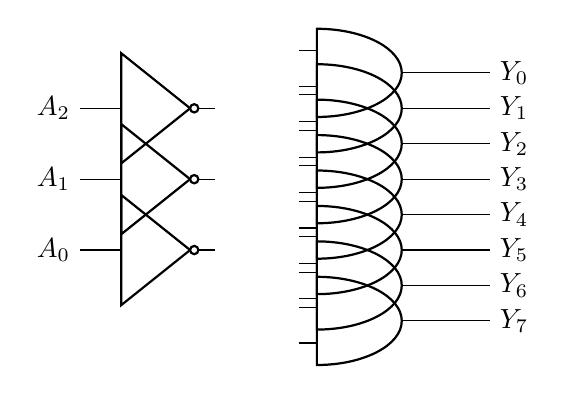
\begin{tikzpicture}[scale=0.9]
  % Input signals
  \node (A2) at (0,1) {$A_2$};
  \node (A1) at (0,0) {$A_1$};
  \node (A0) at (0,-1) {$A_0$};

  % Inverters
  \node[american not port] (inv2) at (1.5,1) {};
  \node[american not port] (inv1) at (1.5,0) {};
  \node[american not port] (inv0) at (1.5,-1) {};

  \draw (A2) -- (inv2.in);
  \draw (A1) -- (inv1.in);
  \draw (A0) -- (inv0.in);

  % AND gates
  \foreach \y in {0,...,7} {
    \node[american and port] (and\y) at (5, 1.5 - 0.5*\y) {};
    \node (Y\y) at (6.5, 1.5 - 0.5*\y) {$Y_\y$};
    \draw (and\y.out) -- (Y\y);
  }
\end{tikzpicture}
\end{center}

\textbf{设计规律}：每个AND门输入端根据该输出的二进制编号选择原变量或反变量。
\begin{itemize}
  \item $Y_5$（101）：$A_2$原变量 $\cdot$ $\overline{A_1}$反变量 $\cdot$ $A_0$原变量
  \item $Y_3$（011）：$\overline{A_2}$反变量 $\cdot$ $A_1$原变量 $\cdot$ $A_0$原变量
\end{itemize}

\textbf{一般规则}：对于 $Y_k$，如果 $k$ 的第 $i$ 位是0，则取 $\overline{A_i}$；如果第 $i$ 位是1，则取 $A_i$。

\section{第六步：为什么这样设计}

\begin{enumerate}
  \item \textbf{为什么每个输出恰好是一个AND门？}

  AND门的特性：\textbf{所有}输入必须为1，输出才为1。译码器的需求恰好是：对于输入组合$(A_2 A_1 A_0)$恰好等于某个特定值时，对应的输出线才为1。AND门天然实现了这个"完全匹配"检测。

  \item \textbf{为什么需要反相器？}

  因为输入信号可能是0。例如：当 $(A_2 A_1 A_0) = 000$ 时，要检测"$A_2=0$且$A_1=0$且$A_0=0$"，必须使用 $\overline{A_2} \cdot \overline{A_1} \cdot \overline{A_0}$ —— 需要三个反相器。

  \item \textbf{译码器与编码器的对偶关系？}

  编码器：输入线号 $\to$ 二进制编码（多对1的OR）
  译码器：二进制编码 $\to$ 输出线号（1对多的AND展开）

  这正是"编码"与"译码"的本质区别。
\end{enumerate}

\section{第七步：考试常见变式}

\begin{enumerate}
  \item \textbf{变式1：低电平有效译码器（如74LS138）}

  输入仍是高电平有效，但输出是低电平有效（选中时输出0，未选中时输出1）。此时将AND门换成NAND门即可，有时输出端还有小圆圈标记。

  74LS138还包含三个使能端：$G_1$（高有效），$\overline{G_{2A}}$和$\overline{G_{2B}}$（低有效）。\textbf{这几乎是必考题！}

  \item \textbf{变式2：用译码器实现任意逻辑函数}

  \textbf{核心考点}：译码器的输出是所有最小项。\textbf{任何组合逻辑函数}都可以表示为若干最小项的OR。

  例如：实现 $F(A,B,C) = \sum m(1,3,5,7)$（即 $F = C$）

  解法：将 $Y_1, Y_3, Y_5, Y_7$ 通过一个OR门连接即可。

  \item \textbf{变式3：用3-8译码器构建4-16译码器}

  使用两片3-8译码器 + 片选信号。高位地址作为片选，选择使用哪一个3-8译码器。

  \item \textbf{变式4：用译码器做地址译码}

  在存储器或外设选择中的应用。n位地址输入，$2^n$个片选信号输出。

  \item \textbf{变式5：显示译码器（BCD-7段译码器）}

  将4位BCD码译为7段数码管的驱动信号。每个输出段也是一个最小项组合的逻辑函数。
\end{enumerate}

\section{第八步：VHDL实现}

\subsection{普通3-8译码器（高电平有效）}

\begin{lstlisting}[caption={3-8译码器（case实现）}]
library ieee;
use ieee.std_logic_1164.all;

entity decoder_3to8 is
  port (
    A : in  std_logic_vector(2 downto 0);
    Y : out std_logic_vector(7 downto 0)
  );
end decoder_3to8;

architecture behavioral of decoder_3to8 is
begin
  process(A)
  begin
    case A is
      when "000" => Y <= "00000001";
      when "001" => Y <= "00000010";
      when "010" => Y <= "00000100";
      when "011" => Y <= "00001000";
      when "100" => Y <= "00010000";
      when "101" => Y <= "00100000";
      when "110" => Y <= "01000000";
      when "111" => Y <= "10000000";
      when others => Y <= "00000000";
    end case;
  end process;
end behavioral;
\end{lstlisting}

\subsection{74LS138风格（低电平有效 + 使能端）}

\begin{lstlisting}[caption={74LS138风格译码器}]
library ieee;
use ieee.std_logic_1164.all;

entity decoder_74ls138 is
  port (
    A  : in  std_logic_vector(2 downto 0);
    G1 : in  std_logic;
    G2A_n : in  std_logic;
    G2B_n : in  std_logic;
    Y_n : out std_logic_vector(7 downto 0)  -- 低电平有效
  );
end decoder_74ls138;

architecture behavioral of decoder_74ls138 is
  signal enable : std_logic;
begin
  enable <= G1 and (not G2A_n) and (not G2B_n);

  process(A, enable)
  begin
    if enable = '0' then
      Y_n <= "11111111";  -- 禁止：所有输出无效
    else
      case A is
        when "000" => Y_n <= "11111110";
        when "001" => Y_n <= "11111101";
        when "010" => Y_n <= "11111011";
        when "011" => Y_n <= "11110111";
        when "100" => Y_n <= "11101111";
        when "101" => Y_n <= "11011111";
        when "110" => Y_n <= "10111111";
        when "111" => Y_n <= "01111111";
        when others => Y_n <= "11111111";
      end case;
    end if;
  end process;
end behavioral;
\end{lstlisting}

\section{第九步：Testbench验证}

\begin{lstlisting}[caption={3-8译码器Testbench}]
library ieee;
use ieee.std_logic_1164.all;

entity decoder_3to8_tb is
end decoder_3to8_tb;

architecture test of decoder_3to8_tb is
  signal A : std_logic_vector(2 downto 0);
  signal Y : std_logic_vector(7 downto 0);

  component decoder_3to8 is
    port (
      A : in  std_logic_vector(2 downto 0);
      Y : out std_logic_vector(7 downto 0)
    );
  end component;
begin
  uut: decoder_3to8 port map (A, Y);

  stimulus: process
  begin
    for i in 0 to 7 loop
      A <= std_logic_vector(to_unsigned(i, 3));
      wait for 10 ns;
    end loop;
    wait;
  end process;
end test;
\end{lstlisting}

\section{第十步：如何快速解题}

\begin{examtip}[译码器快速解题法]
\begin{enumerate}
  \item \textbf{写输出表达式}：$Y_k = \prod A_i^{b_i}$，其中 $b_i$ 是 $k$ 的二进制第 $i$ 位（0取反，1取原）
  \item \textbf{用译码器实现逻辑函数}：将函数表示为最小项之和，将对应输出端用OR门连接
  \item \textbf{级联译码器}：高位地址 $\to$ 片选信号，低位地址 $\to$ 各片译码器的输入
  \item \textbf{有效电平}：高有效用AND，低有效用NAND
\end{enumerate}
\end{examtip}

\textbf{秒杀口诀}：每个输出 = 一个最小项 = 一个AND门（输入原/反变量取决于编号）。

\textbf{最常考：用3-8译码器 + OR门实现任意3变量逻辑函数。}

例子：实现 $F(A,B,C) = \sum m(0,2,4,6)$
解：$F = Y_0 + Y_2 + Y_4 + Y_6$（将四个输出通过OR门连接）

\section{变式详解}
\chapter{3-8译码器——5大变式详解}

\section{变式1：74LS138风格译码器（低有效输出+三使能端）——必考！}

\begin{detailbox}[完整教学]

\textbf{【电路】}
74LS138是考试中最常出现的译码器芯片。特点：
\begin{itemize}
  \item 3位地址输入A2,A1,A0
  \item 8个输出Y0-Y7，\textbf{全部低电平有效}（选中=0，未选中=1）
  \item 3个使能端：G1(高有效), G2A(低有效), G2B(低有效)
  \item 只有三个使能端同时有效（G1=1, G2A=0, G2B=0）时，译码器才工作
\end{itemize}

\textbf{【使能逻辑】}$enable = G1 \cdot \overline{G2A} \cdot \overline{G2B}$

\textbf{【VHDL】}
\begin{lstlisting}
entity decoder_74ls138 is
  port (
    A    : in  std_logic_vector(2 downto 0);
    G1   : in  std_logic;
    G2A_n: in  std_logic;  -- 低有效
    G2B_n: in  std_logic;  -- 低有效
    Y_n  : out std_logic_vector(7 downto 0)  -- 低有效
  );
end decoder_74ls138;

architecture behavioral of decoder_74ls138 is
  signal enable : std_logic;
begin
  enable <= G1 and (not G2A_n) and (not G2B_n);

  process(A, enable)
  begin
    if enable = '0' then
      Y_n <= "11111111";  -- 全高=全无效
    else
      case A is
        when "000" => Y_n <= "11111110";  -- Y0=0
        when "001" => Y_n <= "11111101";  -- Y1=0
        when "010" => Y_n <= "11111011";
        when "011" => Y_n <= "11110111";
        when "100" => Y_n <= "11101111";
        when "101" => Y_n <= "11011111";
        when "110" => Y_n <= "10111111";
        when "111" => Y_n <= "01111111";
        when others => Y_n <= "11111111";
      end case;
    end if;
  end process;
end behavioral;
\end{lstlisting}

\textbf{【为什么用3个使能端】}
多个使能端方便级联。G2A和G2B是低有效，G1是高有效——这种混合设计使得可以用不同信号控制，增加灵活性。

\textbf{【常考陷阱】}
\begin{itemize}
  \item 看清输出是低有效还是高有效——74LS138输出0表示选中
  \item 三个使能端必须\textbf{同时}满足条件译码器才工作
  \item 使能无效时所有输出为1（全高=全无效）
\end{itemize}

\end{detailbox}


\section{变式2：用译码器实现任意逻辑函数（必考！）}

\begin{detailbox}[完整教学]

\textbf{【核心原理】}
译码器的每个输出=一个最小项。\textbf{任何组合逻辑函数}=若干最小项之和（OR）。

\textbf{【通用公式】}$F(A,B,C) = \sum m(\dots)= Y_{i1}+Y_{i2}+Y_{i3}+\dots$

\textbf{【例题】}用3-8译码器+一个OR门实现$F(A,B,C)=\sum m(1,3,5,7)$。

\textbf{【解法】}
\begin{enumerate}
  \item 译码器产生8个最小项：Y0=m0, Y1=m1, ..., Y7=m7
  \item $F = m1+m3+m5+m7 = Y1+Y3+Y5+Y7$
  \item 用1个4输入OR门连接Y1,Y3,Y5,Y7
\end{enumerate}

\textbf{【电路结构】}
\begin{center}
\begin{tikzpicture}
\node[draw,minimum width=2.5cm,minimum height=1.5cm] (dec) at (0,0) {3-8译码器};
\node[american or port] (orgate) at (4,0) {};
\draw[->] (dec.east|-orgate.in 1) -- (orgate.in 1);
\draw[->] (dec.east|-orgate.in 2) -- (orgate.in 2);
\draw[->] (orgate.out) -- ++(1,0) node[right]{$F$};
\node at (0,-2) {A2A1A0 = 变量A,B,C};
\node at (4,-2) {OR门输入=Y1,Y3,Y5,Y7};
\end{tikzpicture}
\end{center}

\textbf{【VHDL】}
\begin{lstlisting}
-- 例化译码器
dec: decoder_3to8 port map(A=>ABC, Y=>Y);
-- OR门
F <= Y(1) or Y(3) or Y(5) or Y(7);
\end{lstlisting}

\textbf{【推广：实现任意3变量函数】}
\begin{center}
\begin{tabular}{|l|l|}
\hline
\textbf{函数} & \textbf{连接} \\
\hline
$F=m0+m2+m4+m6$ & Y0+Y2+Y4+Y6 \\
$F=m0+m1+m2+m3$ & Y0+Y1+Y2+Y3 \\
$F=A$ (即m4+m5+m6+m7) & Y4+Y5+Y6+Y7 \\
$F=\overline{A}$ & Y0+Y1+Y2+Y3 \\
\hline
\end{tabular}
\end{center}

\textbf{【如果函数用NAND实现】}
用NAND门替代OR门（德摩根定理）。此时输出是反相的，但功能等价。

\begin{examfocus}
\textbf{必考！用3-8译码器+门电路实现任意3变量逻辑函数。}
步骤：(1)将函数写成最小项之和 (2)对应Y输出用OR门连接
\end{examfocus}

\end{detailbox}


\section{变式3：用3-8译码器构建4-16译码器（片选级联）}

\begin{detailbox}[完整教学]

\textbf{【问题】}只有3-8译码器，如何得到4位地址→16个输出的4-16译码器？

\textbf{【方案】}两片3-8译码器+最高位地址A3做片选。

\textbf{【级联逻辑】}
\begin{itemize}
  \item \textbf{片0（低位）}：处理A3=0时，地址0000-0111（译码器输出Y0-Y7对应系统Y0-Y7）
  \item \textbf{片1（高位）}：处理A3=1时，地址1000-1111（译码器输出Y0-Y7对应系统Y8-Y15）
  \item A3=0→片0使能，片1禁止
  \item A3=1→片1使能，片0禁止
\end{itemize}

\textbf{【VHDL】}
\begin{lstlisting}
entity decoder_4to16 is
  port (A : in std_logic_vector(3 downto 0);
        Y : out std_logic_vector(15 downto 0));
end decoder_4to16;

architecture structural of decoder_4to16 is
  signal Y_low, Y_high : std_logic_vector(7 downto 0);
  component decoder_3to8 is
    port (A : in std_logic_vector(2 downto 0);
          E : in std_logic; Y : out std_logic_vector(7 downto 0));
  end component;
begin
  -- 片0：A3=0时使能
  dec_low: decoder_3to8 port map(
    A => A(2 downto 0), E => not A(3), Y => Y_low);

  -- 片1：A3=1时使能
  dec_high: decoder_3to8 port map(
    A => A(2 downto 0), E => A(3), Y => Y_high);

  Y <= Y_high & Y_low;  -- 拼接为16位输出
end structural;
\end{lstlisting}

\textbf{【通用级联公式】}
用$2^k$个$n$-$2^n$译码器构建$(n+k)$-$2^{n+k}$译码器。
高k位地址→片选，低n位地址→各片输入。

\textbf{【常见考题】}用两片74LS138构建4-16译码器。利用使能端做片选。

\end{detailbox}


\section{变式4：用译码器做地址译码}

\begin{detailbox}[完整教学]

\textbf{【应用场景】}
CPU有16位地址总线，但连接了多个外设（RAM、ROM、IO端口等）。
用译码器将地址空间划分为不同区域，产生各外设的片选信号。

\textbf{【例题】}用3-8译码器产生8个外设的片选信号。地址A15-A13做译码输入。

\textbf{【电路】}
\begin{center}
\begin{tabular}{|c|c|l|}
\hline
A15A14A13 & 选中输出 & 外设 \\
\hline
000 & Y0 & RAM1(0x0000-0x1FFF) \\
001 & Y1 & RAM2(0x2000-0x3FFF) \\
010 & Y2 & ROM (0x4000-0x5FFF) \\
011 & Y3 & IO1 (0x6000-0x7FFF) \\
100 & Y4 & IO2 (0x8000-0x9FFF) \\
\hline
\end{tabular}
\end{center}

\textbf{【核心思想】}高位地址→译码→片选。低位地址→片内寻址。

\end{detailbox}


\section{变式5：显示译码器（BCD→7段）}

\begin{detailbox}[完整教学]

\textbf{【问题】}3-8译码器每次只选中1个输出。但7段数码管需要同时点亮多个段（如数字"8"需要7段全亮）。

\textbf{【区别】}
\begin{itemize}
  \item 3-8译码器：$n$输入→$2^n$输出，输出是\textbf{互斥}的（恰好一个为1）
  \item BCD-7段译码器：4输入→7输出，输出\textbf{不互斥}（可以同时多个为1）
\end{itemize}

\textbf{【详见第三章BCD译码器】}BCD-7段译码器本质上是7个独立的组合逻辑函数，不是简单的"最小项展开"。

\begin{examfocus}
\textbf{关键区别}：
\begin{itemize}
  \item 3-8译码器：1-of-N选择（互斥输出）→ 用AND门
  \item BCD-7段：任意多段同时亮（非互斥）→ 用ROM/查找表
\end{itemize}
不搞混这两种"译码器"是考试的基本要求。
\end{examfocus}

\end{detailbox}


\section{译码器变式总结}

\begin{examfocus}[译码器5大变式速查]
\begin{center}
\begin{tabular}{|l|l|l|}
\hline
\textbf{变式} & \textbf{核心考点} & \textbf{常考题型} \\
\hline
74LS138风格 & 低有效+3使能端 & 写VHDL, 判断使能条件 \\
译码器+OR≈任意函数 & 最小项之和 & 给定函数→画电路 \\
级联构建更大译码器 & 高位地址做片选 & 74LS138×2→4-16 \\
地址译码 & 地址空间划分 & 存储器片选设计 \\
vs BCD-7段 & 互斥vs非互斥输出 & 概念辨析 \\
\hline
\end{tabular}
\end{center}
\end{examfocus}

\chapter{BCD译码器}

\section{第一步：解决什么问题}

计算机内部使用二进制运算，但人类需要看到十进制数字。

\textbf{问题}：FPGA内部计算结果是4位二进制（0000到1111），如何在7段数码管上显示为人类可读的十进制数字（0到9）？

\textbf{方案}：将4位BCD码（Binary-Coded Decimal）转换为7段数码管的驱动信号。

BCD码：用4位二进制数表示一个十进制数字。

\begin{itemize}
  \item 0 $\to$ 0000
  \item 1 $\to$ 0001
  \item 2 $\to$ 0010
  \item ...
  \item 9 $\to$ 1001
\end{itemize}

注意：1010到1111（10到15）在BCD中是非法的，不应出现。

\section{第二步：输入输出关系}

\begin{itemize}
  \item \textbf{输入}：$A_3, A_2, A_1, A_0$（4位BCD码，表示0-9）
  \item \textbf{输出}：$a, b, c, d, e, f, g$（7段，每一段控制数码管的一段LED）
\end{itemize}

7段数码管的段命名：

\begin{center}
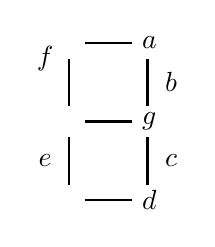
\begin{tikzpicture}[scale=1.0]
  % 7-segment display with segment labels
  \draw[thick] (0,2) -- (0.6,2) node[right] {$a$};  % top
  \draw[thick] (0.8,1.2) -- (0.8,1.8);              % top-right: b
  \draw[thick] (0.8,0.2) -- (0.8,0.8);              % bottom-right: c
  \draw[thick] (0,0) -- (0.6,0) node[right] {$d$};  % bottom
  \draw[thick] (-0.2,0.2) -- (-0.2,0.8);            % bottom-left: e
  \draw[thick] (-0.2,1.2) -- (-0.2,1.8);            % top-left: f
  \draw[thick] (0,1) -- (0.6,1) node[right] {$g$};  % middle
  \node at (-0.5,1.8) {$f$};
  \node at (1.1,1.5) {$b$};
  \node at (-0.5,0.5) {$e$};
  \node at (1.1,0.5) {$c$};
\end{tikzpicture}
\end{center}

\section{第三步：真值表}

\begin{center}
\small
\begin{tabular}{|c|c|c|c||c|c|c|c|c|c|c||c|}
\hline
$A_3$ & $A_2$ & $A_1$ & $A_0$ & $a$ & $b$ & $c$ & $d$ & $e$ & $f$ & $g$ & 显示 \\
\hline
0 & 0 & 0 & 0 & 1 & 1 & 1 & 1 & 1 & 1 & 0 & 0 \\
0 & 0 & 0 & 1 & 0 & 1 & 1 & 0 & 0 & 0 & 0 & 1 \\
0 & 0 & 1 & 0 & 1 & 1 & 0 & 1 & 1 & 0 & 1 & 2 \\
0 & 0 & 1 & 1 & 1 & 1 & 1 & 1 & 0 & 0 & 1 & 3 \\
0 & 1 & 0 & 0 & 0 & 1 & 1 & 0 & 0 & 1 & 1 & 4 \\
0 & 1 & 0 & 1 & 1 & 0 & 1 & 1 & 0 & 1 & 1 & 5 \\
0 & 1 & 1 & 0 & 1 & 0 & 1 & 1 & 1 & 1 & 1 & 6 \\
0 & 1 & 1 & 1 & 1 & 1 & 1 & 0 & 0 & 0 & 0 & 7 \\
1 & 0 & 0 & 0 & 1 & 1 & 1 & 1 & 1 & 1 & 1 & 8 \\
1 & 0 & 0 & 1 & 1 & 1 & 1 & 1 & 0 & 1 & 1 & 9 \\
\hline
\end{tabular}
\end{center}

对于1010到1111（10-15），输出通常全部熄灭（全0）或显示特定模式（取决于设计）。

\section{第四步：逻辑推导}

每一段都是一个4变量组合逻辑函数。以$a$段为例：

$a = 1$ 当输入为：0(0000), 2(0010), 3(0011), 5(0101), 6(0110), 7(0111), 8(1000), 9(1001)

即：$a = \sum m(0,2,3,5,6,7,8,9)$

卡诺图化简后（此处省略卡诺图步骤，这是我们有意跳过的部分），得到：

\begin{align}
  a &= A_3 + A_1 + \overline{A_2}\cdot\overline{A_0} + A_2\cdot A_0 \\
  b &= \overline{A_2} + \overline{A_1}\cdot\overline{A_0} + A_1\cdot A_0 \\
  c &= \overline{A_1} + A_0 + A_2 \\
  d &= \overline{A_2}\cdot\overline{A_0} + A_1\cdot\overline{A_0} + \overline{A_2}\cdot A_1 + A_2\cdot\overline{A_1}\cdot A_0 \\
  e &= \overline{A_2}\cdot\overline{A_0} + A_1\cdot\overline{A_0} \\
  f &= A_3 + \overline{A_1}\cdot\overline{A_0} + A_2\cdot\overline{A_1} + A_2\cdot\overline{A_0} \\
  g &= A_3 + \overline{A_2}\cdot A_1 + A_1\cdot\overline{A_0} + A_2\cdot\overline{A_1}
\end{align}

但在考试中，\textbf{你不会也不需要手算这些表达式}。考试更可能考的是理解BCD译码器的功能和使用方法。

\section{第五步：结构化设计}

BCD-7段译码器 = 7个4变量组合逻辑函数，每个函数通过ROM/查找表实现：

\begin{center}
\begin{tikzpicture}
  \node[draw, minimum width=3cm, minimum height=4cm] (rom) at (0,0) {ROM/查找表};
  \node (A) at (-3,1) {$A_{3:0}$};
  \node (seg) at (3,1) {$a,b,c,d,e,f,g$};
  \draw[->] (A) -- (rom.west |- A);
  \draw[->] (rom.east |- seg) -- (seg);
  \node at (0,-3) {输入：4位BCD → 查表 → 输出：7段控制信号};
\end{tikzpicture}
\end{center}

\section{第六步：为什么这样设计}

\begin{enumerate}
  \item \textbf{为什么用查找表而非单独的门电路？}

  7段译码器涉及7个4变量函数。如果每个都用门电路实现，需要大量AND门和OR门。使用ROM（16×7 = 112 bits）更简洁，这也是FPGA中LUT（查找表）的实际实现方式。

  \item \textbf{为什么1010-1111是非法输入？}

  BCD码的定义：4位二进制只使用前10个编码（0000-1001）。后6个编码（1010-1111）不表示任何十进制数字，是非法BCD码。好的设计应该对所有输入都定义行为（全部熄灭或显示异常标记）。

  \item \textbf{与普通3-8译码器的本质区别？}

  3-8译码器：每个输出是\textbf{一个}最小项（3输入AND）
  BCD-7段译码器：每个输出是\textbf{多个}最小项之和（4输入的组合逻辑函数）

  所以BCD-7段译码器本质上是7个独立的组合逻辑函数。
\end{enumerate}

\section{第七步：考试常见变式}

\begin{enumerate}
  \item \textbf{变式1：多位BCD显示}

  多个BCD译码器 + 多个7段数码管，实现多位数显示。通常配合动态扫描技术（快速轮流点亮各数码管，利用人眼视觉暂留）。

  \item \textbf{变式2：带锁存功能的BCD译码器}

  输入锁存：在LE（Latch Enable）信号控制下锁存当前BCD输入，数码管保持显示不变。这在需要稳定显示时非常有用。

  \item \textbf{变式3：共阳极 vs 共阴极数码管}

  共阳极：所有LED阳极接一起（接VCC），段驱动需要低电平点亮（输出0 = 亮）
  共阴极：所有LED阴极接一起（接GND），段驱动需要高电平点亮（输出1 = 亮）

  两种类型的输出值恰好互为反码。

  \item \textbf{变式4：计数 + 显示系统}

  这是考试常见综合题：计数器产生BCD码 $\to$ BCD译码器 $\to$ 7段数码管显示。考察对整个数字系统流程的理解。

  \item \textbf{变式5：16进制显示译码器}

  输入0-15（全4位二进制），输出0-9 + A-F。比BCD译码器多6个有效输入状态。
\end{enumerate}

\section{第八步：VHDL实现}

\begin{lstlisting}[caption={BCD-7段译码器（case版本）}]
library ieee;
use ieee.std_logic_1164.all;

entity bcd_7seg is
  port (
    bcd : in  std_logic_vector(3 downto 0);
    seg : out std_logic_vector(6 downto 0)  -- a,b,c,d,e,f,g
  );
end bcd_7seg;

architecture behavioral of bcd_7seg is
begin
  process(bcd)
  begin
    case bcd is
      when "0000" => seg <= "1111110";  -- 0
      when "0001" => seg <= "0110000";  -- 1
      when "0010" => seg <= "1101101";  -- 2
      when "0011" => seg <= "1111001";  -- 3
      when "0100" => seg <= "0110011";  -- 4
      when "0101" => seg <= "1011011";  -- 5
      when "0110" => seg <= "1011111";  -- 6
      when "0111" => seg <= "1110000";  -- 7
      when "1000" => seg <= "1111111";  -- 8
      when "1001" => seg <= "1111011";  -- 9
      when others => seg <= "0000000";  -- 全灭
    end case;
  end process;
end behavioral;
\end{lstlisting}

\section{第九步：Testbench验证}

\begin{lstlisting}[caption={BCD-7段译码器Testbench}]
library ieee;
use ieee.std_logic_1164.all;

entity bcd_7seg_tb is
end bcd_7seg_tb;

architecture test of bcd_7seg_tb is
  signal bcd : std_logic_vector(3 downto 0);
  signal seg : std_logic_vector(6 downto 0);

  component bcd_7seg is
    port (
      bcd : in  std_logic_vector(3 downto 0);
      seg : out std_logic_vector(6 downto 0)
    );
  end component;
begin
  uut: bcd_7seg port map (bcd, seg);

  stimulus: process
  begin
    for i in 0 to 15 loop
      bcd <= std_logic_vector(to_unsigned(i, 4));
      wait for 10 ns;
    end loop;
    wait;
  end process;
end test;
\end{lstlisting}

\section{第十步：如何快速解题}

\begin{examtip}[BCD译码器快速解题法]
\begin{enumerate}
  \item \textbf{case实现是标准答案}：在VHDL中用case列举10个有效输入，不需要推导门级表达式
  \item \textbf{注意有效电平}：共阳极（0亮）vs共阴极（1亮），输出值互为反码
  \item \textbf{非法输入处理}：1010-1111用when others，全灭或显示特定标记
  \item \textbf{综合题}：计数器+译码器+数码管 = 经典考试题
\end{enumerate}
\end{examtip}

\section{变式详解}
\chapter{BCD译码器——5大变式详解}

\section{变式1：多位BCD动态扫描显示}

\begin{detailbox}[完整教学]
\textbf{【问题】}4位数码管需要4个BCD-7段译码器吗？如果每个译码器单独驱动→需要4×7=28个IO口。

\textbf{【方案】}动态扫描：1个译码器驱动所有数码管的段，快速轮流点亮各数码管（>50Hz），利用人眼视觉暂留。

\textbf{【电路】}
计数器→2-4译码器→轮流选通4个数码管的共阴/共阳极。BCD译码器输出段码到所有数码管。

\textbf{【VHDL核心逻辑】}
\begin{lstlisting}
process(clk)  -- 扫描时钟(通常>200Hz)
begin
  if rising_edge(clk) then
    scan_cnt <= scan_cnt + 1;
    case scan_cnt is
      when "00" => digit_sel <= "0001"; seg_data <= digit0;
      when "01" => digit_sel <= "0010"; seg_data <= digit1;
      when "10" => digit_sel <= "0100"; seg_data <= digit2;
      when "11" => digit_sel <= "1000"; seg_data <= digit3;
    end case;
  end if;
end process;
\end{lstlisting}

\textbf{【常见考题】}设计4位动态扫描显示电路。
\end{detailbox}


\section{变式2：带锁存的BCD译码器}

\begin{detailbox}[完整教学]
\textbf{【问题】}BCD译码器输入随时钟快速变化→数码管闪烁。需要"定格"显示。

\textbf{【方案】}在译码器前加寄存器。LE=1时锁存当前BCD值，LE=0时保持上次锁存值不变。

\textbf{【VHDL】}
\begin{lstlisting}
process(clk)
begin
  if rising_edge(clk) then
    if LE = '1' then
      latched_bcd <= bcd_input;  -- 锁存
    end if;
  end if;
end process;
seg <= bcd_to_7seg(latched_bcd);  -- 译码锁存后的值
\end{lstlisting}

\textbf{【设计思想】}锁存=寄存器=1个时钟沿保存数据。本质=在数据通路上插入一级寄存器。
\end{detailbox}


\section{变式3：共阳极 vs 共阴极数码管}

\begin{detailbox}[完整教学]
\textbf{【共阳极】}所有LED阳极接VCC。段驱动需低电平(0)点亮LED。seg='0'=亮。
\textbf{【共阴极】}所有LED阴极接GND。段驱动需高电平(1)点亮LED。seg='1'=亮。

\textbf{【输出值关系】}$seg_{\text{共阳}} = \text{not } seg_{\text{共阴}}$（互为反码）

\textbf{【VHDL适配】}
\begin{lstlisting}
-- 共阴极(1亮)
when "0000" => seg <= "1111110";  -- 0
-- 共阳极(0亮)
when "0000" => seg <= "0000001";  -- 0(反码)
\end{lstlisting}

\textbf{【考试陷阱】}题目未明确说明共阴/共阳时，看段码值判断：1111110(共阴0) vs 0000001(共阳0)。
\end{detailbox}


\section{变式4：计数器+译码器+数码管——综合题}

\begin{detailbox}[完整教学]
\textbf{【经典考题】}设计0-9计数器+BCD-7段译码器+数码管显示。

\textbf{【完整VHDL】}
\begin{lstlisting}
entity counter_display is
  port (clk, rst_n : in std_logic;
        seg : out std_logic_vector(6 downto 0));
end counter_display;

architecture rtl of counter_display is
  signal cnt : std_logic_vector(3 downto 0);
  function bcd7seg(bcd : std_logic_vector(3 downto 0))
    return std_logic_vector is
  begin
    case bcd is
      when "0000" => return "1111110";
      when "0001" => return "0110000";
      when "0010" => return "1101101";
      when "0011" => return "1111001";
      when "0100" => return "0110011";
      when "0101" => return "1011011";
      when "0110" => return "1011111";
      when "0111" => return "1110000";
      when "1000" => return "1111111";
      when "1001" => return "1111011";
      when others => return "0000000";
    end case;
  end function;
begin
  process(clk, rst_n)
  begin
    if rst_n='0' then cnt <= "0000";
    elsif rising_edge(clk) then
      if cnt = "1001" then cnt <= "0000";
      else cnt <= cnt + 1;
      end if;
    end if;
  end process;
  seg <= bcd7seg(cnt);
end rtl;
\end{lstlisting}

\textbf{【考点】}两个模块整合：计数器+译码器。
\end{detailbox}


\section{变式5：16进制显示译码器（0-F）}

\begin{detailbox}[完整教学]
\textbf{【问题】}BCD译码器只显示0-9。如何显示0-F（全4位二进制）？

\textbf{【方案】}扩展case覆盖1010-1111，定义A-F的段码。

\begin{lstlisting}
-- 扩展BCD译码器支持0-F
when "1010" => return "1110111";  -- A
when "1011" => return "0011111";  -- b
when "1100" => return "1001110";  -- C
when "1101" => return "0111101";  -- d
when "1110" => return "1001111";  -- E
when "1111" => return "1000111";  -- F
\end{lstlisting}

\textbf{【考试】}有时问A-F的段码值，需要记住典型表示法。
\end{detailbox}

\chapter{4选1数据选择器（MUX）}

\section{第一步：解决什么问题}

想象一个场景：你需要从4个数据源中选择1个传给后续电路。

\begin{itemize}
  \item 不是同时传4个——那需要4条数据通路
  \item 而是：用2根选择线指定"要哪一个"，1根数据线输出
\end{itemize}

\begin{keypoint}[MUX的本质]
数据选择器（Multiplexer, MUX）= 一个受控的多路开关

$2^n$ 个数据输入 $\to$ $n$ 条选择线 $\to$ 1个输出

选择线决定"哪一路数据通向输出"
\end{keypoint}

\section{第二步：输入输出关系}

4选1 MUX：

\begin{itemize}
  \item \textbf{数据输入}：$D_0, D_1, D_2, D_3$
  \item \textbf{选择输入}：$S_1, S_0$（2位，选择哪个数据输入）
  \item \textbf{输出}：$Y$
  \item \textbf{功能}：$Y = D_{(S_1 S_0)}$
\end{itemize}

\section{第三步：真值表}

\begin{center}
\begin{tabular}{|c|c||c|}
\hline
$S_1$ & $S_0$ & $Y$ \\
\hline
0 & 0 & $D_0$ \\
0 & 1 & $D_1$ \\
1 & 0 & $D_2$ \\
1 & 1 & $D_3$ \\
\hline
\end{tabular}
\end{center}

\section{第四步：逻辑推导}

从真值表可以写出：

\begin{equation}
  Y = \overline{S_1} \cdot \overline{S_0} \cdot D_0
    + \overline{S_1} \cdot S_0 \cdot D_1
    + S_1 \cdot \overline{S_0} \cdot D_2
    + S_1 \cdot S_0 \cdot D_3
\end{equation}

\textbf{关键观察}：MUX的每个选择组合对应一个\textbf{乘积项}。

\begin{itemize}
  \item 选择线产生最小项（$\overline{S_1}\cdot\overline{S_0}$, $\overline{S_1}\cdot S_0$等）
  \item 每个数据输入与其对应的最小项AND
  \item 所有结果OR起来
\end{itemize}

\section{第五步：结构化设计}

4选1 MUX内部结构 = 4个3输入AND门 + 1个4输入OR门 + 2个反相器：

\begin{center}
\begin{tikzpicture}[scale=0.85]
  % Inputs
  \node (D0) at (-4,3) {$D_0$};
  \node (D1) at (-4,1) {$D_1$};
  \node (D2) at (-4,-1) {$D_2$};
  \node (D3) at (-4,-3) {$D_3$};
  \node (S1) at (-4,-5) {$S_1$};
  \node (S0) at (-4,-6) {$S_0$};

  % Internal structure is complex, using simplified representation
  \node[draw, minimum width=4cm, minimum height=5cm,
        label=above:MUX 4选1] (mux) at (0,0) {};

  \node (Y) at (3,0) {$Y$};
  \draw[->] (mux.east) -- (Y);

  % Selection notation
  \node at (0,-3.5) {\small $S_1S_0$};
\end{tikzpicture}
\end{center}

\section{第六步：为什么这样设计}

\begin{enumerate}
  \item \textbf{为什么MUX是"万能"的组合逻辑？}

  因为MUX输出 = $\sum$（选择最小项 $\cdot$ 数据输入）。

  如果把数据输入当作"该最小项是否参与"的控制：
  \begin{itemize}
    \item $D_k = 1$：该最小项参与（函数包含此最小项）
    \item $D_k = 0$：该最小项不参与
  \end{itemize}

  所以：\textbf{任何$n$变量逻辑函数都可以用一个$2^n$选1 MUX实现}！

  只需将函数真值表的输出列接到MUX的数据输入端。

  \item \textbf{为什么MUX能节省资源？}

  将"多路数据"变成"一路分时复用"——不需要为每路数据各建一条独立通路。这是时分复用的基本思想。

  \item \textbf{MUX与译码器的关系？}

  译码器产生所有$2^n$个最小项（$n$输入$\to$$2^n$输出），MUX选择其中一个输出。实际上，MUX = 译码器 + AND-OR结构。
\end{enumerate}

\section{第七步：考试常见变式}

\begin{enumerate}
  \item \textbf{变式1：用MUX实现任意逻辑函数（必考！）}

  \textbf{方法}：将函数的变量接选择线，真值表的输出值接数据输入。

  例：实现 $F(A,B,C) = \sum m(0,1,4,6,7)$

  用8选1 MUX：$D_0=1, D_1=1, D_2=0, D_3=0, D_4=1, D_5=0, D_6=1, D_7=1$

  \textbf{降维技巧}：用$2^{n-1}$选1 MUX实现$n$变量函数

  选择线只接$n-1$个变量，第$n$个变量（或其反变量）接到某些数据输入端。

  例：用4选1 MUX实现3变量函数 $F(A,B,C)$

  将A,B接选择线 $S_1,S_0$，C（或其反）接到某些数据输入端。

  \item \textbf{变式2：双4选1 MUX（8选1功能）}

  两片4选1 MUX + 一片2选1 MUX = 8选1 MUX。

  \item \textbf{变式3：带使能端的MUX}

  使能端E=0时，输出固定为0（或高阻态），无论选择线是什么。

  \item \textbf{变式4：MUX扩展}

  $n$选1 MUX可以通过级联构建更大的MUX。例如：4片4选1 MUX + 1片4选1 MUX = 16选1 MUX。
\end{enumerate}

\section{第八步：VHDL实现}

\begin{lstlisting}[caption={4选1 MUX（多种实现方式）}]
-- 方式1: with-select (最简洁)
architecture with_select of mux4to1 is
begin
  with S select
    Y <= D(0) when "00",
         D(1) when "01",
         D(2) when "10",
         D(3) when "11",
         '0'   when others;
end with_select;

-- 方式2: when-else (条件信号赋值)
architecture when_else of mux4to1 is
begin
  Y <= D(0) when S = "00" else
       D(1) when S = "01" else
       D(2) when S = "10" else
       D(3) when S = "11" else
       '0';
end when_else;

-- 方式3: process + case
architecture proc_case of mux4to1 is
begin
  process(S, D)
  begin
    case S is
      when "00" => Y <= D(0);
      when "01" => Y <= D(1);
      when "10" => Y <= D(2);
      when "11" => Y <= D(3);
      when others => Y <= '0';
    end case;
  end process;
end proc_case;
\end{lstlisting}

\begin{lstlisting}[caption={完整4选1 MUX实体}]
library ieee;
use ieee.std_logic_1164.all;

entity mux4to1 is
  port (
    D : in  std_logic_vector(3 downto 0);
    S : in  std_logic_vector(1 downto 0);
    Y : out std_logic
  );
end mux4to1;
\end{lstlisting}

\section{第九步：Testbench验证}

\begin{lstlisting}[caption={4选1 MUX Testbench}]
library ieee;
use ieee.std_logic_1164.all;

entity mux4to1_tb is
end mux4to1_tb;

architecture test of mux4to1_tb is
  signal D : std_logic_vector(3 downto 0);
  signal S : std_logic_vector(1 downto 0);
  signal Y : std_logic;

  component mux4to1 is
    port (
      D : in  std_logic_vector(3 downto 0);
      S : in  std_logic_vector(1 downto 0);
      Y : out std_logic
    );
  end component;
begin
  uut: mux4to1 port map (D, S, Y);

  stimulus: process
  begin
    D <= "1010";  -- 固定数据输入
    S <= "00"; wait for 10 ns;  -- Y = D0 = 0
    S <= "01"; wait for 10 ns;  -- Y = D1 = 1
    S <= "10"; wait for 10 ns;  -- Y = D2 = 0
    S <= "11"; wait for 10 ns;  -- Y = D3 = 1
    wait;
  end process;
end test;
\end{lstlisting}

\section{第十步：如何快速解题}

\begin{examtip}[MUX快速解题法]
\begin{enumerate}
  \item \textbf{用MUX实现逻辑函数}：真值表的输出列 = MUX的数据输入列（这是最快的做法）
  \item \textbf{降维法}：$n$变量函数 $\to$ 用$2^{n-1}$选1 MUX。剩余的1个变量（或其反）接数据输入
  \item \textbf{级联扩展}：小MUX + 小MUX = 大MUX
  \item \textbf{VHDL}：with-select 是最简洁的MUX写法，综合结果就是MUX硬件
\end{enumerate}
\end{examtip}

\textbf{秒杀必考题：用MUX实现逻辑函数}

\noindent 题：用8选1 MUX实现 $F(A,B,C) = \sum m(0, 3, 5, 6)$

\noindent 解：$D_0=1, D_1=0, D_2=0, D_3=1, D_4=0, D_5=1, D_6=1, D_7=0$

\section{变式详解}
\chapter{4选1 MUX——4大变式详解}

\section{变式1：用MUX实现任意逻辑函数（必考！）}

\begin{detailbox}[完整教学]
\textbf{【核心原理】}
MUX的通用表达式：$Y=\overline{S_1}\cdot\overline{S_0}\cdot D_0+\overline{S_1}\cdot S_0\cdot D_1+S_1\cdot\overline{S_0}\cdot D_2+S_1\cdot S_0\cdot D_3$

如果把$S_1,S_0$接函数变量，$D_k$接"该最小项是否参与=1"：$D_k$接1→该最小项参与函数。$D_k$接0→不参与。

\textbf{【结论】任何n变量逻辑函数=一个$2^n$选1 MUX}

\textbf{【例题1】}用8选1 MUX实现$F(A,B,C)=\sum m(0,3,5,6)$

\textbf{解：}$D_0=1,D_1=0,D_2=0,D_3=1,D_4=0,D_5=1,D_6=1,D_7=0$

将m0-m7对应的D分别接1或0。选择线S2,S1,S0接A,B,C。

\textbf{【例题2：降维法】}用4选1 MUX实现3变量函数$F(A,B,C)=\sum m(0,1,4,6,7)$

$2^{3-1}=4$选1 MUX, 变量A,B接S1,S0, C用于产生$D_k$。

\begin{center}
\begin{tabular}{|c|c|c|c|c|}
\hline
AB & m(C=0) & m(C=1) & D输入 & 逻辑 \\
\hline
00 & m0=1 & m1=1 & D0 & 1(与C无关) \\
01 & m2=0 & m3=0 & D1 & 0 \\
10 & m4=1 & m5=0 & D2 & $\overline{C}$ \\
11 & m6=1 & m7=1 & D3 & 1 \\
\hline
\end{tabular}
\end{center}

D0=1, D1=0, D2=$\overline{C}$, D3=1.

\textbf{【VHDL】}
\begin{lstlisting}
entity mux_logic is
  port (A, B, C : in std_logic; F : out std_logic);
end mux_logic;
architecture rtl of mux_logic is
  signal D : std_logic_vector(3 downto 0);
  signal S : std_logic_vector(1 downto 0);
begin
  S <= A & B;
  D <= '1' & (not C) & '0' & '1';  -- D3,D2,D1,D0
  with S select F <=
    D(0) when "00", D(1) when "01",
    D(2) when "10", D(3) when "11";
end rtl;
\end{lstlisting}

\begin{examfocus}
\textbf{这是组合逻辑的必考题！}两种考法：
(1) $2^n$选1 MUX实现n变量函数 → Dk直接接0/1
(2) $2^{n-1}$选1 MUX实现n变量函数 → 需要降维，剩余变量或其反接到D端
\end{examfocus}
\end{detailbox}


\section{变式2：双4选1 MUX构建8选1 MUX}

\begin{detailbox}[完整教学]
\textbf{【结构】}两片4选1 MUX处理低2位地址。一片2选1 MUX用最高位地址S2选择输出。
总MUX数：3片(2×4选1 + 1×2选1)。

\textbf{【VHDL——结构级】}
\begin{lstlisting}
-- 片0：S1S0选D0-D3
mux_low: entity work.mux4to1 port map(D=>D(3 downto 0), S=>S(1 downto 0), Y=>F_low);
-- 片1：S1S0选D4-D7
mux_high: entity work.mux4to1 port map(D=>D(7 downto 4), S=>S(1 downto 0), Y=>F_high);
-- 顶层2选1
F <= F_low when S(2)='0' else F_high;
\end{lstlisting}
\end{detailbox}


\section{变式3：带使能端的MUX}

\begin{detailbox}[完整教学]
\textbf{【功能】}E=1正常选择；E=0输出高阻态'Z'（三态输出）或固定'0'。

\textbf{【VHDL——三态输出】}
\begin{lstlisting}
F <= D(to_integer(unsigned(S))) when E='1' else 'Z';
\end{lstlisting}

\textbf{【应用】}多个MUX输出可共用一根总线（总线仲裁）。
\end{detailbox}


\section{变式4：MUX扩展——16选1}

\begin{detailbox}[完整教学]
\textbf{【树形结构】}4片4选1 MUX(第一层)+1片4选1 MUX(第二层)=16选1。
总MUX数：5片。

\textbf{【选择位分配】}S1S0→第一层(4片)，S3S2→第二层(1片)。
\end{detailbox}

\chapter{4位数据比较器}

\section{第一步：解决什么问题}

比较两个二进制数的大小关系。

这是数字系统中非常基础的操作：CPU的跳转指令（BEQ, BNE, BLT, BGT）本质上就是在做数值比较。

\begin{keypoint}[比较器的本质]
比较器 = 判断 $A$ 和 $B$ 的大小关系

三个输出：$A>B$、$A=B$、$A<B$（互斥，任意时刻恰好一个为1）
\end{keypoint}

\section{第二步：输入输出关系}

4位比较器：

\begin{itemize}
  \item \textbf{数据输入}：$A_3 A_2 A_1 A_0$（4位），$B_3 B_2 B_1 B_0$（4位）
  \item \textbf{级联输入}：$I_{A>B}, I_{A=B}, I_{A<B}$（用于级联多片比较器）
  \item \textbf{输出}：$Y_{A>B}, Y_{A=B}, Y_{A<B}$
\end{itemize}

\section{第三步：比较逻辑}

比较两个多位二进制数的方法：\textbf{从高位到低位逐位比较}。

\begin{enumerate}
  \item 先看最高位（MSB）$A_3$ vs $B_3$
  \begin{itemize}
    \item 如果 $A_3 > B_3$（即 $A_3=1, B_3=0$），则 $A > B$，\textbf{比较结束}
    \item 如果 $A_3 < B_3$（即 $A_3=0, B_3=1$），则 $A < B$，\textbf{比较结束}
    \item 如果 $A_3 = B_3$，则 \textbf{继续看下一位}
  \end{itemize}
  \item 然后看 $A_2$ vs $B_2$（同上逻辑）
  \item 然后看 $A_1$ vs $B_1$
  \item 最后看 $A_0$ vs $B_0$
\end{enumerate}

\textbf{这完全类比人类比较两个数字的方法}：先看最高位，相等再看次高位。

\section{第四步：逻辑推导}

一位比较器的基本单元：

\begin{itemize}
  \item $A_i > B_i$：$A_i \cdot \overline{B_i}$
  \item $A_i < B_i$：$\overline{A_i} \cdot B_i$
  \item $A_i = B_i$：$\overline{A_i \oplus B_i}$ （XNOR）
\end{itemize}

多位比较器 = 从高位到低位的级联比较：

\begin{align}
  A>B &= (A_3 > B_3) + (A_3 = B_3) \cdot (A_2 > B_2) \\
      &\quad + (A_3 = B_3) \cdot (A_2 = B_2) \cdot (A_1 > B_1) \nonumber \\
      &\quad + (A_3 = B_3) \cdot (A_2 = B_2) \cdot (A_1 = B_1) \cdot (A_0 > B_0) \nonumber
\end{align}

即：在更高位全部相等的前提下，看当前位谁大谁小。

\begin{align}
  A=B &= (A_3 = B_3) \cdot (A_2 = B_2) \cdot (A_1 = B_1) \cdot (A_0 = B_0) \\
  A<B &= \text{（对称逻辑）}
\end{align}

\section{第五步：结构化设计}

比较器内部结构 = 逐位比较单元 + 优先级逻辑：

\begin{center}
\begin{tikzpicture}
  % MSB comparison
  \node[draw, minimum width=2cm, minimum height=1.5cm] (cmp3) at (0,3) {bit3比较};
  \node[draw, minimum width=2cm, minimum height=1.5cm] (cmp2) at (0,2) {bit2比较};
  \node[draw, minimum width=2cm, minimum height=1.5cm] (cmp1) at (0,1) {bit1比较};
  \node[draw, minimum width=2cm, minimum height=1.5cm] (cmp0) at (0,0) {bit0比较};

  % Priority chain
  \draw[->] (cmp3.east) -- ++(0.5,0) |- (2,2.5) node[right] {若相等则};
  \draw[->] (cmp2.east) -- ++(0.5,0) |- (2,1.5) node[right] {若相等则};
  \draw[->] (cmp1.east) -- ++(0.5,0) |- (2,0.5) node[right] {若相等则};
\end{tikzpicture}
\end{center}

\textbf{关键设计思想}：优先级从高到低。高位比较的结果优先级最高。

\section{第六步：为什么这样设计}

\begin{enumerate}
  \item \textbf{为什么从高位到低位？}

  因为高位的权重更大。$A_3=1$表示$A \geq 8$，而$A_0=1$只表示$A \geq 1$。高位1比特的差异可以压倒低位所有比特的差异。

  这和十进制完全一样：比较 9321 和 9211，百位2>1就确定了大小，不需要再看十位和个位。

  \item \textbf{为什么需要级联输入端？}

  单芯片4位比较器不够用时（例如需要比较8位或16位数），多片级联。级联输入接收低位比较器的结果，当高位相等时输出级联输入的值。

  \item \textbf{比较器的根本限制？}

  组合逻辑比较器随着位宽增加，门延迟增加（每级AND串联）。对于大位宽（如32位、64位），现代设计中常用减法器+标志位来判断大小（但这是另一个话题了）。
\end{enumerate}

\section{第七步：考试常见变式}

\begin{enumerate}
  \item \textbf{变式1：8位比较器（用两片4位比较器级联）}

  低位比较器的输出接到高位比较器的级联输入端。当高位相等时，结果由低位决定。

  \item \textbf{变式2：只输出"相等"的比较器}

  只需要 $A=B$ 信号。实现最简单：每一位都相等（XNOR），然后全部AND。

  \item \textbf{变式3：比较器 + MUX 实现取最大值/最小值}

  比较器判断大小，MUX选择较大的（或较小的）数输出。这在排序、中值滤波等应用中很常见。

  \item \textbf{变式4：带使能的比较器}

  使能端控制比较器是否工作；不工作时所有输出为0。
\end{enumerate}

\section{第八步：VHDL实现}

\begin{lstlisting}[caption={4位比较器VHDL实现}]
library ieee;
use ieee.std_logic_1164.all;

entity comparator_4bit is
  port (
    A    : in  std_logic_vector(3 downto 0);
    B    : in  std_logic_vector(3 downto 0);
    A_gt : out std_logic;
    A_eq : out std_logic;
    A_lt : out std_logic
  );
end comparator_4bit;

architecture behavioral of comparator_4bit is
begin
  process(A, B)
  begin
    -- 默认值
    A_gt <= '0';
    A_eq <= '0';
    A_lt <= '0';

    if A > B then
      A_gt <= '1';
    elsif A = B then
      A_eq <= '1';
    else
      A_lt <= '1';
    end if;
  end process;
end behavioral;
\end{lstlisting}

\textbf{VHDL的关键优势}：直接用 \texttt{if A > B} 比较运算符，综合工具会自动生成合适的比较器硬件。不需要手写门级逻辑。

\section{第九步：Testbench验证}

\begin{lstlisting}[caption={比较器Testbench}]
library ieee;
use ieee.std_logic_1164.all;

entity comparator_4bit_tb is
end comparator_4bit_tb;

architecture test of comparator_4bit_tb is
  signal A, B : std_logic_vector(3 downto 0);
  signal A_gt, A_eq, A_lt : std_logic;

  component comparator_4bit is
    port (
      A    : in  std_logic_vector(3 downto 0);
      B    : in  std_logic_vector(3 downto 0);
      A_gt : out std_logic;
      A_eq : out std_logic;
      A_lt : out std_logic
    );
  end component;
begin
  uut: comparator_4bit port map (A, B, A_gt, A_eq, A_lt);

  stimulus: process
  begin
    -- A > B
    A <= "1010"; B <= "0101"; wait for 10 ns;
    -- A = B
    A <= "1100"; B <= "1100"; wait for 10 ns;
    -- A < B
    A <= "0011"; B <= "1100"; wait for 10 ns;
    wait;
  end process;
end test;
\end{lstlisting}

\section{第十步：如何快速解题}

\begin{examtip}[比较器快速解题法]
\begin{enumerate}
  \item \textbf{VHDL解法}：直接用 \texttt{>}, \texttt{=}, \texttt{<} 运算符，综合工具自动处理
  \item \textbf{门级解法}：从高位到低位，用"前级相等 AND 本级比较"的级联结构
  \item \textbf{级联题}：低位输出 $\to$ 高位级联输入
  \item \textbf{常考}：比较器 + MUX 组合题（找最大/最小值）
\end{enumerate}
\end{examtip}

\section{变式详解}
\chapter{4位比较器——4大变式详解}

\section{变式1：8位比较器（两片4位级联）}

\begin{detailbox}[完整教学]
\textbf{【级联方式】}
高位4位→主比较器。低位4位→从比较器，输出接主比较器的级联输入端。

\textbf{【级联逻辑】}
\begin{itemize}
  \item 主比较器比较A[7:4]和B[7:4]
  \item 如果高位相等，则看级联输入（低位比较器的结果）
  \item 低位比较器比较A[3:0]和B[3:0]，输出接到主比较器的I\_A>B, I\_A=B, I\_A<B
\end{itemize}

\textbf{【VHDL——结构级】}
\begin{lstlisting}[caption={8位比较器结构级实现}]
library ieee;
use ieee.std_logic_1164.all;

entity comparator_8bit is
  port (
    A    : in  std_logic_vector(7 downto 0);
    B    : in  std_logic_vector(7 downto 0);
    A_gt : out std_logic;
    A_eq : out std_logic;
    A_lt : out std_logic
  );
end comparator_8bit;

architecture structural of comparator_8bit is
  signal gt_lo, eq_lo, lt_lo : std_logic;

  component comparator_4bit_cascade is
    port (
      A    : in  std_logic_vector(3 downto 0);
      B    : in  std_logic_vector(3 downto 0);
      I_gt : in  std_logic;
      I_eq : in  std_logic;
      I_lt : in  std_logic;
      A_gt : out std_logic;
      A_eq : out std_logic;
      A_lt : out std_logic
    );
  end component;
begin
  -- 低位比较器
  cmp_lo: comparator_4bit_cascade
    port map(A=>A(3 downto 0), B=>B(3 downto 0),
             I_gt=>'0', I_eq=>'1', I_lt=>'0',  -- 最低位：假设之前相等
             A_gt=>gt_lo, A_eq=>eq_lo, A_lt=>lt_lo);
  -- 高位比较器
  cmp_hi: comparator_4bit_cascade
    port map(A=>A(7 downto 4), B=>B(7 downto 4),
             I_gt=>gt_lo, I_eq=>eq_lo, I_lt=>lt_lo,  -- 级联!
             A_gt=>A_gt, A_eq=>A_eq, A_lt=>A_lt);
end structural;
\end{lstlisting}

\textbf{【行为级——直接用运算符（更简洁）】}
\begin{lstlisting}[caption={8位比较器行为级实现}]
library ieee;
use ieee.std_logic_1164.all;
use ieee.std_logic_unsigned.all;

entity comparator_8bit is
  port (
    A    : in  std_logic_vector(7 downto 0);
    B    : in  std_logic_vector(7 downto 0);
    A_gt : out std_logic;
    A_eq : out std_logic;
    A_lt : out std_logic
  );
end comparator_8bit;

architecture behavioral of comparator_8bit is
begin
  A_gt <= '1' when A > B else '0';
  A_eq <= '1' when A = B else '0';
  A_lt <= '1' when A < B else '0';
end behavioral;
\end{lstlisting}
综合器自动处理任意位宽的比较！
\end{detailbox}


\section{变式2：只输出"相等"的比较器}

\begin{detailbox}[完整教学]
\textbf{【简化】}只需要$A=B$信号。每一位都相等→XNOR→全部AND。

\textbf{【VHDL】}
\begin{lstlisting}[caption={相等比较器完整实现}]
library ieee;
use ieee.std_logic_1164.all;

entity comparator_eq_only is
  port (
    A    : in  std_logic_vector(3 downto 0);
    B    : in  std_logic_vector(3 downto 0);
    A_eq : out std_logic
  );
end comparator_eq_only;

architecture behavioral of comparator_eq_only is
begin
  A_eq <= '1' when A = B else '0';
  -- 或门级：
  -- A_eq <= (A(3) xnor B(3)) and (A(2) xnor B(2)) and
  --         (A(1) xnor B(1)) and (A(0) xnor B(0));
end behavioral;
\end{lstlisting}

\textbf{【应用】}地址译码、标签匹配、Cache Tag比较。
\end{detailbox}


\section{变式3：比较器+MUX实现取最大值}

\begin{detailbox}[完整教学]
\textbf{【电路】}比较器判断A>B→输出作为MUX选择信号。A>B时MUX选A，否则选B。

\textbf{【VHDL】}
\begin{lstlisting}[caption={最大值/最小值选择器}]
library ieee;
use ieee.std_logic_1164.all;

entity max_min_selector is
  port (
    A       : in  std_logic_vector(3 downto 0);
    B       : in  std_logic_vector(3 downto 0);
    max_val : out std_logic_vector(3 downto 0);
    min_val : out std_logic_vector(3 downto 0)
  );
end max_min_selector;

architecture behavioral of max_min_selector is
begin
  max_val <= A when A > B else B;
  min_val <= A when A < B else B;
end behavioral;
\end{lstlisting}

\textbf{【综合结果】}比较器+MUX→单行代码综合成两者组合。
\end{detailbox}


\section{变式4：带使能的比较器}

\begin{detailbox}[完整教学]
\textbf{【功能】}enable=1时比较器工作；enable=0时所有输出=0。

\textbf{【VHDL】}
\begin{lstlisting}[caption={带使能的比较器}]
library ieee;
use ieee.std_logic_1164.all;

entity comparator_gated is
  port (
    A    : in  std_logic_vector(3 downto 0);
    B    : in  std_logic_vector(3 downto 0);
    en   : in  std_logic;
    A_gt : out std_logic;
    A_eq : out std_logic;
    A_lt : out std_logic
  );
end comparator_gated;

architecture behavioral of comparator_gated is
begin
  process(A, B, en)
  begin
    if en = '0' then
      A_gt <= '0'; A_eq <= '0'; A_lt <= '0';
    else
      if A > B then A_gt <= '1'; A_eq <= '0'; A_lt <= '0';
      elsif A = B then A_gt <= '0'; A_eq <= '1'; A_lt <= '0';
      else A_gt <= '0'; A_eq <= '0'; A_lt <= '1';
      end if;
    end if;
  end process;
end behavioral;
\end{lstlisting}
\end{detailbox}

\chapter{4位加法器}

\section{第一步：解决什么问题}

加法是所有算术运算的基础。

\begin{itemize}
  \item 减法 = 加法（补码）
  \item 乘法 = 重复加法
  \item 除法 = 重复减法 = 重复加法
  \item ALU的核心 = 加法器
\end{itemize}

\begin{keypoint}[加法器的本质]
加法器 = 实现两个二进制数的加法

$$A + B + C_{in} = Sum + C_{out}$$

每一位：三个输入（$A_i, B_i, C_{in}$）、两个输出（$Sum_i, C_{out}$）
\end{keypoint}

\section{第二步：输入输出关系}

4位加法器：

\begin{itemize}
  \item \textbf{数据输入}：$A_3A_2A_1A_0$（4位），$B_3B_2B_1B_0$（4位），$C_{in}$
  \item \textbf{数据输出}：$S_3S_2S_1S_0$（4位和），$C_{out}$（进位输出）
  \item \textbf{功能}：$A + B + C_{in} = C_{out}S_3S_2S_1S_0$（5位结果）
\end{itemize}

\section{第三步：一位全加器——最基本的加法单元}

在讨论4位加法器之前，必须先理解\textbf{1位全加器（Full Adder, FA）}。

\textbf{1位全加器真值表}：

\begin{center}
\begin{tabular}{|c|c|c||c|c|}
\hline
$A_i$ & $B_i$ & $C_{in}$ & $S_i$ & $C_{out}$ \\
\hline
0 & 0 & 0 & 0 & 0 \\
0 & 0 & 1 & 1 & 0 \\
0 & 1 & 0 & 1 & 0 \\
0 & 1 & 1 & 0 & 1 \\
1 & 0 & 0 & 1 & 0 \\
1 & 0 & 1 & 0 & 1 \\
1 & 1 & 0 & 0 & 1 \\
1 & 1 & 1 & 1 & 1 \\
\hline
\end{tabular}
\end{center}

逻辑表达式：

\begin{align}
  S_i &= A_i \oplus B_i \oplus C_{in} \quad \text{（三输入异或）}\\
  C_{out} &= A_i B_i + A_i C_{in} + B_i C_{in} \quad \text{（三中取二的多数表决）}
\end{align}

\section{第四步：行波进位加法器（Ripple Carry Adder）}

将4个1位全加器串联起来：

\begin{center}
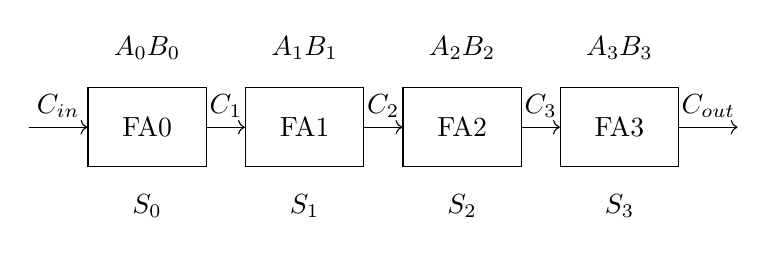
\begin{tikzpicture}
  \node[draw, minimum width=1.5cm, minimum height=1cm] (fa0) at (0,0) {FA0};
  \node[draw, minimum width=1.5cm, minimum height=1cm] (fa1) at (2,0) {FA1};
  \node[draw, minimum width=1.5cm, minimum height=1cm] (fa2) at (4,0) {FA2};
  \node[draw, minimum width=1.5cm, minimum height=1cm] (fa3) at (6,0) {FA3};

  % Carry chain
  \draw[->] (fa0.east) -- node[above] {$C_1$} (fa1.west);
  \draw[->] (fa1.east) -- node[above] {$C_2$} (fa2.west);
  \draw[->] (fa2.east) -- node[above] {$C_3$} (fa3.west);
  \draw[->] (-1.5,0) -- node[above] {$C_{in}$} (fa0.west);
  \draw[->] (fa3.east) -- node[above] {$C_{out}$} (7.5,0);

  % Inputs
  \node at (0,1) {$A_0 B_0$};
  \node at (2,1) {$A_1 B_1$};
  \node at (4,1) {$A_2 B_2$};
  \node at (6,1) {$A_3 B_3$};

  % Outputs
  \node at (0,-1) {$S_0$};
  \node at (2,-1) {$S_1$};
  \node at (4,-1) {$S_2$};
  \node at (6,-1) {$S_3$};
\end{tikzpicture}
\end{center}

\textbf{关键特点}：每个FA的$C_{out}$接到下一个FA的$C_{in}$。进位像水波一样从低位向高位逐级传递。

\textbf{因此得名：Ripple Carry（行波进位/脉动进位）。}

\section{第五步：结构化设计}

4位行波进位加法器 = 4个FA + 进位链：

\begin{itemize}
  \item 每位独立计算本位的 $S_i$ 和 $C_{i+1}$
  \item 进位 $C_i$ 从低位传到高位
  \item 最关键的路径 = 进位链路径（从 $C_{in}$ 到 $C_{out}$ 经过4个FA）
\end{itemize}

\textbf{延迟分析}：
\begin{itemize}
  \item 每个FA的进位延迟 = 2个门延迟（1个AND + 1个OR）
  \item 4位加法器进位延迟 = $4 \times 2 = 8$个门延迟
  \item $S_3$需要等$C_3$稳定后才能计算
\end{itemize}

\section{第六步：为什么这样设计}

\begin{enumerate}
  \item \textbf{为什么进位要逐位传递？}

  因为低位的结果（是否有进位）直接影响高位的计算。这是二进制的内在性质：加法有进位传播。

  \item \textbf{行波进位的优缺点？}

  \textbf{优点}：结构简单、面积小
  \textbf{缺点}：速度慢（进位链延迟随位宽线性增长）

  \item \textbf{为什么还有超前进位加法器（Carry Lookahead）？}

  为突破行波进位速度限制而设计——提前并行计算所有进位，不等待进位传递。但考试通常只考行波进位。
\end{enumerate}

\section{第七步：考试常见变式}

\begin{enumerate}
  \item \textbf{变式1：8位/16位加法器（级联4位加法器）}

  低位加法器的 $C_{out}$ 接到高位加法器的 $C_{in}$。

  \item \textbf{变式2：减法器（用加法器实现减法）}

  $A - B = A + (\sim B + 1)$ = $A + \text{补码}(B)$

  将B取反，$C_{in}=1$，则：$A + (\sim B) + 1 = A - B$。

  \item \textbf{变式3：加法器 + 寄存器 = 累加器}

  每个时钟周期：$ACC \leftarrow ACC + Input$——计数器的基础！

  \item \textbf{变式4：带溢出检测的加法器}

  溢出条件（有符号数）：两个正数相加得负数，或两个负数相加得正数。

  $Overflow = (A_3 \odot B_3) \cdot (A_3 \oplus S_3)$（最高位的符号变化）

  \item \textbf{变式5：BCD加法器}

  二进制加法后如果结果>9，则+6修正。$C_{out} = (S > 9)$ 或 $(C_{out\_binary} = 1)$。
\end{enumerate}

\section{第八步：VHDL实现}

\begin{lstlisting}[caption={4位加法器VHDL实现（行为级）}]
library ieee;
use ieee.std_logic_1164.all;
use ieee.std_logic_unsigned.all;  -- 需要此包以支持算术运算

entity adder_4bit is
  port (
    A    : in  std_logic_vector(3 downto 0);
    B    : in  std_logic_vector(3 downto 0);
    Cin  : in  std_logic;
    Sum  : out std_logic_vector(3 downto 0);
    Cout : out std_logic
  );
end adder_4bit;

architecture behavioral of adder_4bit is
  signal result : std_logic_vector(4 downto 0);
begin
  result <= ('0' & A) + ('0' & B) + Cin;
  Sum  <= result(3 downto 0);
  Cout <= result(4);
end behavioral;
\end{lstlisting}

\begin{lstlisting}[caption={结构级实现（4个全加器级联）}]
architecture structural of adder_4bit is
  signal carry : std_logic_vector(4 downto 0);

  component full_adder is
    port (A, B, Cin : in std_logic; Sum, Cout : out std_logic);
  end component;
begin
  carry(0) <= Cin;

  gen_fa: for i in 0 to 3 generate
    fa_i: full_adder port map (
      A    => A(i),
      B    => B(i),
      Cin  => carry(i),
      Sum  => Sum(i),
      Cout => carry(i+1)
    );
  end generate;

  Cout <= carry(4);
end structural;
\end{lstlisting}

\section{第九步：Testbench验证}

\begin{lstlisting}[caption={4位加法器Testbench}]
library ieee;
use ieee.std_logic_1164.all;
use ieee.std_logic_unsigned.all;

entity adder_4bit_tb is
end adder_4bit_tb;

architecture test of adder_4bit_tb is
  signal A, B, Sum : std_logic_vector(3 downto 0);
  signal Cin, Cout : std_logic;

  component adder_4bit is
    port (
      A    : in  std_logic_vector(3 downto 0);
      B    : in  std_logic_vector(3 downto 0);
      Cin  : in  std_logic;
      Sum  : out std_logic_vector(3 downto 0);
      Cout : out std_logic
    );
  end component;
begin
  uut: adder_4bit port map (A, B, Cin, Sum, Cout);

  stimulus: process
  begin
    Cin <= '0';
    A <= "0011"; B <= "0101"; wait for 10 ns;  -- 3+5=8
    A <= "1010"; B <= "0110"; wait for 10 ns;  -- 10+6=16 -> Cout=1
    A <= "1111"; B <= "0001"; wait for 10 ns;  -- 15+1=16 -> Cout=1
    A <= "0000"; B <= "0000"; wait for 10 ns;  -- 0+0=0
    wait;
  end process;
end test;
\end{lstlisting}

\section{第十步：如何快速解题}

\begin{examtip}[加法器快速解题法]
\begin{enumerate}
  \item \textbf{行为级VHDL}：直接用 \texttt{+} 运算符，最简洁
  \item \textbf{结构级}：generate循环实例化FA，进位链串联
  \item \textbf{减法}：$\sim B + 1 + A$ = $A - B$
  \item \textbf{常考组合}：加法器 + 寄存器 = 累加器（计数器的基础！）
  \item \textbf{溢出判断}：有符号数用$C_{n} \oplus C_{n-1}$，无符号数用$C_{out}$
\end{enumerate}
\end{examtip}

\section{变式详解}
\chapter{4位加法器——5大变式详解}

\section{变式1：8位/16位加法器（级联）}

\begin{detailbox}[完整教学]
\textbf{【方案】}两片4位加法器级联。低位$C_{out}$→高位$C_{in}$。

\textbf{【VHDL——结构级】}
\begin{lstlisting}
add_lo: entity work.adder_4bit port map(A=>A(3 downto 0), B=>B(3 downto 0),
        Cin=>'0', Sum=>Sum(3 downto 0), Cout=>carry);
add_hi: entity work.adder_4bit port map(A=>A(7 downto 4), B=>B(7 downto 4),
        Cin=>carry, Sum=>Sum(7 downto 4), Cout=>Cout);
\end{lstlisting}

\textbf{【行为级——推荐】}
\begin{lstlisting}
signal result : std_logic_vector(8 downto 0);
result <= ('0' & A) + ('0' & B);
Sum <= result(7 downto 0); Cout <= result(8);
\end{lstlisting}
综合器自动优化任意位宽加法。
\end{detailbox}


\section{变式2：减法器（用加法器实现A-B）}

\begin{detailbox}[完整教学]
\textbf{【补码原理】}$A-B = A+(-B) = A+(\sim B+1) = A+\sim B+1$

\textbf{【电路】}B取反→接加法器B输入。$C_{in}=1$（实现+1）。$C_{in}$就是补码中的"+1"。

\textbf{【VHDL】}
\begin{lstlisting}
diff <= A + (not B) + '1';  -- A-B = A + (~B) + 1
-- 或直接用减法运算符
diff <= A - B;
\end{lstlisting}

\begin{examfocus}
\textbf{常考}：为什么$C_{in}=1$能实现减法？
答案：$A-B = A+(\sim B)+1$ → +1部分由$C_{in}=1$提供。
\end{examfocus}
\end{detailbox}


\section{变式3：加法器+寄存器=累加器}

\begin{detailbox}[完整教学]
\textbf{【结构】}加法器计算$ACC+Input$。结果在时钟沿存入ACC。ACC输出反馈回加法器输入端。

\textbf{【VHDL】}
\begin{lstlisting}
process(clk, rst_n)
begin
  if rst_n='0' then acc <= (others=>'0');
  elsif rising_edge(clk) then
    acc <= acc + input_data;  -- 每个时钟累加一次
  end if;
end process;
\end{lstlisting}

\textbf{【本质】}累加器=计数器的一种（不是每次+1，而是+任意值）。

\textbf{【应用】}DSP中的乘累加(MAC)、积分器。
\end{detailbox}


\section{变式4：带溢出检测的加法器}

\begin{detailbox}[完整教学]
\textbf{【无符号数溢出】}$C_{out}=1$=溢出（结果超过最大值）。

\textbf{【有符号数溢出】}$Overflow = C_n \oplus C_{n-1}$（最高位进位和次高位进位异或）。

\textbf{【VHDL】}
\begin{lstlisting}
signal result : std_logic_vector(4 downto 0);  -- 5位
result <= ('0' & A) + ('0' & B);
Sum <= result(3 downto 0);
Cout <= result(4);
-- 有符号溢出
Overflow <= result(4) xor result(3);  -- C4 xor C3
\end{lstlisting}

\textbf{【直观判断】}
两个正数相加得负数 → 溢出 (正溢出)
两个负数相加得正数 → 溢出 (负溢出)
\end{detailbox}


\section{变式5：BCD加法器}

\begin{detailbox}[完整教学]
\textbf{【问题】}二进制加法后，如果结果>9(1001)，需要+6(0110)修正为BCD格式。

\textbf{【VHDL】}
\begin{lstlisting}
signal bin_sum : std_logic_vector(4 downto 0);
signal bcd_sum : std_logic_vector(3 downto 0);
begin
  bin_sum <= ('0' & A) + ('0' & B);
  bcd_sum <= bin_sum(3 downto 0) when bin_sum <= 9
        else bin_sum(3 downto 0) + "0110";  -- >9时+6修正
  Cout <= '1' when bin_sum > 9 else '0';
\end{lstlisting}

\textbf{【例子】}5+7=12(1100)。1100+0110=10010→BCD: 0001 0010(12)。
\end{detailbox}

\chapter{级联二选一数据选择器}

\section{第一步：解决什么问题}

单个2选1 MUX只能从2路数据中选择1路。如果要从更多路数据中选择，怎么办？

\textbf{方案}：用多个2选1 MUX级联，构建更大的MUX。

\begin{keypoint}[级联MUX的本质]
用最基础的2选1 MUX作为构建单元，通过\textbf{分层选择}的方式扩展选择能力。

2选1 $\to$ 4选1 $\to$ 8选1 $\to$ 16选1 $\to$ ...
\end{keypoint}

\section{第二步：用2选1 MUX构建4选1 MUX}

先看2选1 MUX的基本符号：$Y = \overline{S} \cdot D_0 + S \cdot D_1$

\textbf{用3个2选1 MUX构建4选1 MUX}：

\begin{center}
\begin{tikzpicture}
  % First layer: two 2:1 MUXes
  \node[draw, minimum width=2cm, minimum height=0.8cm] (mux0) at (0,2) {MUX 2:1};
  \node[draw, minimum width=2cm, minimum height=0.8cm] (mux1) at (0,0) {MUX 2:1};
  % Second layer: one 2:1 MUX
  \node[draw, minimum width=2cm, minimum height=0.8cm] (mux2) at (4,1) {MUX 2:1};

  % Inputs to first layer
  \node (D0) at (-3,2.5) {$D_0$}; \draw[->] (D0) -- (mux0);
  \node (D1) at (-3,1.5) {$D_1$}; \draw[->] (D1) -- (mux0);
  \node (D2) at (-3,0.5) {$D_2$}; \draw[->] (D2) -- (mux1);
  \node (D3) at (-3,-0.5) {$D_3$}; \draw[->] (D3) -- (mux1);

  % First layer outputs to second layer
  \draw[->] (mux0.east) -- ++(0.5,0) |- (mux2.west |- 2);
  \draw[->] (mux1.east) -- ++(0.5,0) |- (mux2.west |- 0);

  % Selection
  \node (S0) at (-2,-2) {$S_0$};
  \draw[->] (S0) -- (0,-1.5) node[above] {};

  \node (S1) at (4,-2) {$S_1$};

  % Output
  \node (Y) at (7,1) {$Y$};
  \draw[->] (mux2.east) -- (Y);
\end{tikzpicture}
\end{center}

\textbf{工作原理}：
\begin{itemize}
  \item $S_0$ 控制第一层两个MUX：分别从 $(D_0,D_1)$ 和 $(D_2,D_3)$ 中各选一个
  \item $S_1$ 控制第二层MUX：从第一层两个结果中选一个
  \item 结果：$(S_1,S_0)$ 决定了选择 $D_0, D_1, D_2, D_3$ 中的哪一个
\end{itemize}

\section{第三步：真值表}

\begin{center}
\begin{tabular}{|c|c||c|c|c|}
\hline
$S_1$ & $S_0$ & 第一层左MUX输出 & 第一层右MUX输出 & 最终输出 $Y$ \\
\hline
0 & 0 & $D_0$ & $D_2$ & $D_0$ \\
0 & 1 & $D_1$ & $D_3$ & $D_1$ \\
1 & 0 & $D_0$ & $D_2$ & $D_2$ \\
1 & 1 & $D_1$ & $D_3$ & $D_3$ \\
\hline
\end{tabular}
\end{center}

\section{第四步：逻辑推导}

级联MUX的逻辑表达式可以通过代入法推导：

第一层输出：
\begin{align}
  F_0 &= \overline{S_0} \cdot D_0 + S_0 \cdot D_1 \\
  F_1 &= \overline{S_0} \cdot D_2 + S_0 \cdot D_3
\end{align}

第二层输出：
\begin{align}
  Y &= \overline{S_1} \cdot F_0 + S_1 \cdot F_1 \\
    &= \overline{S_1} \cdot (\overline{S_0} \cdot D_0 + S_0 \cdot D_1)
     + S_1 \cdot (\overline{S_0} \cdot D_2 + S_0 \cdot D_3) \\
    &= \overline{S_1}\cdot\overline{S_0}\cdot D_0
     + \overline{S_1}\cdot S_0 \cdot D_1
     + S_1\cdot\overline{S_0} \cdot D_2
     + S_1\cdot S_0 \cdot D_3
\end{align}

\textbf{这正是标准4选1 MUX的逻辑表达式！} 证明级联等价于一个完整的$2^n$选1 MUX。

\section{第五步：结构化设计——通用级联规律}

\textbf{树形结构}：

\begin{itemize}
  \item \textbf{第一层}：$2^{n-1}$ 个2选1 MUX（用最低位 $S_0$ 选择）
  \item \textbf{第二层}：$2^{n-2}$ 个2选1 MUX（用 $S_1$ 选择）
  \item \textbf{...}
  \item \textbf{第n层}：1个2选1 MUX（用最高位 $S_{n-1}$ 选择）
\end{itemize}

总MUX数量：$2^n - 1$ 个2选1 MUX。

\section{第六步：为什么这样设计}

\begin{enumerate}
  \item \textbf{为什么2选1是基础构建块？}

  2选1 MUX是最简单的MUX（1位选择线），在FPGA中通常对应一个LUT（查找表）。任何更大的MUX都可以由2选1 MUX级联构建。

  \item \textbf{树形结构的深层意义？}

  每一层将数据组数减半：
  \begin{itemize}
    \item 输入：$2^n$ 路数据
    \item 第一层后：$2^{n-1}$ 路
    \item 第二层后：$2^{n-2}$ 路
    \item ...
    \item 第n层后：1路（最终输出）
  \end{itemize}

  这本质上是锦标赛淘汰赛的结构——每一轮淘汰一半。

  \item \textbf{延迟分析}：

  级联MUX的关键路径（从数据输入到输出）经过 $n$ 级2选1 MUX。每级延迟约1-2个门延迟。
\end{enumerate}

\section{第七步：考试常见变式}

\begin{enumerate}
  \item \textbf{变式1：用2选1 MUX构建8选1 MUX}

  需要 $2^3 - 1 = 7$ 个2选1 MUX。三层结构：4+2+1。

  \item \textbf{变式2：用4选1 MUX构建16选1 MUX}

  5片4选1 MUX：4片第一层 + 1片第二层（作为最终选择）。

  \item \textbf{变式3：不对称级联}

  例如：用1片4选1 + 1片2选1构建6选1 MUX（实际数据输入不足$2^n$个时的处理方法）。

  \item \textbf{变式4：MUX树实现逻辑函数}

  将逻辑函数的变量从低位到高位接选择线，用MUX树实现多变量函数。这是MUX做通用逻辑的关键应用。
\end{enumerate}

\section{第八步：VHDL实现}

\begin{lstlisting}[caption={用2选1 MUX级联构建4选1 MUX（结构级）}]
library ieee;
use ieee.std_logic_1164.all;

entity mux2to1 is
  port (
    D0, D1 : in  std_logic;
    S      : in  std_logic;
    Y      : out std_logic
  );
end mux2to1;

architecture behavioral of mux2to1 is
begin
  Y <= D0 when S = '0' else D1;
end behavioral;

-- ========================================

library ieee;
use ieee.std_logic_1164.all;

entity mux4to1_cascade is
  port (
    D : in  std_logic_vector(3 downto 0);
    S : in  std_logic_vector(1 downto 0);
    Y : out std_logic
  );
end mux4to1_cascade;

architecture structural of mux4to1_cascade is
  signal F0, F1 : std_logic;  -- 第一层输出

  component mux2to1 is
    port (D0, D1 : in std_logic; S : in std_logic; Y : out std_logic);
  end component;
begin
  -- 第一层：S(0)选择
  mux_a: mux2to1 port map (D(0), D(1), S(0), F0);
  mux_b: mux2to1 port map (D(2), D(3), S(0), F1);
  -- 第二层：S(1)选择
  mux_c: mux2to1 port map (F0, F1, S(1), Y);
end structural;
\end{lstlisting}

\section{第九步：Testbench验证}

\begin{lstlisting}[caption={级联MUX Testbench}]
library ieee;
use ieee.std_logic_1164.all;

entity mux4to1_cascade_tb is
end mux4to1_cascade_tb;

architecture test of mux4to1_cascade_tb is
  signal D : std_logic_vector(3 downto 0);
  signal S : std_logic_vector(1 downto 0);
  signal Y : std_logic;

  component mux4to1_cascade is
    port (
      D : in  std_logic_vector(3 downto 0);
      S : in  std_logic_vector(1 downto 0);
      Y : out std_logic
    );
  end component;
begin
  uut: mux4to1_cascade port map (D, S, Y);

  stimulus: process
  begin
    D <= "1010";
    S <= "00"; wait for 10 ns;  -- Y=D0=0
    S <= "01"; wait for 10 ns;  -- Y=D1=1
    S <= "10"; wait for 10 ns;  -- Y=D2=0
    S <= "11"; wait for 10 ns;  -- Y=D3=1
    wait;
  end process;
end test;
\end{lstlisting}

\section{第十步：如何快速解题}

\begin{examtip}[级联MUX快速解题法]
\begin{enumerate}
  \item \textbf{$n$选1 MUX所需2选1 MUX数目} = $n-1$
  \item \textbf{树形结构}：每层将数据组数减半
  \item \textbf{选择位分配}：最低位控制第一层，最高位控制最后一层
  \item \textbf{关键路径} = $n$级2选1 MUX延迟（$n = \log_2(N)$）
\end{enumerate}
\end{examtip}

\textbf{秒杀：用2选1 MUX构建任意MUX的公式}

$2^n$选1 MUX 需要 $(2^n - 1)$ 个2选1 MUX，分 $n$ 层。第 $k$ 层（从1开始）有 $2^{n-k}$ 个MUX，由 $S_{k-1}$ 控制。

\section{变式详解}
\chapter{级联MUX——4大变式详解}

\section{变式1：用2选1 MUX构建8选1 MUX}

\begin{detailbox}[完整教学]
\textbf{【树形结构】}3层：第一层4个→第二层2个→第三层1个=7个2选1 MUX。

\textbf{【选择位分配】}
\begin{itemize}
  \item S0→第一层(4个MUX)：每两组数据中选一个
  \item S1→第二层(2个MUX)：第一层结果中两两选择
  \item S2→第三层(1个MUX)：第二层两个结果中最终选择
\end{itemize}

\textbf{【通用公式】}$2^n$选1 MUX需要$2^n-1$个2选1 MUX，分$n$层。

\textbf{【VHDL——generate结构级】}
\begin{lstlisting}[caption={8选1 MUX（2选1树形级联）}]
library ieee;
use ieee.std_logic_1164.all;

entity mux8to1_cascade is
  port (
    D : in  std_logic_vector(7 downto 0);
    S : in  std_logic_vector(2 downto 0);
    Y : out std_logic
  );
end mux8to1_cascade;

architecture behavioral of mux8to1_cascade is
  -- 递归描述流水线MUX树
  signal layer0 : std_logic_vector(3 downto 0);
  signal layer1 : std_logic_vector(1 downto 0);
begin
  gen0: for i in 0 to 3 generate
    layer0(i) <= D(2*i) when S(0)='0' else D(2*i+1);
  end generate;
  gen1: for i in 0 to 1 generate
    layer1(i) <= layer0(2*i) when S(1)='0' else layer0(2*i+1);
  end generate;
  Y <= layer1(0) when S(2)='0' else layer1(1);
end behavioral;
\end{lstlisting}
\end{detailbox}


\section{变式2：用4选1 MUX构建16选1 MUX}

\begin{detailbox}[完整教学]
\textbf{【结构】}第一层4片4选1 MUX，第二层1片4选1 MUX。共5片。

S1S0→第一层(4片4选1 MUX)。S3S2→第二层(1片4选1 MUX选择第一层输出之一)。
\end{detailbox}


\section{变式3：不对称级联（构建6选1 MUX）}

\begin{detailbox}[完整教学]
\textbf{【问题】}需要6选1，但MUX只有$2^n$选1。用8选1实现6选1（两个输入悬空或接地）。

\textbf{【VHDL——4选1+2选1】}
\begin{lstlisting}[caption={6选1 MUX（4选1+2选1级联）}]
library ieee;
use ieee.std_logic_1164.all;

entity mux6to1_asymmetric is
  port (
    D : in  std_logic_vector(5 downto 0);
    S : in  std_logic_vector(2 downto 0);
    Y : out std_logic
  );
end mux6to1_asymmetric;

architecture structural of mux6to1_asymmetric is
  signal mux4_out : std_logic;

  component mux4to1 is
    port (
      D : in  std_logic_vector(3 downto 0);
      S : in  std_logic_vector(1 downto 0);
      Y : out std_logic
    );
  end component;
begin
  -- 第一层：4选1处理D0-D3
  mux4: mux4to1 port map(D=>D(3 downto 0), S=>S(1 downto 0), Y=>mux4_out);
  -- 顶层：2选1在mux4_out和D4/D5间选择
  Y <= mux4_out when S(2)='0' else
       D(4) when S(1 downto 0)="00" else D(5);
  -- 注意：S2=1时S1S0只需表示2种状态即可
end structural;
\end{lstlisting}

\textbf{【简化方案】}直接用8选1 MUX，D6和D7接地(固定为0)。
\end{detailbox}


\section{变式4：MUX树实现逻辑函数}

\begin{detailbox}[完整教学]
\textbf{【本质】}MUX=通用逻辑实现器。MUX树=多层选择=分而治之。

\textbf{【Shannon展开定理】}$F(x_1,x_2,\dots,x_n)= \overline{x_1}\cdot F(0,x_2,\dots,x_n) + x_1\cdot F(1,x_2,\dots,x_n)$

这正是2选1 MUX的表达式！递归应用=构建MUX树。

\textbf{【结论】}任何组合逻辑函数都可用2选1 MUX树实现——这其实就是FPGA中LUT的工作原理。
\end{detailbox}

\chapter{组合逻辑电路：统一设计套路}

\section{什么是组合逻辑电路}

回顾我们学过的7个电路，它们有一个共同特征：

\begin{keypoint}[组合逻辑电路的定义]
\textbf{输出仅由当前输入决定，与历史状态无关。}

没有记忆、没有反馈、没有时钟。

给定输入 → 直接得到输出（经过一定的门延迟）。
\end{keypoint}

\section{组合逻辑电路谱系}

所有组合逻辑电路可以分为三类：

\begin{enumerate}
  \item \textbf{编码/译码类}

  \begin{itemize}
    \item 编码器（8-3）：$2^n \to n$ 压缩，OR逻辑
    \item 译码器（3-8）：$n \to 2^n$ 展开，AND逻辑（最小项）
    \item BCD译码器：4位BCD $\to$ 7段显示
  \end{itemize}

  编码器和译码器是\textbf{互为逆过程}。

  \item \textbf{数据通路类}

  \begin{itemize}
    \item MUX（4选1）：选择数据来源
    \item 级联MUX：从小MUX构建大MUX
  \end{itemize}

  MUX是组合逻辑的"万能积木"——任何组合逻辑函数都可以用MUX实现。

  \item \textbf{运算类}

  \begin{itemize}
    \item 比较器：判断 $A>B, A=B, A<B$，从高位到低位优先级
    \item 加法器：$A+B+C_{in}$，进位链串联
  \end{itemize}
\end{enumerate}

\section{统一设计套路}

当你面对一个需要设计组合逻辑电路的考试题时，按以下步骤：

\begin{designflow}[组合逻辑电路统一设计流程]
\begin{enumerate}
  \item \textbf{明确输入输出}：几个输入？几位？几个输出？每位含义？
  \item \textbf{列真值表}：穷举所有输入组合，写出对应输出
  \item \textbf{推导逻辑表达式}：从真值表提取每个输出位的逻辑函数
  \item \textbf{选择实现方式}：
  \begin{itemize}
    \item 门级实现：手写与或表达式
    \item MUX实现：真值表输出列接到MUX数据输入端
    \item 译码器+OR实现：最小项之和
    \item VHDL实现：case / with-select / if-else（推荐！）
  \end{itemize}
  \item \textbf{写VHDL}：case覆盖所有情况，when others兜底
  \item \textbf{验证}：检查边界条件
\end{enumerate}
\end{designflow}

\section{考试中最高频的组合逻辑考点}

\begin{enumerate}
  \item \textbf{用MUX实现任意逻辑函数}（必考）

  $2^n$选1 MUX实现$n$变量函数：选择线接变量，数据输入接函数值

  \item \textbf{用译码器+OR门实现任意逻辑函数}（必考）

  译码器产生所有最小项，OR门选择需要的项

  \item \textbf{优先级编码器的VHDL实现}（常考）

  if-else级联：优先级从高到低

  \item \textbf{74LS138使能端级联扩展}（常考）

  高位地址做片选，低位地址接输入

  \item \textbf{加法器+寄存器=累加器}（承上启下）

  这是从组合逻辑过渡到时序逻辑的关键桥梁
\end{enumerate}

\section{从组合逻辑到时序逻辑}

到目前为止，所有电路都有一个根本限制：

\begin{center}
\fbox{%
\begin{minipage}{0.85\textwidth}
\textbf{组合逻辑不能存储信息。}

电路的输出只取决于当前输入。当输入消失或改变，旧的结果就丢失了。

\vspace{0.3cm}
这不是设计缺陷——这是组合逻辑的本质。

\vspace{0.3cm}
如果我们需要"记住"一个值，需要存储"当前状态"，那就必须引入\textbf{时序逻辑}。
\end{minipage}%
}
\end{center}

而这个过渡的桥梁就是——\textbf{D触发器}。

组合逻辑 + 存储单元（D触发器） = 时序逻辑 = 状态机

\textbf{这将在第二部分详细展开。}


% =============================================================
%  第二部分：D触发器体系
% =============================================================
\part{D触发器体系}

\chapter{D触发器深度解析}

\section{为什么组合逻辑不能存储信息}

让我们做一个思维实验。

假设你想"记住"数字5。你用一个组合逻辑电路产生输出5：

\begin{center}
\begin{tikzpicture}
  \node[draw, minimum width=3cm, minimum height=1.5cm] (cl) at (0,0) {组合逻辑};
  \node (in) at (-3,0) {输入(某种编码)};
  \node (out) at (3,0) {输出 = 5};
  \draw[->] (in) -- (cl);
  \draw[->] (cl) -- (out);
\end{tikzpicture}
\end{center}

\textbf{问题来了}：如果切断输入（或输入改变），5就消失了。

组合逻辑的输出\textbf{始终等于}$f(\text{输入})$。没有输入就没有输出。输出不能独立于输入而存在。

\begin{keypoint}[组合逻辑的根本限制]
组合逻辑 = 无记忆电路

输出$(t) = f($输入$(t))$——输出在任何时刻都直接由当前输入决定。

它不能脱离输入而独立"保持"一个值。
\end{keypoint}

\section{为什么需要存储}

数字系统中大量的操作需要"记住"值：

\begin{itemize}
  \item 计数器需要记住"当前计到几了"
  \item 寄存器需要记住"上次存了哪个数"
  \item 状态机需要记住"我当前在哪个状态"
  \item 累加器需要记住"累加和是多少"
\end{itemize}

这些都是"信息需要跨越时间而保持"的场景。

\textbf{跨越时间} = 记忆 = 存储 = 需要一种能"保持"信息的元件。

\section{什么叫状态？什么叫记忆？}

\begin{definition}[状态]
\textbf{状态} = 系统在某个时刻的全部内部信息的快照。

时钟驱动下，状态的变迁构成了时序电路的行为。
\end{definition}

\begin{definition}[记忆]
\textbf{记忆} = 在输入消失后，信息仍然被保留的能力。

D触发器的记忆：在时钟上升沿捕获D输入，之后即使D改变，Q输出保持上一次捕获的值不变，直到下一个时钟上升沿。
\end{definition}

\section{D触发器到底保存了什么}

\begin{keypoint}[D触发器的本质]
\textbf{D触发器是一个1-bit存储单元。}

\begin{itemize}
  \item 它在每个时钟上升沿"采样"D输入的值
  \item 将采样到的值保持到输出Q上
  \item 这个值一直保持到下一个时钟上升沿
\end{itemize}
\end{keypoint}

\subsection{D触发器的输入输出}

\begin{itemize}
  \item \textbf{D（Data）}：数据输入——下一个时钟沿要存储什么值
  \item \textbf{CLK（Clock）}：时钟信号——决定"什么时候"采样
  \item \textbf{Q}：数据输出——当前存储的值
  \item \textbf{$\overline{Q}$}：Q的反相（部分D触发器有此输出）
\end{itemize}

\section{时钟上升沿发生什么}

当时钟从0变1的那一瞬间（上升沿$\uparrow$），D触发器做一件事：

\begin{center}
\fbox{%
\begin{minipage}{0.8\textwidth}
\begin{center}
\textbf{采样D的值} $\to$ \textbf{锁存到内部} $\to$ \textbf{驱动到Q输出}
\end{center}
\end{minipage}%
}
\end{center}

\textbf{在上升沿之前}：Q保持旧值（上一次采样时的D值）

\textbf{在上升沿那一瞬间}：Q更新为新值（当前D的值）

\textbf{在上升沿之后}：即使D变化，Q保持不变（直到下一个上升沿）

\subsection{逐拍分析：D触发器的一次工作过程}

假设初始状态：Q = 0。

\begin{beatanalysis}[D触发器单次采样过程]
\begin{center}
\begin{tabular}{|c|c|c|c|}
\hline
\textbf{时刻} & \textbf{CLK} & \textbf{D} & \textbf{Q} \\
\hline
上升沿到达前 & 0 & 1 & 0 （保持旧值）\\
\textbf{上升沿瞬间} & 0→1（$\uparrow$）& 1 & \textbf{1}（采样并更新！）\\
上升沿之后 & 1 & 0 & 1 （保持采样值，不理D变化）\\
上升沿之后 & 1 & x（任意）& 1 （仍然保持）\\
下一次上升沿 & 0→1（$\uparrow$）& 0 & \textbf{0}（采样新的D值！）\\
\hline
\end{tabular}
\end{center}
\end{beatanalysis}

\textbf{关键洞察}：
\begin{itemize}
  \item 在非上升沿时刻，D可以随便变化，Q纹丝不动
  \item 只有上升沿那一瞬间，D的值被"捕获"
  \item 捕获后Q保持该值，像一个"时间冻结"的样本
\end{itemize}

\section{Q(n)和Q(n+1)到底是什么意思}

这是数字逻辑中最核心的概念之一：

\begin{definition}[Q(n) vs Q(n+1)]
\begin{itemize}
  \item \textbf{Q(n)} = 第n个时钟周期内（上升沿之后），触发器的\textbf{当前}输出
  \item \textbf{Q(n+1)} = 第n+1个时钟上升沿到达后，触发器的\textbf{下一个}输出
\end{itemize}

Q(n) 和 Q(n+1) 之间恰好差一个时钟周期。
\end{definition}

对于D触发器：

\begin{equation}
  \boxed{Q(n+1) = D(n)}
\end{equation}

\textbf{含义}：下一个时钟上升沿之后Q的值 = 当前上升沿时采样的D值。

\begin{center}
\begin{tikzpicture}
  \draw[->] (0,0) -- (8,0) node[right] {时间};
  \draw (1,0.5) -- (1,-0.5) node[below] {第n拍};
  \draw (3,0.5) -- (3,-0.5);
  \draw (5,0.5) -- (5,-0.5) node[below] {第n+1拍};
  \draw (7,0.5) -- (7,-0.5) node[below] {第n+2拍};

  \node at (1,0.8) {$\uparrow$};
  \node at (3,0.8) {$\uparrow$};
  \node at (5,0.8) {$\uparrow$};
  \node at (7,0.8) {$\uparrow$};

  \node at (2,1.5) {Q保持D(上一拍值)};
  \node at (4,1.5) {Q(n)};
  \node at (6,1.5) {Q(n+1)=D(n)};
\end{tikzpicture}
\end{center}

\section{FPGA中的寄存器资源与D触发器关系}

\begin{keypoint}[FPGA寄存器的本质]
FPGA中的"寄存器"(Register/Flip-Flop)就是一个D触发器。

\begin{itemize}
  \item 每个LE（Logic Element）/Slice包含若干个D触发器
  \item 当你在VHDL中写 \texttt{signal x : std\_logic} 并在process中赋值，综合器就把x映射到一个D触发器
  \item \texttt{std\_logic\_vector(7 downto 0)} = 8个D触发器并排
\end{itemize}
\end{keypoint}

总结关系：

\begin{center}
\begin{tikzpicture}
  \node[draw, minimum width=2.5cm, minimum height=1cm] (vhdl) at (0,2) {VHDL signal};
  \node[draw, minimum width=2.5cm, minimum height=1cm] (dff) at (0,0) {D触发器};
  \node[draw, minimum width=2.5cm, minimum height=1cm] (fpga) at (0,-2) {FPGA寄存器};

  \draw[->] (vhdl) -- (dff) node[midway,right] {综合成};
  \draw[->] (dff) -- (fpga) node[midway,right] {对应};

  \node[draw, minimum width=2.5cm, minimum height=1cm] (vec) at (5,2) {vector(7:0)};
  \node[draw, minimum width=2.5cm, minimum height=1cm] (8dff) at (5,0) {8个D触发器};
  \node[draw, minimum width=2.5cm, minimum height=1cm] (8reg) at (5,-2) {8个寄存器};

  \draw[->] (vec) -- (8dff) node[midway,right] {综合成};
  \draw[->] (8dff) -- (8reg) node[midway,right] {对应};
\end{tikzpicture}
\end{center}

\section{D触发器的VHDL实现}

\begin{lstlisting}[caption={D触发器VHDL实现（带异步复位）}]
library ieee;
use ieee.std_logic_1164.all;

entity dff is
  port (
    clk   : in  std_logic;
    rst_n : in  std_logic;  -- 异步复位（低有效）
    D     : in  std_logic;
    Q     : out std_logic
  );
end dff;

architecture behavioral of dff is
begin
  process(clk, rst_n)
  begin
    if rst_n = '0' then
      Q <= '0';              -- 异步复位
    elsif rising_edge(clk) then
      Q <= D;                -- 时钟上升沿：采样D并输出到Q
    end if;
  end process;
end behavioral;
\end{lstlisting}

\subsection{VHDL中的关键点}

\begin{enumerate}
  \item \texttt{process(clk, rst\_n)}：敏感信号列表包含CLK和复位
  \item \texttt{if rst\_n = '0' then}：异步复位优先——复位不受时钟控制
  \item \texttt{elsif rising\_edge(clk) then}：这才是"边沿触发"——只有在上升沿才执行
  \item \texttt{Q <= D}：这是D触发器的核心行为——$Q(n+1) = D(n)$
\end{enumerate}

\subsection{综合成什么硬件}

\begin{center}
\begin{tikzpicture}
  % D Flip-Flop schematic
  \node[draw, minimum width=2cm, minimum height=3cm, label=above:D触发器] (dff) at (0,0) {};
  \node (D) at (-2,1) {D};
  \node (clk) at (-2,0) {CLK};
  \node (rst) at (-2,-1) {rst\_n};
  \node (Q) at (2,0) {Q};

  \draw[->] (D) -- (dff.west |- D);
  \draw[->] (clk) -- (dff.west |- clk);
  \draw[->] (rst) -- (dff.west |- rst);
  \draw[->] (dff.east |- Q) -- (Q);

  \node at (0,-2.5) {\small 内部：主从锁存器结构};
\end{tikzpicture}
\end{center}

\section{D触发器 + 组合逻辑 = 一切时序电路}

现在我们有：
\begin{itemize}
  \item \textbf{组合逻辑}：能做计算，但不能存储
  \item \textbf{D触发器}：能存储1 bit，但不能计算
\end{itemize}

把它们结合起来：

\begin{center}
\begin{tikzpicture}
  \node[draw, minimum width=2cm, minimum height=1cm] (cl) at (0,2) {组合逻辑};
  \node[draw, minimum width=2cm, minimum height=1cm] (dff) at (0,0) {D触发器};

  \draw[->] (cl.east) -- ++(1,0) |- (dff.east) node[midway,right] {D};
  \draw[->] (dff.west) -- ++(-1,0) |- (cl.west) node[midway,left] {Q（反馈）};

  \node at (3,-2) {\textbf{这就构成了状态机！}};
\end{tikzpicture}
\end{center}

\textbf{Q（状态输出）} $\to$ 组合逻辑计算 $\to$ 产生新的D $\to$ 下一个时钟沿存入D触发器 $\to$ 新状态！

这就是所有同步时序电路的核心结构。

\begin{keypoint}[时序电路核心模型]
$$\text{当前状态} \xrightarrow{\text{组合逻辑}} \text{下一状态} \xrightarrow{\text{时钟沿}} \text{存入D触发器}$$

时钟驱动状态向前流动。每个时钟周期，状态更新一次。
\end{keypoint}

\section{Testbench验证}

\begin{lstlisting}[caption={D触发器Testbench}]
library ieee;
use ieee.std_logic_1164.all;

entity dff_tb is
end dff_tb;

architecture test of dff_tb is
  signal clk, rst_n, D, Q : std_logic;
  constant clk_period : time := 20 ns;

  component dff is
    port (clk, rst_n, D : in std_logic; Q : out std_logic);
  end component;
begin
  uut: dff port map (clk, rst_n, D, Q);

  -- 时钟生成
  clk_process: process
  begin
    clk <= '0'; wait for clk_period/2;
    clk <= '1'; wait for clk_period/2;
  end process;

  -- 测试序列
  stimulus: process
  begin
    rst_n <= '0'; D <= '0'; wait for 30 ns;  -- 复位
    rst_n <= '1';             wait for 5 ns;

    D <= '1'; wait for clk_period;  -- 上升沿采样D=1
    D <= '0'; wait for clk_period;  -- 上升沿采样D=0
    D <= '1'; D <= '0' after 5 ns;  -- 在非上升沿改变D（Q不会变）
    wait for clk_period;
    wait;
  end process;
end test;
\end{lstlisting}

\section{D触发器体系总结}

\begin{enumerate}
  \item \textbf{一个D触发器 = 1 bit存储}：能记住一个二进制位
  \item \textbf{时钟沿触发}：只有在上升沿（或下降沿）才采样和更新
  \item \textbf{Q(n+1) = D(n)}：D触发器的特征方程，一切推导的基础
  \item \textbf{N个D触发器并排}：可以存储N位数据（寄存器）
  \item \textbf{组合逻辑+D触发器}：构成一切同步时序电路
\end{enumerate}

\textbf{下一步}：将D触发器串联起来——得到计数器、移位寄存器、状态机等一切有趣的电路。


% =============================================================
%  第三部分：计数器体系
% =============================================================
\part{计数器体系}

\chapter{计数器统一框架：从状态机视角理解计数器}

\section{最重要的一句话}

\begin{keypoint}[计数器的本质]
\textbf{计数器就是一个状态机，它的状态转移函数是：}

$$\text{下一状态} = \text{当前状态} + 1 \quad (\text{模} N)$$

计数器不是"一个能计数的东西"，而是"一个状态在0到N-1之间循环的时序电路"。
\end{keypoint}

\section{什么是状态}

回顾D触发器：每个D触发器保存1 bit信息。

4个D触发器并排：
\begin{center}
\begin{tikzpicture}
  \node[draw, minimum width=1cm, minimum height=0.8cm] (q3) at (3,0) {Q3};
  \node[draw, minimum width=1cm, minimum height=0.8cm] (q2) at (1.5,0) {Q2};
  \node[draw, minimum width=1cm, minimum height=0.8cm] (q1) at (0,0) {Q1};
  \node[draw, minimum width=1cm, minimum height=0.8cm] (q0) at (-1.5,0) {Q0};

  \node at (3,-1.5) {$\times 8$};
  \node at (1.5,-1.5) {$\times 4$};
  \node at (0,-1.5) {$\times 2$};
  \node at (-1.5,-1.5) {$\times 1$};

  \node at (0.75,-2.5) {存储的值 = $8\times Q_3 + 4\times Q_2 + 2\times Q_1 + 1\times Q_0$};
\end{tikzpicture}
\end{center}

\textbf{状态} = 这四个Q值在某个时刻的\textbf{具体组合}。

例如：
\begin{itemize}
  \item 状态"5" = Q3Q2Q1Q0 = 0101
  \item 状态"12" = Q3Q2Q1Q0 = 1100
  \item 状态"0" = Q3Q2Q1Q0 = 0000
\end{itemize}

\section{什么是状态转移}

\textbf{状态转移}：在时钟沿驱动下，系统从当前状态变为下一个状态。

计数器中的状态转移规则只有一条：

\begin{center}
\fbox{%
\begin{minipage}{0.7\textwidth}
\begin{center}
$$\text{如果当前状态} = i \quad (i < N-1)$$
$$\text{则下一状态} = i + 1$$

$$\text{如果当前状态} = N-1$$
$$\text{则下一状态} = 0$$
\end{center}
\end{minipage}%
}
\end{center}

\textbf{N = 模值——计数器在0 到 N-1之间循环。}

\section{为什么计数器本质是状态机}

状态机有三个要素：
\begin{enumerate}
  \item \textbf{当前状态}：计数器当前计数值
  \item \textbf{状态转移函数}：$S_{next} = (S_{current} + 1) \bmod N$
  \item \textbf{时钟驱动}：每个时钟上升沿，状态更新一次
\end{enumerate}

计数器完美符合状态机的定义。

\begin{center}
\begin{tikzpicture}[scale=0.9, ->, >=stealth, node distance=1.5cm]
  \node[draw, circle] (s0) at (0,0) {0};
  \node[draw, circle] (s1) at (2,0) {1};
  \node[draw, circle] (s2) at (4,0) {2};
  \node[draw, circle] (s3) at (6,0) {3};
  \node[draw, circle] (s4) at (7,2) {...};
  \node[draw, circle] (sn) at (6,4) {N-1};

  \draw (s0) -- (s1);
  \draw (s1) -- (s2);
  \draw (s2) -- (s3);
  \draw (s3) -- (s4);
  \draw (s4) -- (sn);
  \draw (sn) edge[bend right=40] (s0);

  \node at (3,-1.5) {\small 状态循环：0→1→2→3→...→N-1→0→1→...};
\end{tikzpicture}
\end{center}

\section{为什么计数器本质是"当前状态+1"}

这听起来像废话——但这恰恰是最重要的理解。

计数器的核心操作是：

\begin{equation}
  \text{Reg}[3:0] \leftarrow \text{Reg}[3:0] + 1
\end{equation}

用硬件实现：
\begin{enumerate}
  \item \textbf{寄存器}（D触发器组）存储当前计数值（当前状态）
  \item \textbf{加法器}（组合逻辑）计算 "当前状态 + 1"（下一状态）
  \item \textbf{时钟沿}到来时，加法器的输出存入寄存器（状态更新）
\end{enumerate}

\begin{center}
\begin{tikzpicture}
  \node[draw, minimum width=2.5cm, minimum height=1.2cm] (reg) at (0,0) {寄存器（状态）};
  \node[draw, minimum width=2cm, minimum height=1cm] (add) at (4,0) {+1};

  \draw[->] (reg.east) -- (add.west) node[midway,above] {当前状态};
  \draw[->] (add.east) -- ++(1,0) |- (reg.north) node[near end,right] {下一状态};

  \node at (0,-1.5) {\small 反馈环：状态 $\to$ +1 $\to$ 下一状态 $\to$ 存回寄存器};
\end{tikzpicture}
\end{center}

\textbf{这个反馈环是计数器（以及所有状态机）的硬件本质。}

\section{通用计数器设计流程}

\begin{designflow}[通用计数器设计流程——适用于任何模值]
\begin{enumerate}
  \item \textbf{确定模值N}：计数器从0计到N-1，共N个状态
  \item \textbf{确定寄存器位宽k}：$k = \lceil \log_2 N \rceil$（能满足表示N-1的最小位数）
  \item \textbf{设计状态转移}：当前状态 + 1（这是所有二进制计数器的共同逻辑）
  \item \textbf{设计回零条件}：当当前状态 = N-1 时（这是不同计数器的唯一区别）
    \begin{itemize}
      \item 进位置1（表示一轮计数完成）
      \item 下一状态 = 0
    \end{itemize}
  \item \textbf{验证状态完整性}：确保从0到N-1的每个状态都能正确转移，且状态N不会出现
  \item \textbf{转换成VHDL}：
    \begin{itemize}
      \item 标准写法：if rising\_edge(clk) then count <= count + 1;
      \item 加上清零条件：if count = N-1 then count <= 0;
    \end{itemize}
  \end{enumerate}
\end{designflow}

\section{为什么所有计数器本质上是一个问题}

看下面几个需求：
\begin{itemize}
  \item "设计一个模12计数器"：0→1→...→11→0→1→...
  \item "设计一个模24计数器"：0→1→...→23→0→1→...
  \item "设计一个模60计数器"：0→1→...→59→0→1→...
\end{itemize}

它们的\textbf{区别只有一个}：清零条件不同。

\begin{itemize}
  \item 模12：count = 11 时清零（即 1100 时回零）
  \item 模24：count = 23 时清零（即 10111 时回零）
  \item 模60：count = 59 时清零（即 111011 时回零）
\end{itemize}

\textbf{除此之外，其余所有逻辑完全相同！}

这就是为什么我们要建立一个统一框架来理解所有计数器。

\begin{keypoint}[计数器统一公式]
\textbf{任意模N二进制计数器：}

\begin{lstlisting}
 if rising_edge(clk) then
  if count = N-1 then
    count <= 0;
  else
    count <= count + 1;
  end if;
end if;
\end{lstlisting}

唯一的参数：N（模值）
\end{keypoint}

\section{接下来的学习顺序}

在建立了统一框架之后，我们将用这个框架统一推导：

\begin{itemize}
  \item \textbf{4位计数器}（模16，$N = 2^4$）——最基础
  \item \textbf{模12计数器}——$N = 12$，需要4位 + 回零逻辑
  \item \textbf{模24计数器}——$N = 24$，需要5位 + 回零逻辑
  \item \textbf{模60计数器}——$N = 60$，需要6位 + 回零逻辑
  \item \textbf{模为任意值的计数器}——通用设计方法
  \item \textbf{BCD计数器}（模10，B个位/十位分开编码）
  \item \textbf{BCD模24/模60}——多位BCD级联
\end{itemize}

你会发现它们都是从同一个模板稍加修改得到的。

\chapter{4位加法计数器——模$2^N$二进制计数器}

\section{应用统一框架}

\begin{enumerate}
  \item \textbf{模值N}：$N = 2^4 = 16$（4位二进制能表示0到15）
  \item \textbf{寄存器位宽k}：$k = 4$（Q3 Q2 Q1 Q0）
  \item \textbf{状态转移}：count $\leftarrow$ count + 1
  \item \textbf{回零条件}：当 count = 1111（15）时，下一状态自动归0
    \begin{itemize}
      \item 注意：4位二进制1111 + 1 = 10000（5位），但寄存器只有4位，最高位（进位）自然丢弃
      \item 所以\textbf{不需要显式清零}——自然溢出就是模16
    \end{itemize}
\end{enumerate}

\section{逐拍状态分析}

这是全书第一个需要逐拍分析的电路。请仔细看每个时钟周期内发生了什么。

\subsection{初始状态}

\clktick{0}（初始）：
\begin{itemize}
  \item Q3Q2Q1Q0 = 0000（状态0）
  \item 加法器计算：0000 + 1 = 0001
  \item D3D2D1D0 = 0001（准备好下一状态）
\end{itemize}

\subsection{时钟第1拍到第16拍}

\begin{beatanalysis}[4位计数器完整16拍]
\begin{center}
\begin{tabular}{|c|c|c|c|c|c|}
\hline
\textbf{时钟拍} & \textbf{上升沿前Q值} & \textbf{加法器输出}(Q+1) & \textbf{上升沿后Q值} & \textbf{十进制} & \textbf{进位} \\
\hline
1 & 0000 & 0001 & \textbf{0001} & 1 & 0 \\
2 & 0001 & 0010 & \textbf{0010} & 2 & 0 \\
3 & 0010 & 0011 & \textbf{0011} & 3 & 0 \\
4 & 0011 & 0100 & \textbf{0100} & 4 & 0 \\
5 & 0100 & 0101 & \textbf{0101} & 5 & 0 \\
6 & 0101 & 0110 & \textbf{0110} & 6 & 0 \\
7 & 0110 & 0111 & \textbf{0111} & 7 & 0 \\
8 & 0111 & 1000 & \textbf{1000} & 8 & 0 \\
9 & 1000 & 1001 & \textbf{1001} & 9 & 0 \\
10 & 1001 & 1010 & \textbf{1010} & 10 & 0 \\
11 & 1010 & 1011 & \textbf{1011} & 11 & 0 \\
12 & 1011 & 1100 & \textbf{1100} & 12 & 0 \\
13 & 1100 & 1101 & \textbf{1101} & 13 & 0 \\
14 & 1101 & 1110 & \textbf{1110} & 14 & 0 \\
15 & 1110 & 1111 & \textbf{1111} & 15 & 0 \\
16 & 1111 & 0000 & \textbf{0000} & 0 & \textbf{1} \\
\hline
\end{tabular}
\end{center}
\end{beatanalysis}

\textbf{关键观察}：
\begin{itemize}
  \item 第16拍：1111 + 1 = 10000，但在4位寄存器中只保存低4位（0000），进位自然的被丢弃
  \item 计数器\textbf{不需要任何清零逻辑}就能自动归零——因为4位自然溢出
  \item 这就是模16的本质：利用$2^N$的自然溢出
\end{itemize}

\section{为什么Q0翻转最快}

观察Q0（最低位）的变化：
$$\text{0, 1, 0, 1, 0, 1, 0, 1, ...}$$

Q0在每个时钟周期都翻转！频率 = $f_{clk} / 2$。

观察Q1的变化：
$$\text{0, 0, 1, 1, 0, 0, 1, 1, ...}$$

Q1每两个时钟周期翻转一次！频率 = $f_{clk} / 4$。

观察Q2的变化：频率 = $f_{clk} / 8$。

\textbf{规律}：$Q_k$ 的频率 = $f_{clk} / 2^{k+1}$。

\textbf{这就是分频器的原理——我们将在第四部分详细展开。}

\section{VHDL实现}

\begin{lstlisting}[caption={4位二进制计数器（模16）}]
library ieee;
use ieee.std_logic_1164.all;
use ieee.std_logic_unsigned.all;

entity counter_4bit is
  port (
    clk   : in  std_logic;
    rst_n : in  std_logic;
    count : out std_logic_vector(3 downto 0);
    carry : out std_logic  -- 计数一轮完成标志
  );
end counter_4bit;

architecture behavioral of counter_4bit is
  signal cnt : std_logic_vector(3 downto 0);
begin
  process(clk, rst_n)
  begin
    if rst_n = '0' then
      cnt <= (others => '0');
    elsif rising_edge(clk) then
      cnt <= cnt + 1;  -- 自然溢出，1111+1=0000
    end if;
  end process;

  count <= cnt;
  carry <= '1' when cnt = "1111" else '0';
end behavioral;
\end{lstlisting}

\section{内部寄存器变化过程}

将每个时钟上升沿后寄存器内容画出来：

\begin{center}
\begin{tikzpicture}[scale=1.0]
  \def\dx{0.7}      % 每拍宽度(cm)
  \def\hi{0.5}      % 高电平偏移
  \def\lo{0.05}     % 低电平偏移

  % === 纵坐标定义 ===
  \def\Yclk{1.4}
  \def\Yzero{2.8}
  \def\Yone{4.2}
  \def\Ytwo{5.6}
  \def\Ythree{7.0}

  % === 横轴刻度线 0-15 ===
  \foreach \n in {0,...,15} {
    \draw[gray!50, thin] ({\n*\dx}, 0.8) -- ({\n*\dx}, \Ythree+\hi+0.2);
    \node[font=\footnotesize] at ({\n*\dx}, 0.5) {\n};
  }
  % 拍16标记(回到0)
  \draw[gray!40, dashed, thin] ({16*\dx}, 0.8) -- ({16*\dx}, \Ythree+\hi+0.2);
  \node[font=\footnotesize, gray] at ({16*\dx}, 0.5) {0};

  % 横轴
  \draw[->] (-0.2, 0.8) -- ({16*\dx+0.3}, 0.8) node[right, font=\small] {时钟拍号};

  % === 纵向虚线(每个上升沿) ===
  \foreach \n in {0,...,15} {
    \draw[gray!25, dotted, thin] ({\n*\dx}, \Yclk-0.1) -- ({\n*\dx}, \Ythree+\hi+0.1);
  }

  % ====== CLK ======
  \draw[black, thick]
    (0, \Yclk+\lo) -- (0, \Yclk+\hi)
    \foreach \n in {0,...,15} {
      -- ({\n*\dx+0.5*\dx}, \Yclk+\hi) -- ({\n*\dx+0.5*\dx}, \Yclk+\lo) -- ({\n*\dx+\dx}, \Yclk+\lo)
    }
    -- ({16*\dx}, \Yclk+\hi);
  \node[font=\small] at ({16*\dx+0.5}, \Yclk+0.25) {clk};

  % ====== Q0 (blue): 0,1,0,1,... 每拍翻转 ======
  \draw[blue, very thick]
    (0,\Yzero+\lo) -- (0,\Yzero+\lo) -- (0,\Yzero+\hi) -- (1*\dx,\Yzero+\hi)
    -- (1*\dx,\Yzero+\lo) -- (2*\dx,\Yzero+\lo)
    -- (2*\dx,\Yzero+\hi) -- (3*\dx,\Yzero+\hi)
    -- (3*\dx,\Yzero+\lo) -- (4*\dx,\Yzero+\lo)
    -- (4*\dx,\Yzero+\hi) -- (5*\dx,\Yzero+\hi)
    -- (5*\dx,\Yzero+\lo) -- (6*\dx,\Yzero+\lo)
    -- (6*\dx,\Yzero+\hi) -- (7*\dx,\Yzero+\hi)
    -- (7*\dx,\Yzero+\lo) -- (8*\dx,\Yzero+\lo)
    -- (8*\dx,\Yzero+\hi) -- (9*\dx,\Yzero+\hi)
    -- (9*\dx,\Yzero+\lo) -- (10*\dx,\Yzero+\lo)
    -- (10*\dx,\Yzero+\hi) -- (11*\dx,\Yzero+\hi)
    -- (11*\dx,\Yzero+\lo) -- (12*\dx,\Yzero+\lo)
    -- (12*\dx,\Yzero+\hi) -- (13*\dx,\Yzero+\hi)
    -- (13*\dx,\Yzero+\lo) -- (14*\dx,\Yzero+\lo)
    -- (14*\dx,\Yzero+\hi) -- (15*\dx,\Yzero+\hi)
    -- (15*\dx,\Yzero+\lo) -- (16*\dx,\Yzero+\lo);
  \node[blue, font=\small] at (\xE+0.5, \Yzero+0.25) {Q0};

  % ====== Q1 (red): 0,0,1,1,0,0,1,1,... 每2拍翻转 ======
  \draw[red, very thick]
    (0,\Yone+\lo) -- (0,\Yone+\lo) -- (1*\dx,\Yone+\lo)
    -- (1*\dx,\Yone+\lo) -- (2*\dx,\Yone+\lo)
    -- (2*\dx,\Yone+\hi) -- (3*\dx,\Yone+\hi)
    -- (3*\dx,\Yone+\hi) -- (4*\dx,\Yone+\hi)
    -- (4*\dx,\Yone+\lo) -- (5*\dx,\Yone+\lo)
    -- (5*\dx,\Yone+\lo) -- (6*\dx,\Yone+\lo)
    -- (6*\dx,\Yone+\hi) -- (7*\dx,\Yone+\hi)
    -- (7*\dx,\Yone+\hi) -- (8*\dx,\Yone+\hi)
    -- (8*\dx,\Yone+\lo) -- (9*\dx,\Yone+\lo)
    -- (9*\dx,\Yone+\lo) -- (10*\dx,\Yone+\lo)
    -- (10*\dx,\Yone+\hi) -- (11*\dx,\Yone+\hi)
    -- (11*\dx,\Yone+\hi) -- (12*\dx,\Yone+\hi)
    -- (12*\dx,\Yone+\lo) -- (13*\dx,\Yone+\lo)
    -- (13*\dx,\Yone+\lo) -- (14*\dx,\Yone+\lo)
    -- (14*\dx,\Yone+\hi) -- (15*\dx,\Yone+\hi)
    -- (15*\dx,\Yone+\hi) -- (16*\dx,\Yone+\hi);
  \node[red, font=\small] at (\xE+0.5, \Yone+0.25) {Q1};

  % ====== Q2 (green): 0,0,0,0,1,1,1,1,... 每4拍翻转 ======
  \draw[green!50!black, very thick]
    (0,\Ytwo+\lo) -- (3*\dx,\Ytwo+\lo)
    -- (3*\dx,\Ytwo+\lo) -- (4*\dx,\Ytwo+\lo)
    -- (4*\dx,\Ytwo+\hi) -- (7*\dx,\Ytwo+\hi)
    -- (7*\dx,\Ytwo+\hi) -- (8*\dx,\Ytwo+\hi)
    -- (8*\dx,\Ytwo+\lo) -- (11*\dx,\Ytwo+\lo)
    -- (11*\dx,\Ytwo+\lo) -- (12*\dx,\Ytwo+\lo)
    -- (12*\dx,\Ytwo+\hi) -- (15*\dx,\Ytwo+\hi)
    -- (15*\dx,\Ytwo+\hi) -- (16*\dx,\Ytwo+\hi);
  \node[green!50!black, font=\small] at (\xE+0.5, \Ytwo+0.25) {Q2};

  % ====== Q3 (violet): 0,0,0,0,0,0,0,0,1,1,1,1,1,1,1,1 每8拍翻转 ======
  \draw[violet, very thick]
    (0,\Ythree+\lo) -- (7*\dx,\Ythree+\lo)
    -- (7*\dx,\Ythree+\lo) -- (8*\dx,\Ythree+\lo)
    -- (8*\dx,\Ythree+\hi) -- (15*\dx,\Ythree+\hi)
    -- (15*\dx,\Ythree+\hi) -- (16*\dx,\Ythree+\hi);
  \node[violet, font=\small] at (\xE+0.5, \Ythree+0.25) {Q3};

  % === 图例 ===
  \node[font=\footnotesize, align=left, anchor=north west]
    at (0, \Ythree+\hi+0.5) {
    \textcolor{blue}{Q0}: $f_{clk}/2$\quad
    \textcolor{red}{Q1}: $f_{clk}/4$\quad
    \textcolor{green!50!black}{Q2}: $f_{clk}/8$\quad
    \textcolor{violet}{Q3}: $f_{clk}/16$
  };
\end{tikzpicture}
\end{center}

\textbf{关键观察}：
\begin{itemize}
  \item Q0在\textbf{每个}时钟上升沿翻转——这是二分频的基础
  \item Q1每2个时钟周期翻转一次——Q0的翻转频率是Q1的2倍
  \item Q2每4个时钟周期翻转一次——Q1的翻转频率是Q2的2倍
  \item Q3每8个时钟周期翻转一次——Q2的翻转频率是Q3的2倍
  \item 规律：$Q_k$的频率 = $f_{clk} / 2^{k+1}$，这正是\textbf{分频器}的核心原理
\end{itemize}

\section{Testbench}

\begin{lstlisting}[caption={4位计数器Testbench}]
library ieee;
use ieee.std_logic_1164.all;

entity counter_4bit_tb is
end counter_4bit_tb;

architecture test of counter_4bit_tb is
  signal clk, rst_n, carry : std_logic;
  signal count : std_logic_vector(3 downto 0);
  constant clk_period : time := 20 ns;

  component counter_4bit is
    port (clk, rst_n : in std_logic;
          count : out std_logic_vector(3 downto 0);
          carry : out std_logic);
  end component;
begin
  uut: counter_4bit port map (clk, rst_n, count, carry);

  clk_process: process
  begin
    clk <= '0'; wait for clk_period/2;
    clk <= '1'; wait for clk_period/2;
  end process;

  stimulus: process
  begin
    rst_n <= '0'; wait for 30 ns;
    rst_n <= '1'; wait for 500 ns;  -- 观察完整16拍循环
    wait;
  end process;
end test;
\end{lstlisting}

\chapter{模12加法计数器}

\section{应用统一框架}

\begin{enumerate}
  \item \textbf{模值N}：$N = 12$（状态：0, 1, 2, ..., 10, 11, 0, ...）
  \item \textbf{寄存器位宽k}：$k = \lceil \log_2 12 \rceil = 4$（需要4位，但只用到12个状态）
  \item \textbf{状态转移}：count $\leftarrow$ count + 1（与模16完全相同！）
  \item \textbf{回零条件}：\textbf{这是唯一与模16不同的地方}
    \begin{itemize}
      \item 模16：自然溢出（1111+1=0000）
      \item 模12：\textbf{需要显式清零}——当count = 11(1011)时，下一拍强制归0
    \end{itemize}
\end{enumerate}

\section{逐拍状态分析}

\subsection{关键问题：为什么模12不能自然溢出}

模16：$2^4 = 16$，计数器恰好用完所有4位状态，1111 + 1 自然溢出为0000。

模12：$2^4 = 16 > 12$，计数器有4个状态（1100到1111）不应当出现。如果没有清零逻辑，计数器的行为是：

$$\text{...} \xrightarrow{} 11(1011) \xrightarrow{+1} 12(1100) \xrightarrow{+1} 13(1101) \xrightarrow{+1} 14(1110) \xrightarrow{+1} 15(1111) \xrightarrow{+1} 0(0000)$$

这计到了16个状态而不是12个！所以必须\textbf{在状态11之后强制归零}。

\begin{beatanalysis}[模12计数器前13拍]
\begin{center}
\begin{tabular}{|c|c|c|c|}
\hline
\textbf{时钟拍} & \textbf{上升沿前Q} & \textbf{上升沿后Q} & \textbf{说明} \\
\hline
1 & 0000 & 0001 (1) & 正常+1 \\
2 & 0001 & 0010 (2) & 正常+1 \\
... & ... & ... & ... \\
11 & 1010 & 1011 (11) & 正常+1 \\

\hline
\rowcolor{yellow!20}
\textbf{12} & \textbf{1011} & \textbf{0000} (0) & \textbf{检测到11 → 强制清零！}\\
\hline
13 & 0000 & 0001 (1) & 重新开始新一轮计数 \\
\hline
\end{tabular}
\end{center}
\end{beatanalysis}

\section{模12计数器内部硬件结构}

\begin{center}
\begin{tikzpicture}
  \node[draw, minimum width=2.5cm, minimum height=1.2cm] (reg) at (0,0) {4位寄存器};
  \node[draw, minimum width=2cm, minimum height=1cm] (add) at (4,0) {+1};
  \node[draw, trapezium, minimum width=1.5cm, minimum height=1cm] (mux) at (2,2) {MUX};

  \draw[->] (reg.east) -- (add.west);
  \draw[->] (add.east) -- ++(1,0) |- (mux.east);
  \draw[->] (mux.west) -- ++(-1,0) |- (reg.north);

  % Zero detect
  \node[draw, minimum width=1.5cm, minimum height=0.8cm] (det) at (4,-2) {=11?};
  \draw[->] (reg.east) -- ++(0.5,0) |- (det.west);
  \draw[->] (det.north) -- (mux.south) node[midway,right] {\small sel};

  \node at (0,-3) {\small 与模16相比只多了"=11检测+MUX清零"部分};
\end{tikzpicture}
\end{center}

\textbf{与模16计数器的区别只有两处}：
\begin{enumerate}
  \item 增加了一个比较器（检测 count = 11）
  \item 增加了一个MUX（选择：+1的结果 还是 0）
\end{enumerate}

其余部分一模一样。

\section{VHDL实现}

\begin{lstlisting}[caption={模12计数器}]
library ieee;
use ieee.std_logic_1164.all;
use ieee.std_logic_unsigned.all;

entity counter_mod12 is
  port (
    clk   : in  std_logic;
    rst_n : in  std_logic;
    count : out std_logic_vector(3 downto 0);
    carry : out std_logic
  );
end counter_mod12;

architecture behavioral of counter_mod12 is
  signal cnt : std_logic_vector(3 downto 0);
begin
  process(clk, rst_n)
  begin
    if rst_n = '0' then
      cnt <= (others => '0');
    elsif rising_edge(clk) then
      if cnt = "1011" then    -- = 11
        cnt <= (others => '0');  -- 强制归零
      else
        cnt <= cnt + 1;       -- 正常+1
      end if;
    end if;
  end process;

  count <= cnt;
  carry <= '1' when cnt = "1011" else '0';
end behavioral;
\end{lstlisting}

\section{常见错误分析}

\begin{examtip}[模12计数器的常见错误]
\begin{enumerate}
  \item \textbf{错误：忘记清零}

  如果只写 \texttt{cnt <= cnt + 1} 而不加清零条件，得到的是模16计数器，不是模12。

  \item \textbf{错误：清零条件写错}

  清零条件是 \texttt{cnt = 11}，不是 \texttt{cnt = 12}。
  因为计数器永远不会到达状态12——它在11的下一拍就被清零了。

  \item \textbf{错误：位宽不够}

  4位最大值是15(1111)，11(1011)在4位范围内，但如果你只用3位（最大值7），就无法表示8-11的状态。
\end{enumerate}
\end{examtip}

\section{Testbench}

\begin{lstlisting}[caption={模12计数器Testbench——验证完整12拍循环}]
library ieee;
use ieee.std_logic_1164.all;

entity counter_mod12_tb is
end counter_mod12_tb;

architecture test of counter_mod12_tb is
  signal clk, rst_n, carry : std_logic;
  signal count : std_logic_vector(3 downto 0);
  constant clk_period : time := 20 ns;

  component counter_mod12 is
    port (clk, rst_n : in std_logic;
          count : out std_logic_vector(3 downto 0);
          carry : out std_logic);
  end component;
begin
  uut: counter_mod12 port map (clk, rst_n, count, carry);

  clk_process: process
  begin
    clk <= '0'; wait for clk_period/2;
    clk <= '1'; wait for clk_period/2;
  end process;

  stimulus: process
  begin
    rst_n <= '0'; wait for 30 ns;
    rst_n <= '1';
    -- 观察2个完整循环（24拍）以确保清零正确
    wait for clk_period * 25;
    wait;
  end process;
end test;
\end{lstlisting}

\textbf{验证关键}：第12拍后 count 应该归0，第13拍 count = 1，证明循环正确。

\chapter{模24计数器}

\section{应用统一框架}

\begin{enumerate}
  \item \textbf{模值N}：$N = 24$
  \item \textbf{寄存器位宽k}：$k = \lceil \log_2 24 \rceil = 5$（需要5位，最多表示31）
  \item \textbf{状态转移}：count $\leftarrow$ count + 1
  \item \textbf{回零条件}：count = 23(10111)时，强制归零
\end{enumerate}

\section{关键状态分析}

模24计数器的状态范围：00000(0) $\to$ 10111(23) $\to$ 00000(0)

\textbf{模24常与时钟应用相关}：24小时制时钟的小时位。

\begin{center}
\begin{tikzpicture}
  \node[draw, circle] (s0) at (0:2) {0};
  \node[draw, circle] (s6) at (90:2) {6};
  \node[draw, circle] (s12) at (180:2) {12};
  \node[draw, circle] (s18) at (270:2) {18};

  \draw[->] (s0) arc (0:85:2);
  \draw[->] (s6) arc (90:175:2);
  \draw[->] (s12) arc (180:265:2);
  \draw[->] (s18) arc (270:355:2);

  \node at (0,0) {24状态};
  \node at (0,-3) {\small 0→1→...→22→23→0};
\end{tikzpicture}
\end{center}

\section{为什么是5位}

$2^4 = 16 < 24 < 2^5 = 32$，所以需要5位寄存器。

5位二进制最大值11111 = 31，但计数器只用到0-23（24个状态）。状态24-31(11000-11111)永远不会出现。

\begin{examtip}[位宽确定公式]
对于模N计数器，所需寄存器位数 = $\lceil \log_2 N \rceil$

\begin{itemize}
  \item 模16 → 4位（恰好用完）
  \item 模12 → 4位（有4个冗余状态）
  \item 模24 → 5位（有8个冗余状态）
  \item 模60 → 6位（有4个冗余状态）
  \item 模10 → 4位（有6个冗余状态）
\end{itemize}
\end{examtip}

\section{VHDL实现}

\begin{lstlisting}[caption={模24计数器}]
library ieee;
use ieee.std_logic_1164.all;
use ieee.std_logic_unsigned.all;

entity counter_mod24 is
  port (
    clk   : in  std_logic;
    rst_n : in  std_logic;
    count : out std_logic_vector(4 downto 0);
    carry : out std_logic
  );
end counter_mod24;

architecture behavioral of counter_mod24 is
  signal cnt : std_logic_vector(4 downto 0);
begin
  process(clk, rst_n)
  begin
    if rst_n = '0' then
      cnt <= (others => '0');
    elsif rising_edge(clk) then
      if cnt = "10111" then    -- = 23
        cnt <= (others => '0');
      else
        cnt <= cnt + 1;
      end if;
    end if;
  end process;

  count <= cnt;
  carry <= '1' when cnt = "10111" else '0';
end behavioral;
\end{lstlisting}

\section{与模12的比较}

\begin{center}
\begin{tabular}{|l|c|c|}
\hline
\textbf{参数} & \textbf{模12} & \textbf{模24} \\
\hline
模值N & 12 & 24 \\
位宽 & 4位 & 5位 \\
清零条件 & cnt = 11(1011) & cnt = 23(10111) \\
其余逻辑 & \multicolumn{2}{c|}{\textbf{完全相同}} \\
\hline
\end{tabular}
\end{center}

\textbf{结论}：模12和模24的VHDL代码，区别\textbf{只有一行}——清零条件不同。这就是统一框架的力量。

\chapter{模60计数器}

\section{应用统一框架}

\begin{enumerate}
  \item \textbf{模值N}：$N = 60$
  \item \textbf{寄存器位宽k}：$k = \lceil \log_2 60 \rceil = 6$（$2^5=32<60<2^6=64$）
  \item \textbf{状态转移}：count $\leftarrow$ count + 1
  \item \textbf{回零条件}：count = 59(111011)时，强制归零
\end{enumerate}

\section{模60的实际意义}

模60计数器是数字钟表的核心：
\begin{itemize}
  \item 秒：0-59（模60）
  \item 分：0-59（模60）
\end{itemize}

一个完整的数字钟 = 模60秒 + 模60分 + 模24（或模12）时。

\section{VHDL实现}

\begin{lstlisting}[caption={模60二进制计数器}]
library ieee;
use ieee.std_logic_1164.all;
use ieee.std_logic_unsigned.all;

entity counter_mod60 is
  port (
    clk   : in  std_logic;
    rst_n : in  std_logic;
    count : out std_logic_vector(5 downto 0);
    carry : out std_logic
  );
end counter_mod60;

architecture behavioral of counter_mod60 is
  signal cnt : std_logic_vector(5 downto 0);
begin
  process(clk, rst_n)
  begin
    if rst_n = '0' then
      cnt <= (others => '0');
    elsif rising_edge(clk) then
      if cnt = "111011" then    -- = 59
        cnt <= (others => '0');
      else
        cnt <= cnt + 1;
      end if;
    end if;
  end process;

  count <= cnt;
  carry <= '1' when cnt = "111011" else '0';
end behavioral;
\end{lstlisting}

\section{三种模值计数器的统一对比}

\begin{center}
\begin{tabular}{|l|c|c|c|}
\hline
\textbf{参数} & \textbf{模12} & \textbf{模24} & \textbf{模60} \\
\hline
模值N & 12 & 24 & 60 \\
位宽 & 4位 & 5位 & 6位 \\
$2^k$ & 16 & 32 & 64 \\
冗余状态数 & 4 & 8 & 4 \\
清零条件 & cnt=11 & cnt=23 & cnt=59 \\
清零二进制 & 1011 & 10111 & 111011 \\
\hline
VHDL差异 & \multicolumn{3}{c|}{\textbf{仅修改：位宽 + 清零比较值}} \\
\hline
\end{tabular}
\end{center}

\begin{keypoint}[所有二进制计数器的统一模板]
\textbf{修改任意模N计数器的三个步骤：}

1. 计算位宽：$k = \lceil \log_2 N \rceil$
2. 修改信号位宽为k
3. 修改清零条件为：cnt = N-1

\textbf{其余逻辑完全不变。}
\end{keypoint}

\chapter{模为任意值的二进制计数器}

\section{通用设计公式}

前面我们分别讨论了模12、模24、模60。现在给出\textbf{适用于任意模值N的通解}。

\begin{designflow}[模N计数器通用设计]
\textbf{步骤1：确定位宽}
$$k = \lceil \log_2 N \rceil$$

\textbf{步骤2：确定清零条件}
$$\text{清零} \iff cnt = N-1$$

\textbf{步骤3：编写VHDL}
\begin{lstlisting}
 if rising_edge(clk) then
  if cnt = (N-1) then
    cnt <= (others => '0');
  else
    cnt <= cnt + 1;
  end if;
end if;
\end{lstlisting}
\end{designflow}

\section{为什么这个模板适用于任意N}

计数器的行为是确定的：
\begin{enumerate}
  \item 状态序列：$0 \to 1 \to 2 \to \cdots \to N-1 \to 0 \to 1 \to \cdots$
  \item 转移规则：$S_{next} = S_{current} + 1$（除了在$N-1$处）
  \item 在$S = N-1$处：$S_{next} = 0$
\end{enumerate}

这个行为的硬件实现正好对应上述VHDL模板。

\section{实例：模7计数器}

\begin{enumerate}
  \item $N = 7$
  \item $k = \lceil \log_2 7 \rceil = 3$（3位，最多表示7）
  \item 清零条件：cnt = 6(110)
\end{enumerate}

状态序列：000 $\to$ 001 $\to$ 010 $\to$ 011 $\to$ 100 $\to$ 101 $\to$ 110 $\to$ 000 $\to$ ...

\begin{lstlisting}[caption={模7计数器}]
signal cnt : std_logic_vector(2 downto 0);
...
 if rising_edge(clk) then
  if cnt = "110" then    -- = 6
    cnt <= "000";
  else
    cnt <= cnt + 1;
  end if;
end if;
\end{lstlisting}

\section{实例：模5计数器}

\begin{enumerate}
  \item $N = 5$
  \item $k = \lceil \log_2 5 \rceil = 3$
  \item 清零条件：cnt = 4(100)
\end{enumerate}

状态序列：000 $\to$ 001 $\to$ 010 $\to$ 011 $\to$ 100 $\to$ 000 $\to$ ...

\section{实例：模100计数器}

\begin{enumerate}
  \item $N = 100$
  \item $k = \lceil \log_2 100 \rceil = 7$（$2^6=64<100<2^7=128$）
  \item 清零条件：cnt = 99(1100011)
\end{enumerate}

\section{边界情况分析}

\subsection{$N = 2^k$ 的情况}

当N恰好是2的幂（如模16：$N = 2^4$）：
\begin{itemize}
  \item 不需要显式清零逻辑——自然溢出即可
  \item 但加上清零逻辑也能工作（只是多余）
  \item \textbf{考试注意}：模$2^N$计数器不需要if cnt=N-1，自然溢出即可
\end{itemize}

\subsection{$N = 1$ 的情况}

模1计数器：只有状态0。每个时钟周期都是0→0→0→...
但实际中没人设计模1计数器——无意义。

\section{考试常见变式}

\begin{enumerate}
  \item \textbf{变式1：给定模值N，写完整VHDL}

  直接套用模板。唯一需要注意：位宽要正确（考$\lceil \log_2 N \rceil$）

  \item \textbf{变式2：给定计数器电路图，判断模值}

  看图识别清零逻辑：清零条件是cnt = X，则模值 = X + 1。

  \item \textbf{变式3：带使能的模N计数器}

  增加enable输入：enable=1时计数，enable=0时保持。

  \item \textbf{变式4：带加载初值的模N计数器}

  增加load输入和初值输入：load=1时cnt = 初值，load=0时正常计数。

  \item \textbf{变式5：递减计数器（倒计时）}

  Count $\leftarrow$ Count - 1，到0时加载N-1。

  \item \textbf{变式6：模N计数器级联（如模60 = 模10×模6）}

  详见后续BCD计数器章节。
\end{enumerate}

\section{统一思考题}

\begin{enumerate}
  \item 设计模13计数器（$N=13$），写出VHDL。
  \item 设计模30计数器（$N=30$），写出VHDL。
  \item 设计模9计数器（$N=9$），分析需要多少位寄存器，写出VHDL。
\end{enumerate}

\textbf{答案提示}：全部套用同一模板，只改N-1的值和位宽。

\begin{examtip}[模N计数器秒杀法]
1. $k = \lceil \log_2 N \rceil$ 确定位宽
2. 清零条件 = N-1 的二进制
3. 套用模板：\texttt{if cnt = N-1 then cnt <= 0; else cnt <= cnt+1;}

这就是所有模N计数器的答案。
\end{examtip}

\section{变式详解}
\chapter{计数器——统一框架变式详解}

\section{变式1：带使能的模N计数器}

\begin{detailbox}[完整教学]
\textbf{【电路】}在标准计数器上增加en控制。
\textbf{【VHDL】}
\begin{lstlisting}
if rising_edge(clk) then
  if en = '1' then
    if cnt = N-1 then cnt <= 0; else cnt <= cnt + 1; end if;
  end if;
end if;
\end{lstlisting}
\textbf{【考点】}en=0时不赋值→保持。这是所有可控计数器的基本范式。
\end{detailbox}


\section{变式2：带同步加载的模N计数器}

\begin{detailbox}[完整教学]
\textbf{【功能】}load=1时cnt=data\_in。load=0时正常计数。
\textbf{【优先级】}load > 计数（if-else中load在前=优先级高）。
\textbf{【VHDL】}
\begin{lstlisting}
if load = '1' then cnt <= data_in;
elsif cnt = N-1 then cnt <= 0;
else cnt <= cnt + 1; end if;
\end{lstlisting}
\end{detailbox}


\section{变式3：递增/递减双向计数器}

\begin{detailbox}[完整教学]
\textbf{【VHDL】}
\begin{lstlisting}
if up = '1' then cnt <= cnt + 1; else cnt <= cnt - 1; end if;
\end{lstlisting}
\textbf{【递减自然溢出】}$0000-1=1111$（4位无符号），自动模16循环。
\end{detailbox}


\section{变式4：倒计时计数器（预置→0→预置）}

\begin{detailbox}[完整教学]
\textbf{【VHDL】}
\begin{lstlisting}
if cnt = 0 then cnt <= PRE;  -- 到0后重新加载
else cnt <= cnt - 1; end if;
\end{lstlisting}
\end{detailbox}


\section{变式5：级联计数器——总模值=乘积}

\begin{detailbox}[完整教学]
\textbf{【级联方式】}低位carry→高位en。总M=$M_1 \times M_2$。

\textbf{【实例】}模8+模5级联→总模40。模60(6×10)BCD级联。

\textbf{【VHDL关键】}高位以低位carry为时钟使能——确保高位只在低位满一轮时才+1。
\end{detailbox}


\section{变式6：格雷码计数器}

\begin{detailbox}[完整教学]
\textbf{【特点】}相邻状态仅1位不同。适合FIFO指针、跨时钟域。
\textbf{【VHDL】}case枚举所有格雷码状态。
\textbf{【3位格雷码序列】}000-001-011-010-110-111-101-100-000。
\end{detailbox}

\chapter{模10 BCD计数器}

\section{BCD计数器与二进制计数器的本质区别}

到目前为止，我们讨论的计数器都是\textbf{二进制计数器}：

\begin{itemize}
  \item 数是用\textbf{整个二进制数}表示的
  \item 模12计数器：4位二进制（0000-1011），一个整体
  \item 模60计数器：6位二进制（000000-111011），一个整体
\end{itemize}

\textbf{BCD计数器}完全不同：

\begin{keypoint}[BCD计数器的本质]
BCD（Binary-Coded Decimal）计数器将\textbf{每个十进制位}单独用一个4位二进制计数器来表示。

\begin{itemize}
  \item 每个十进制位 = 一个独立的模10计数器（0-9，4位）
  \item 个位计到9后，产生进位给十位
  \item 十位每收到一个进位，加1
\end{itemize}
\end{keypoint}

\section{一位BCD计数器 = 模10计数器}

一位十进制数字（0-9）需要一个模10计数器。

\begin{enumerate}
  \item \textbf{模值N}：$N = 10$
  \item \textbf{寄存器位宽}：$k = 4$（$\lceil \log_2 10 \rceil = 4$）
  \item \textbf{状态序列}：0000→0001→0010→...→1001(9)→0000(0)
  \item \textbf{清零条件}：cnt = 9(1001)
\end{enumerate}

\section{逐拍状态分析}

\begin{beatanalysis}[模10 BCD计数器]
\begin{center}
\begin{tabular}{|c|c|c|c|}
\hline
\textbf{时钟拍} & \textbf{上升沿后Q} & \textbf{十进制} & \textbf{进位} \\
\hline
1 & 0001 & 1 & 0 \\
2 & 0010 & 2 & 0 \\
3 & 0011 & 3 & 0 \\
4 & 0100 & 4 & 0 \\
5 & 0101 & 5 & 0 \\
6 & 0110 & 6 & 0 \\
7 & 0111 & 7 & 0 \\
8 & 1000 & 8 & 0 \\
9 & 1001 & 9 & 0 \\
\hline
\rowcolor{yellow!20}
\textbf{10} & \textbf{0000} & \textbf{0} & \textbf{1} \\
\hline
11 & 0001 & 1 & 0 \\
\hline
\end{tabular}
\end{center}
\end{beatanalysis}

\textbf{关键观察}：模10计数器在状态9(1001)之后强制归零——而1001+1本应是1010(10)。所以\textbf{状态1010到1111(10-15)}永远不会出现。

\section{VHDL实现}

\begin{lstlisting}[caption={模10 BCD计数器（个位）}]
library ieee;
use ieee.std_logic_1164.all;
use ieee.std_logic_unsigned.all;

entity bcd_counter is
  port (
    clk   : in  std_logic;
    rst_n : in  std_logic;
    count : out std_logic_vector(3 downto 0);
    carry : out std_logic  -- 进位到十位
  );
end bcd_counter;

architecture behavioral of bcd_counter is
  signal cnt : std_logic_vector(3 downto 0);
begin
  process(clk, rst_n)
  begin
    if rst_n = '0' then
      cnt <= (others => '0');
    elsif rising_edge(clk) then
      if cnt = "1001" then    -- = 9
        cnt <= (others => '0');
      else
        cnt <= cnt + 1;
      end if;
    end if;
  end process;

  count <= cnt;
  carry <= '1' when cnt = "1001" else '0';
end behavioral;
\end{lstlisting}

\section{BCD模10 vs 二进制模10}

\begin{center}
\begin{tabular}{|l|c|c|}
\hline
\textbf{特性} & \textbf{二进制模10} & \textbf{BCD模10} \\
\hline
位宽 & 4位 & 4位 \\
状态数 & 10个 & 10个 \\
表示方式 & 二进制（整体） & 一个十进制位 \\
清零条件 & cnt=1001(9) & cnt=1001(9) \\
本质 & \multicolumn{2}{c|}{\textbf{完全相同——都是模10计数器！}} \\
\hline
\end{tabular}
\end{center}

\section{BCD模10 vs 多位BCD计数器}

单个BCD计数器 = 模10计数器。

\textbf{真正的BCD计数器}是指多位BCD级联：个位+十位+百位+...

每个十进制位都是独立的模10计数器，个位向十位进位，十位向百位进位。

\textbf{这将在下一章详细展开。}

\chapter{模24 BCD计数器与模60 BCD计数器}

\section{BCD级联的基本思想}

多位BCD计数器 = 多个独立的模10计数器级联。

\begin{center}
\begin{tikzpicture}
  \node[draw, minimum width=2cm, minimum height=1.2cm] (unit) at (0,0) {个位(模10)};
  \node[draw, minimum width=2cm, minimum height=1.2cm] (ten) at (3,0) {十位(模10)};

  \draw[->] (unit.east) -- (ten.west) node[midway,above] {进位};

  \node at (1.5,-1) {\small 个位每计满10，十位加1};
\end{tikzpicture}
\end{center}

级联的本质：低位计数器每完成一轮（回到0），给高位计数器发一个"进位"脉冲，高位计数器加1。

\section{模24 BCD计数器}

模24 BCD = 十位（模2：0-2，计到23后归零）+ 个位（模10：0-9）

等一下——这里有个问题。

\subsection{两种实现方案}

\textbf{方案A：纯BCD级联（个位模10 + 十位模3）}

个位：模10（0-9），满9进位到十位
十位：收到进位+1，但十位只在0-2之间循环（模3）

清零条件：十位=2 且 个位=3（即23），下一拍归零
注意不是十位=2且个位=9（即29）——那会得到30个状态！

\textbf{方案B：两位BCD整体计数，满24清零}

两位合并为8位（十位4位+个位4位），整体+1，到24(0010 0100)时清零。

\subsection{方案A：BCD级联实现}

\begin{lstlisting}[caption={模24 BCD计数器（方案A：级联）}]
library ieee;
use ieee.std_logic_1164.all;
use ieee.std_logic_unsigned.all;

entity bcd_counter_mod24 is
  port (
    clk   : in  std_logic;
    rst_n : in  std_logic;
    tens  : out std_logic_vector(3 downto 0);
    units : out std_logic_vector(3 downto 0)
  );
end bcd_counter_mod24;

architecture behavioral of bcd_counter_mod24 is
  signal units_cnt : std_logic_vector(3 downto 0);
  signal tens_cnt  : std_logic_vector(3 downto 0);
  signal units_carry : std_logic;
begin
  process(clk, rst_n)
  begin
    if rst_n = '0' then
      units_cnt <= (others => '0');
      tens_cnt  <= (others => '0');
      units_carry <= '0';

    elsif rising_edge(clk) then
      -- 检测满24清零
      if tens_cnt = "0010" and units_cnt = "0011" then  -- 23
        units_cnt <= (others => '0');
        tens_cnt  <= (others => '0');
        units_carry <= '0';
      else
        -- 个位计数
        if units_cnt = "1001" then  -- 9
          units_cnt <= (others => '0');
          units_carry <= '1';
        else
          units_cnt <= units_cnt + 1;
          units_carry <= '0';
        end if;

        -- 十位计数（收到进位时）
        if units_carry = '1' then
          tens_cnt <= tens_cnt + 1;
        end if;
      end if;
    end if;
  end process;

  tens  <= tens_cnt;
  units <= units_cnt;
end behavioral;
\end{lstlisting}

\subsection{方案B：统一计数}

\begin{lstlisting}[caption={模24 BCD计数器（方案B：统一进位判断）}]
-- 更简洁的实现：直接在同一个process中处理
process(clk, rst_n)
begin
  if rst_n = '0' then
    units_cnt <= (others => '0');
    tens_cnt  <= (others => '0');
  elsif rising_edge(clk) then
    -- 先判断是否清零
    if tens_cnt = "0010" and units_cnt = "0011" then  -- 23
      units_cnt <= (others => '0');
      tens_cnt  <= (others => '0');
    -- 个位进位判断
    elsif units_cnt = "1001" then  -- 9
      units_cnt <= (others => '0');
      tens_cnt  <= tens_cnt + 1;
    else
      units_cnt <= units_cnt + 1;
    end if;
  end if;
end process;
\end{lstlisting}

\section{模60 BCD计数器}

模60 BCD = 十位（模6：0-5）+ 个位（模10：0-9）

清零条件：十位=5 且 个位=9（即59）

\begin{lstlisting}[caption={模60 BCD计数器}]
library ieee;
use ieee.std_logic_1164.all;
use ieee.std_logic_unsigned.all;

entity bcd_counter_mod60 is
  port (
    clk   : in  std_logic;
    rst_n : in  std_logic;
    tens  : out std_logic_vector(3 downto 0);
    units : out std_logic_vector(3 downto 0)
  );
end bcd_counter_mod60;

architecture behavioral of bcd_counter_mod60 is
  signal units_cnt : std_logic_vector(3 downto 0);
  signal tens_cnt  : std_logic_vector(3 downto 0);
begin
  process(clk, rst_n)
  begin
    if rst_n = '0' then
      units_cnt <= (others => '0');
      tens_cnt  <= (others => '0');
    elsif rising_edge(clk) then
      -- 满59清零
      if tens_cnt = "0101" and units_cnt = "1001" then  -- 59
        units_cnt <= (others => '0');
        tens_cnt  <= (others => '0');
      -- 个位满9进位
      elsif units_cnt = "1001" then
        units_cnt <= (others => '0');
        tens_cnt  <= tens_cnt + 1;
      else
        units_cnt <= units_cnt + 1;
      end if;
    end if;
  end process;

  tens  <= tens_cnt;
  units <= units_cnt;
end behavioral;
\end{lstlisting}

\section{BCD级联的通用模板}

\begin{designflow}[多位BCD计数器通用模板]
\textbf{个位计数器}：
\begin{itemize}
  \item 模10：计到9后清零，产生进位
\end{itemize}

\textbf{十位计数器}：
\begin{itemize}
  \item 收到进位后+1
  \item 有自己独立的模值限制（取决于应用）
  \item 模24：十位模3（0-2），满23清零
  \item 模60：十位模6（0-5），满59清零
\end{itemize}

\textbf{整体清零条件}（同时清除个位和十位）：
\begin{itemize}
  \item 模24：十位=2 且 个位=3
  \item 模60：十位=5 且 个位=9
  \item 模12：十位=1 且 个位=1（如果要做成12的BCD）
\end{itemize}
\end{designflow}

\section{数字钟表的完整结构}

一个数字钟表 = 三个BCD计数器级联：

\begin{center}
\begin{tikzpicture}
  \node[draw, minimum width=2.5cm, minimum height=1.2cm] (sec) at (0,0) {模60秒};
  \node[draw, minimum width=2.5cm, minimum height=1.2cm] (min) at (3.5,0) {模60分};
  \node[draw, minimum width=2.5cm, minimum height=1.2cm] (hour) at (7,0) {模24时};

  \draw[->] (sec.east) -- (min.west) node[midway,above] {进位};
  \draw[->] (min.east) -- (hour.west) node[midway,above] {进位};

  \node at (3.5,-1.5) {\small 秒满60→分+1, 分满60→时+1, 时满24→清零};
\end{tikzpicture}
\end{center}

这正是模24和模60 BCD计数器的典型应用场景。

\section{计数器部分总结}

\begin{keypoint}[计数器统一框架总结]
\textbf{所有计数器本质上只有一个公式：}

在时钟上升沿：$cnt \leftarrow cnt + 1$（如果$cnt = N-1$则$cnt \leftarrow 0$）

\begin{itemize}
  \item 二进制计数器：一个整体二进制数（4/5/6位）
  \item BCD计数器：每个十进制位独立（个位+十位各4位）
  \item 区别：表示方式不同，但核心转移逻辑完全相同
  \item 模$2^N$计数器：唯一不需要显式清零的（自然溢出）
  \item 所有其他模值：都需要"if cnt=N-1 then cnt<=0"的显式清零
\end{itemize}
\end{keypoint}


% =============================================================
%  第四部分：分频器体系
% =============================================================
\part{分频器体系}

\chapter{用计数器设计分频器}

\section{什么是分频}

\textbf{分频}：将输入时钟信号的频率降低。

\begin{itemize}
  \item 输入：$f_{clk}$（例如100 MHz）
  \item 输出：$f_{out} = f_{clk} / M$（例如50 MHz，25 MHz，1 Hz等）
  \item M 称为\textbf{分频比}
\end{itemize}

\begin{keypoint}[分频器的本质]
分频器 = 计数器 + 利用计数器的特定位作为输出

$$\text{分频器不需要额外的硬件——计数器本身就是分频器！}$$
\end{keypoint}

\section{为什么计数器能够分频：从状态变化过程理解}

\subsection{回顾4位计数器的状态序列}

让我们重新观察4位二进制计数器的Q0、Q1、Q2、Q3的波形：

\begin{center}
\begin{tikzpicture}[scale=0.8]
  % Clock signal
  \draw[gray] (0,4) -- (16,4);
  \foreach \x in {0,1,...,16} {
    \draw[gray] (\x,3.8) -- (\x,4.2);
  }

  % Q0: toggles every clock
  \draw[blue, very thick] (0,3) -- (0.5,3) -- (0.5,4) -- (1.5,4) -- (1.5,3) -- (2.5,3) -- (2.5,4) -- (3.5,4) -- (3.5,3) -- (4.5,3) -- (4.5,4) -- (5.5,4) -- (5.5,3) -- (6.5,3) -- (6.5,4) -- (7.5,4);
  \node[blue] at (-1,3.5) {Q0};

  % Q1: toggles every 2 clocks
  \draw[red, very thick] (0,1.5) -- (0.5,1.5) -- (0.5,2.5) -- (2.5,2.5) -- (2.5,1.5) -- (4.5,1.5) -- (4.5,2.5) -- (6.5,2.5) -- (6.5,1.5) -- (8.5,1.5);
  \node[red] at (-1,2) {Q1};

  % Q2: toggles every 4 clocks
  \draw[green!60!black, very thick] (0,0) -- (0.5,0) -- (0.5,1) -- (4.5,1) -- (4.5,0) -- (8.5,0) -- (8.5,1) -- (12.5,1);
  \node[green!60!black] at (-1,0.5) {Q2};

  % Time axis
  \draw[->] (0,-1) -- (10,-1) node[right] {时钟周期数};
  \foreach \x in {0,1,...,9} {
    \draw (\x,-1.2) -- (\x,-0.8);
    \node at (\x,-1.5) {\small \x};
  }
\end{tikzpicture}
\end{center}

\subsection{关键观察}

\begin{itemize}
  \item \textbf{Q0}：每1个时钟周期翻转一次 → 周期 = $2T_{clk}$ → 频率 = $f_{clk} / 2$
  \item \textbf{Q1}：每2个时钟周期翻转一次 → 周期 = $4T_{clk}$ → 频率 = $f_{clk} / 4$
  \item \textbf{Q2}：每4个时钟周期翻转一次 → 周期 = $8T_{clk}$ → 频率 = $f_{clk} / 8$
  \item \textbf{Q3}：每8个时钟周期翻转一次 → 周期 = $16T_{clk}$ → 频率 = $f_{clk} / 16$
\end{itemize}

\section{逐拍分析：为什么Q0天然二分频}

\begin{beatanalysis}[Q0为什么二分频]
观察Q0在每一拍的变化：

\begin{center}
\begin{tabular}{|c|c|c|c|}
\hline
\textbf{时钟拍} & \textbf{计数器值(Q3Q2Q1Q0)} & \textbf{Q0} & \textbf{Q0相对于上一拍} \\
\hline
0 & 0000 & \textbf{0} & — \\
1 & 0001 & \textbf{1} & 翻转(0→1) \\
2 & 0010 & \textbf{0} & 翻转(1→0) \\
3 & 0011 & \textbf{1} & 翻转(0→1) \\
4 & 0100 & \textbf{0} & 翻转(1→0) \\
\hline
\end{tabular}
\end{center}
\end{beatanalysis}

\textbf{原因}：Q0是二进制计数的最低位。每次+1时：
\begin{itemize}
  \item 如果当前Q0=0，则+1后=1（翻转）
  \item 如果当前Q0=1，则+1后=0且产生进位（翻转）
\end{itemize}

\textbf{无论什么情况，Q0一定翻转。}

因此：Q0每2个时钟周期完成一次0→1→0的完整循环，频率恰好是时钟的一半。

\section{逐拍分析：为什么Q1天然四分频}

\begin{beatanalysis}[Q1为什么四分频]
\begin{center}
\begin{tabular}{|c|c|c|c|}
\hline
\textbf{时钟拍} & \textbf{计数器值} & \textbf{Q1} & \textbf{Q1变化原因} \\
\hline
0 & 0000 & \textbf{0} & 初始 \\
1 & 0001 & \textbf{0} & Q0未产生进位给Q1 \\
2 & 0010 & \textbf{1} & Q0=1, +1使Q0翻转为0, 进位使Q1翻转为1 \\
3 & 0011 & \textbf{1} & Q0从0翻转1, 无进位, Q1不变 \\
4 & 0100 & \textbf{0} & Q0=1, +1进位, Q1从1翻转为0 \\
\hline
\end{tabular}
\end{center}
\end{beatanalysis}

\textbf{原因}：Q1只有在Q0产生进位时才翻转。Q0每2拍产生一次进位，所以Q1每4拍完成一个0→1→0的循环。

\section{通用规律}

\begin{keypoint}[分频规律]
在$N$位二进制计数器中：
\begin{itemize}
  \item $Q_0$ 频率 = $f_{clk} / 2$（2分频）
  \item $Q_1$ 频率 = $f_{clk} / 4$（4分频）
  \item $Q_2$ 频率 = $f_{clk} / 8$（8分频）
  \item $Q_k$ 频率 = $f_{clk} / 2^{k+1}$（$2^{k+1}$分频）
\end{itemize}

这不是需要记忆的公式——这是计数器二进制表示的\textbf{自然结果}。
\end{keypoint}

\section{偶数分频}

偶数分频是最简单的分频。用一个计数器，计到 M/2 - 1 时翻转输出。

\subsection{6分频器设计}

分频比M=6，即每6个时钟周期，输出完成一个完整周期（3个时钟高电平 + 3个时钟低电平）。

\textbf{方案：}使用模6计数器（0→1→2→3→4→5→0），当计数值<3时输出0，≥3时输出1。

\begin{beatanalysis}[6分频器逐拍分析]
\begin{center}
\begin{tabular}{|c|c|c|c|c|}
\hline
\textbf{时钟拍} & \textbf{计数器} & \textbf{输出} & \textbf{说明} \\
\hline
0 & 0 & 0 & 初始 \\
1 & 1 & 0 & cnt < 3 \\
2 & 2 & 0 & cnt < 3 \\
3 & 3 & 1 & cnt ≥ 3（占空比50\%，3拍高） \\
4 & 4 & 1 & cnt ≥ 3 \\
5 & 5 & 1 & cnt ≥ 3 \\
6 & 0 & 0 & 归零，开始新周期 \\
\hline
\end{tabular}

输出周期 = 6个时钟周期 → 频率 = $f_{clk} / 6$
\end{center}
\end{beatanalysis}

\begin{lstlisting}[caption={6分频器VHDL实现}]
library ieee;
use ieee.std_logic_1164.all;
use ieee.std_logic_unsigned.all;

entity div6 is
  port (
    clk   : in  std_logic;
    rst_n : in  std_logic;
    clk_div6 : out std_logic
  );
end div6;

architecture behavioral of div6 is
  signal cnt : std_logic_vector(2 downto 0);  -- 3位，够表示0-5
begin
  process(clk, rst_n)
  begin
    if rst_n = '0' then
      cnt <= (others => '0');
    elsif rising_edge(clk) then
      if cnt = "101" then    -- = 5
        cnt <= (others => '0');
      else
        cnt <= cnt + 1;
      end if;
    end if;
  end process;

  -- cnt < 3 时输出0, cnt >= 3 时输出1 (50%占空比)
  clk_div6 <= '0' when cnt < "011" else '1';
end behavioral;
\end{lstlisting}

\section{奇数分频}

奇数分频比偶数分频复杂。以3分频为例。

\subsection{3分频器设计}

要求：$f_{out} = f_{clk} / 3$，占空比接近50\%（但不可能完全50\%，因为奇数个时钟周期）。

\textbf{方案：使用上升沿和下降沿分别产生两个信号，然后组合。}

\begin{lstlisting}[caption={3分频器VHDL实现（占空比50\%）}]
library ieee;
use ieee.std_logic_1164.all;
use ieee.std_logic_unsigned.all;

entity div3 is
  port (
    clk     : in  std_logic;
    rst_n   : in  std_logic;
    clk_div3 : out std_logic
  );
end div3;

architecture behavioral of div3 is
  signal cnt : std_logic_vector(1 downto 0);
  signal clk_pos, clk_neg : std_logic;
begin
  -- 上升沿计数
  process(clk, rst_n)
  begin
    if rst_n = '0' then
      cnt <= (others => '0');
    elsif rising_edge(clk) then
      if cnt = "10" then  -- = 2
        cnt <= (others => '0');
      else
        cnt <= cnt + 1;
      end if;
    end if;
  end process;

  -- 上升沿产生的信号
  process(clk, rst_n)
  begin
    if rst_n = '0' then
      clk_pos <= '0';
    elsif rising_edge(clk) then
      if cnt = 0 then
        clk_pos <= '1';
      elsif cnt = 1 then
        clk_pos <= '0';
      end if;
    end if;
  end process;

  -- 下降沿产生的信号
  process(clk, rst_n)
  begin
    if rst_n = '0' then
      clk_neg <= '0';
    elsif falling_edge(clk) then
      if cnt = 0 then
        clk_neg <= '1';
      elsif cnt = 1 then
        clk_neg <= '0';
      end if;
    end if;
  end process;

  clk_div3 <= clk_pos or clk_neg;
end behavioral;
\end{lstlisting}

\section{任意整数分频的统一设计流程}

\begin{designflow}[任意整数分频设计流程]
\textbf{步骤1：确定分频比M}

\textbf{步骤2：设计模M计数器}
$$cnt: 0 \to 1 \to 2 \to \cdots \to M-1 \to 0$$

\textbf{步骤3：确定输出逻辑}

\textbf{偶数分频（M为偶数）}：
\begin{itemize}
  \item 在 cnt = 0 到 M/2-1 时输出低电平
  \item 在 cnt = M/2 到 M-1 时输出高电平
  \item 占空比恰好50\%
\end{itemize}

\textbf{奇数分频（M为奇数）}：
\begin{itemize}
  \item 用上升沿+下降沿双计数器产生两个信号
  \item clk\_out = clk\_pos OR clk\_neg
  \item 得到接近50\%占空比的输出
\end{itemize}
\end{designflow}

\section{考试常见变式}

\begin{enumerate}
  \item \textbf{变式1：用计数器直接取Qn输出实现$2^n$分频}

  最简单：Q0=2分频，Q1=4分频，Q2=8分频

  \item \textbf{变式2：设计任意偶数分频器}

  套用统一模板，M/2作为阈值。

  \item \textbf{变式3：设计占空比可调的分频器}

  改变输出翻转的阈值点。例如对于M=10分频，如果想让占空比为20\%，则在cnt=1时变高，cnt=3时变低。

  \item \textbf{变式4：多级分频器级联（分频比相乘）}

  先2分频 $\to$ 再5分频 = 10分频。总M = $M_1 \times M_2$。

  \item \textbf{变式5：用分频器产生特定频率}

  如：100MHz时钟，产生1Hz信号 → M = 100,000,000。需要计数器能计到一亿。

  \item \textbf{变式6：秒脉冲发生器}

  M = 50,000,000（50MHz时钟 → 1Hz秒脉冲）。这是一个很大的计数器。
\end{enumerate}

\section{分频器与计数器的关系总结}

\begin{keypoint}[核心关系]
\textbf{分频器 = 计数器 + 利用输出位}

\begin{itemize}
  \item 计数器提供"每M个时钟循环一次"的机制
  \item 分频器利用了这个循环来产生低频信号
  \item 计数器中的每一位Qk天然就是$2^{k+1}$分频输出
  \item 任意分频比 = 模M计数器 + 输出比较逻辑
\end{itemize}

\textbf{分频器不需要独立的电路——它是计数器的一种应用方式。}
\end{keypoint}

\section{变式详解}
\chapter{分频器——全部变式详解}

\section{变式1：直接取Qn实现$2^n$分频}

\begin{detailbox}[完整教学]
\textbf{【原理】}$Q_k$每$2^{k+1}$拍完成一次0→1→0循环。

\textbf{【VHDL——一行搞定】}
\begin{lstlisting}
clk_div2 <= cnt(0);   -- 2分频
clk_div4 <= cnt(1);   -- 4分频
clk_div8 <= cnt(2);   -- 8分频
\end{lstlisting}

\textbf{【优点】}不需要任何额外逻辑。计数器本身就是分频器。
\end{detailbox}


\section{变式2：偶数分频（任意M）}

\begin{detailbox}[完整教学]
\textbf{【统一模板】}
\begin{lstlisting}
if cnt = M-1 then cnt <= 0; else cnt <= cnt + 1; end if;
clk_out <= '1' when cnt >= M/2 else '0';  -- 50\%占空比
\end{lstlisting}
\end{detailbox}


\section{变式3：奇数分频（双沿法）}

\begin{detailbox}[完整教学]
\textbf{【原理】}上升沿+下降沿各产生一个信号→OR组合。得到接近50\%占空比的奇数分频。
\textbf{【详见解析册题6】}
\end{detailbox}


\section{变式4：占空比可调分频器}

\begin{detailbox}[完整教学]
\textbf{【原理】}改变输出翻转的阈值。占空比=高拍数/M。
\begin{lstlisting}
clk_out <= '1' when cnt < DUTY else '0';
\end{lstlisting}
\end{detailbox}


\section{变式5：多级分频器（分频比相乘）}

\begin{detailbox}[完整教学]
\textbf{【原理】}M1分频→M2分频=总M1×M2分频。
\textbf{【注意】}后级以前级输出为时钟→跨时钟域风险。FPGA中推荐用使能信号而非门控时钟。
\end{detailbox}


\section{变式6：秒脉冲发生器}

\begin{detailbox}[完整教学]
\textbf{【问题】}50MHz→1Hz。M=50,000,000。需26位计数器。
\textbf{【VHDL】}同偶数分频模板，M=50000000。
\end{detailbox}


% =============================================================
%  第五部分：序列发生器体系
% =============================================================
\part{序列发生器体系}

\chapter{用计数器设计序列发生器}

\section{什么是序列}

\textbf{序列}：一组按照预定顺序循环输出的二进制值。

例子：0110 0110 0110 ...（重复输出0, 1, 1, 0）

\begin{keypoint}[序列发生器的本质]
序列发生器 = 产生周期性重复的二进制序列的电路

$$\text{输出}(t) = \text{序列}[\text{内部状态}(t)]$$
\end{keypoint}

\section{为什么计数器可以产生序列}

计数器有一个天然能力：它按照固定的顺序经过所有状态。

序列发生器利用这一点：
\begin{enumerate}
  \item 计数器按顺序经过状态
  \item 每个状态对应序列中的一个输出值
  \item 输出逻辑 = 状态到输出的映射
\end{enumerate}

\begin{center}
\begin{tikzpicture}
  \node[draw, minimum width=2.5cm, minimum height=1.2cm] (cnt) at (0,0) {计数器};
  \node[draw, minimum width=2.5cm, minimum height=1.2cm] (map) at (4,0) {输出映射};

  \draw[->] (cnt) -- (map) node[midway,above] {状态};
  \draw[->] (map) -- ++(1.5,0) node[right] {序列输出};

  \node at (2,-1.5) {计数器提供"顺序"，映射提供"每个状态的输出值"};
\end{tikzpicture}
\end{center}

\section{方案1：计数器 + 组合逻辑映射}

\subsection{设计序列：0110 0110 0110 ...}

序列长度L=4，重复：0, 1, 1, 0。

\begin{enumerate}
  \item 使用模4计数器（状态：0, 1, 2, 3, 0, 1, ...）
  \item 输出映射表：
\end{enumerate}

\begin{center}
\begin{tabular}{|c|c|}
\hline
\textbf{计数器状态} & \textbf{输出} \\
\hline
0(00) & 0 \\
1(01) & 1 \\
2(10) & 1 \\
3(11) & 0 \\
\hline
\end{tabular}
\end{center}

逻辑表达式：$output = \overline{Q_1} \cdot Q_0 + Q_1 \cdot \overline{Q_0}$（即 $Q_1 \oplus Q_0$）

\begin{lstlisting}[caption={序列0110发生器（计数器+组合逻辑）}]
library ieee;
use ieee.std_logic_1164.all;
use ieee.std_logic_unsigned.all;

entity seq_gen_0110 is
  port (
    clk   : in  std_logic;
    rst_n : in  std_logic;
    seq_out : out std_logic
  );
end seq_gen_0110;

architecture rtl of seq_gen_0110 is
  signal cnt : std_logic_vector(1 downto 0);  -- 模4计数器
begin
  -- 模4计数器
  process(clk, rst_n)
  begin
    if rst_n = '0' then
      cnt <= (others => '0');
    elsif rising_edge(clk) then
      if cnt = "11" then
        cnt <= (others => '0');
      else
        cnt <= cnt + 1;
      end if;
    end if;
  end process;

  -- 输出映射：状态0和3输出0，状态1和2输出1
  -- 即：Q1 XOR Q0
  seq_out <= cnt(1) xor cnt(0);
end rtl;
\end{lstlisting}

\section{方案2：状态机型序列发生器}

同样的序列可以用状态机实现：

\begin{center}
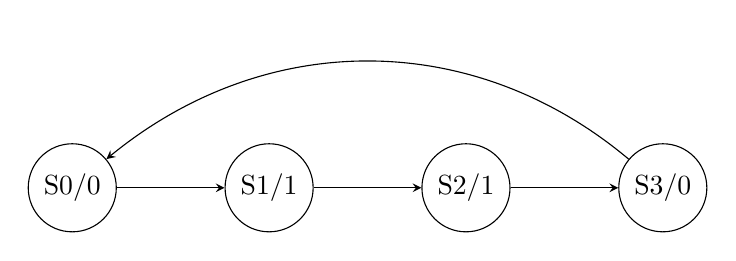
\begin{tikzpicture}[->, >=stealth, node distance=2.5cm, auto]
  \node[draw, circle] (S0) at (0,0) {S0/0};
  \node[draw, circle] (S1) at (2.5,0) {S1/1};
  \node[draw, circle] (S2) at (5,0) {S2/1};
  \node[draw, circle] (S3) at (7.5,0) {S3/0};

  \draw (S0) -- (S1);
  \draw (S1) -- (S2);
  \draw (S2) -- (S3);
  \draw (S3) edge[bend right=40] (S0);
\end{tikzpicture}
\end{center}

\begin{lstlisting}[caption={序列0110发生器（状态机版本）}]
architecture fsm of seq_gen_0110 is
  type state_type is (S0, S1, S2, S3);
  signal state : state_type;
begin
  process(clk, rst_n)
  begin
    if rst_n = '0' then
      state <= S0;
    elsif rising_edge(clk) then
      case state is
        when S0 => state <= S1;
        when S1 => state <= S2;
        when S2 => state <= S3;
        when S3 => state <= S0;
      end case;
    end if;
  end process;

  -- 输出逻辑
  seq_out <= '0' when (state = S0 or state = S3) else '1';
end fsm;
\end{lstlisting}

\section{方案3：移位寄存器型序列发生器}

有些序列恰好可以用移位寄存器+反馈产生。例如伪随机序列（LFSR）。

这将在第六部分（移位寄存器）和第七部分（环形计数器）中详细展开。

\section{方案4：ROM/查找表型序列发生器}

适用于长序列：
\begin{itemize}
  \item 将整个序列预存在ROM中
  \item 计数器作为ROM的地址
  \item ROM输出 = 序列值
\end{itemize}

\section{方案比较}

\begin{center}
\begin{tabular}{|l|c|c|c|}
\hline
\textbf{方案} & \textbf{适用场景} & \textbf{优点} & \textbf{缺点} \\
\hline
计数器+MUX & 序列有规律 & 资源少 & 需要推导逻辑 \\
状态机 & 任意序列 & 通用 & 状态多时复杂 \\
移位寄存器 & LFSR/循环型 & 结构规整 & 仅限特定类型 \\
ROM/查找表 & 长序列 & 通用 & 资源多（需要ROM） \\
\hline
\end{tabular}
\end{center}

\section{考试常见变式}

\begin{enumerate}
  \item \textbf{变式1：设计任意周期性的序列}

  例：产生序列 10110 10110 ...（长度5）
  解：模5计数器 + 状态到输出映射表

  \item \textbf{变式2：多路输出序列}

  同时输出多个相关序列（如正交序列）

  \item \textbf{变式3：伪随机序列（LFSR）}

  用移位寄存器+反馈产生看似随机的序列。这是通信系统中的重要应用。

  \item \textbf{变式4：可配置的序列发生器}

  序列可以动态改变（通过改变映射表或ROM内容）
\end{enumerate}

\begin{examtip}[序列发生器秒杀法]
1. 确定序列长度L
2. 设计模L计数器
3. 建立状态→输出映射表（真值表）
4. 推导输出逻辑（或用case直接写）

\textbf{计数器+case语句是最通用的解法，适用于任何序列。}
\end{examtip}

\section{变式详解}
\chapter{序列发生器——全部变式详解}

\section{变式1：任意周期序列（计数器+映射表）}

\begin{detailbox}[完整教学]
\textbf{【通用方案】}模L计数器+状态→输出映射表。
\textbf{【例题】}产生序列10110(长度5)。模5计数器+case映射：
\begin{lstlisting}
case cnt is
  when "000" => seq <= '1';
  when "001" => seq <= '0';
  when "010" => seq <= '1';
  when "011" => seq <= '1';
  when "100" => seq <= '0';
end case;
\end{lstlisting}
\textbf{【适用范围】}任意序列。长度L→模L计数器。
\end{detailbox}


\section{变式2：状态机型序列发生器}

\begin{detailbox}[完整教学]
\textbf{【方案】}每个状态输出一个序列值。状态转移=序列顺序。
\textbf{【优点】}状态名有意义（如"S\_1","S\_0","S\_1","S\_1","S\_0"）。但状态多时代码冗长。
\textbf{【比较】}推荐用计数器+case——代码更简洁。
\end{detailbox}


\section{变式3：移位寄存器+LFSR发生器}

\begin{detailbox}[完整教学]
\textbf{【LFSR】}线性反馈移位寄存器。反馈=选择位的XOR。
\textbf{【应用】}伪随机序列(PRBS)、CRC、扰码。
\textbf{【4位LFSR(X4+X3+1)】}反馈=Q3 xor Q2。产生15个伪随机状态。
\textbf{【注意】}全0状态非法——LFSR会锁死在0000。必须初始化为非0值。
\end{detailbox}


\section{变式4：ROM/查找表型序列发生器}

\begin{detailbox}[完整教学]
\textbf{【方案】}预存整个序列在ROM中。计数器=地址。
\textbf{【优点】}任意序列、可重配置。适合长序列。
\textbf{【VHDL】}
\begin{lstlisting}
type rom_type is array (0 to 15) of std_logic_vector(3 downto 0);
constant SEQ_ROM : rom_type := (x"1", x"0", x"1", x"1", x"0", ...);
seq <= SEQ_ROM(to_integer(unsigned(cnt)));
\end{lstlisting}
\end{detailbox}


% =============================================================
%  第六部分：移位寄存器体系
% =============================================================
\part{移位寄存器体系}

\chapter{移位寄存器}

\section{先建立数据流动的思维模型}

回顾D触发器：一个D触发器在时钟上升沿采样D输入，输出到Q。

现在把\textbf{多个D触发器首尾连接}：

\begin{center}
\begin{tikzpicture}
  \node[draw, minimum width=1.2cm, minimum height=1.5cm, label=above:DFF0] (dff0) at (0,0) {};
  \node[draw, minimum width=1.2cm, minimum height=1.5cm, label=above:DFF1] (dff1) at (2,0) {};
  \node[draw, minimum width=1.2cm, minimum height=1.5cm, label=above:DFF2] (dff2) at (4,0) {};
  \node[draw, minimum width=1.2cm, minimum height=1.5cm, label=above:DFF3] (dff3) at (6,0) {};

  \draw[->] (dff0.east) -- (dff1.west) node[midway,above] {Q0=D1};
  \draw[->] (dff1.east) -- (dff2.west) node[midway,above] {Q1=D2};
  \draw[->] (dff2.east) -- (dff3.west) node[midway,above] {Q2=D3};

  \node (din) at (-2,0) {$D_{in}$};
  \draw[->] (din) -- (dff0.west);
  \node (dout) at (8,0) {$Q_3$};
  \draw[->] (dff3.east) -- (dout);

  \node at (3,-1.5) {每个D触发器的Q接到下一个D触发器的D};
\end{tikzpicture}
\end{center}

\begin{keypoint}[移位寄存器的核心结构]
移位寄存器 = N个D触发器串联

$$\text{DFF}_k \text{的} Q \to \text{DFF}_{k+1} \text{的} D$$

在时钟上升沿，每个DFF采样前一级DFF的Q输出。
结果：\textbf{所有数据同时向右移动一位。}
\end{keypoint}

\section{逐拍分析：数据如何移动}

这是全书最重要的状态分析之一。请仔细跟着每一拍。

\subsection{初始条件}

假设4个D触发器初始值：Q3Q2Q1Q0 = 0000

串行输入 $D_{in}$ 序列：1, 0, 1, 1, 0, ...

（每个时钟周期，一个新的$D_{in}$值被送入最左边的DFF0）

\subsection{时钟第0拍（初始状态）}

\begin{itemize}
  \item 寄存器内容：Q3=0, Q2=0, Q1=0, Q0=0 → [0 0 0 0]
  \item 当前$D_{in}$ = 1（准备好，等待下一个上升沿）
\end{itemize}

\subsection{时钟第1拍上升沿}

\begin{beatanalysis}[移位寄存器——时钟第1拍]
\textbf{上升沿到达时发生的事情（所有DFF同时动作）：}

\begin{center}
\begin{tabular}{|c|c|c|c|c|}
\hline
\textbf{DFF} & \textbf{D输入(上升沿前)} & \textbf{上升沿后Q} & \textbf{DFF动作} \\
\hline
DFF0 & $D_{in}$=1 & Q0=\textbf{1} & 采样外部输入1 \\
DFF1 & Q0=0 & Q1=\textbf{0} & 采样前一拍Q0的值(0) \\
DFF2 & Q1=0 & Q2=\textbf{0} & 采样前一拍Q1的值(0) \\
DFF3 & Q2=0 & Q3=\textbf{0} & 采样前一拍Q2的值(0) \\
\hline
\end{tabular}

\textbf{上升沿后寄存器内容：[0 0 0 1]}（1进入最右端）

原来在Q0的0移到了Q1，原来在Q1的0移到了Q2，原来在Q2的0移到了Q3。
Q3原来的值（0）被"挤出去"了——这就是串行输出。
\end{center}
\end{beatanalysis}

\subsection{时钟第2拍上升沿}

现在 $D_{in}$ = 0

\begin{beatanalysis}[移位寄存器——时钟第2拍]
\begin{center}
\begin{tabular}{|c|c|c|c|c|}
\hline
\textbf{DFF} & \textbf{D输入(上升沿前)} & \textbf{上升沿后Q} & \textbf{DFF动作} \\
\hline
DFF0 & $D_{in}$=0 & Q0=\textbf{0} & 采样外部输入0 \\
DFF1 & Q0=1 & Q1=\textbf{1} & 采样Q0的值(1) → 1右移 \\
DFF2 & Q1=0 & Q2=\textbf{0} & 采样Q1的值(0) → 0右移 \\
DFF3 & Q2=0 & Q3=\textbf{0} & 采样Q2的值(0) → 0右移 \\
\hline
\end{tabular}

\textbf{上升沿后寄存器内容：[0 0 1 0]}（之前Q0的1现在移到了Q1）
\end{center}
\end{beatanalysis}

\subsection{时钟第3拍上升沿}

现在 $D_{in}$ = 1

\begin{beatanalysis}[移位寄存器——时钟第3拍]
\begin{center}
\begin{tabular}{|c|c|c|c|c|}
\hline
\textbf{DFF} & \textbf{D输入(上升沿前)} & \textbf{上升沿后Q} & \textbf{说明} \\
\hline
DFF0 & $D_{in}$=1 & Q0=\textbf{1} & 新数据进入 \\
DFF1 & Q0=0 & Q1=\textbf{0} & \\
DFF2 & Q1=1 & Q2=\textbf{1} & 1继续右移 \\
DFF3 & Q2=0 & Q3=\textbf{0} & \\
\hline
\end{tabular}

\textbf{上升沿后寄存器内容：[0 1 0 1]}（可以看到1在向右移动！）
\end{center}
\end{beatanalysis}

\subsection{时钟第4拍上升沿}

现在 $D_{in}$ = 1

\textbf{上升沿后寄存器内容：[1 0 1 1]}

\subsection{完整数据移动轨迹}

\begin{center}
\begin{tabular}{|c|c|c|c|c|c|}
\hline
\textbf{时钟拍} & \textbf{$D_{in}$} & \textbf{Q3} & \textbf{Q2} & \textbf{Q1} & \textbf{Q0} \\
\hline
0（初始）& — & 0 & 0 & 0 & 0 \\
1 & 1 & 0 & 0 & 0 & \textbf{1} \\
2 & 0 & 0 & 0 & \textbf{1} & 0 \\
3 & 1 & 0 & \textbf{1} & 0 & 1 \\
4 & 1 & \textbf{1} & 0 & 1 & 1 \\
5 & 0 & \textbf{0} & 1 & 1 & 0 \\
\hline
\end{tabular}
\end{center}

\textbf{观察数据流：}每个1从$D_{in}$进入，经过4个时钟周期后从Q3串行输出。

就像水管中的水流——从一端进入，经过管道，从另一端流出。

\section{核心概念总结}

\begin{enumerate}
  \item \textbf{串行输入（Serial In）}：数据从最左边的DFF一个bit一个bit地进入
  \item \textbf{串行输出（Serial Out）}：数据从最右边的DFF一个bit一个bit地流出
  \item \textbf{并行输出（Parallel Out）}：所有Q值同时观察——看到"管道"中当前的内容
  \item \textbf{并行输入（Parallel Load）}：直接设置所有DFF的值（跳过移位过程）
\end{enumerate}

\section{单向移位寄存器：VHDL实现}

\begin{lstlisting}[caption={4位右移移位寄存器（串入串出/并出）}]
library ieee;
use ieee.std_logic_1164.all;

entity shift_reg_right is
  port (
    clk     : in  std_logic;
    rst_n   : in  std_logic;
    si      : in  std_logic;  -- 串行输入
    so      : out std_logic;  -- 串行输出
    po      : out std_logic_vector(3 downto 0)  -- 并行输出
  );
end shift_reg_right;

architecture behavioral of shift_reg_right is
  signal reg : std_logic_vector(3 downto 0);
begin
  process(clk, rst_n)
  begin
    if rst_n = '0' then
      reg <= (others => '0');
    elsif rising_edge(clk) then
      reg <= si & reg(3 downto 1);  -- 右移：新数据进最高位
    end shift;
  end process;

  so <= reg(0);  -- 串行输出 = 最低位
  po <= reg;     -- 并行输出 = 整个寄存器
end behavioral;
\end{lstlisting}

\textbf{关键语句}：\texttt{reg <= si \& reg(3 downto 1)}

这表示：
\begin{itemize}
  \item reg(3)（原来的最高位）$\to$ reg(2)
  \item reg(2) $\to$ reg(1)
  \item reg(1) $\to$ reg(0)
  \item si（新数据）$\to$ reg(3)
\end{itemize}

数据向右移动一位。新数据从左边进入，最右边的数据（reg(0)）被挤出。

\section{双向移位寄存器}

双向 = 既可以左移也可以右移，由方向控制信号决定。

\begin{lstlisting}[caption={双向移位寄存器}]
library ieee;
use ieee.std_logic_1164.all;

entity shift_reg_bidir is
  port (
    clk     : in  std_logic;
    rst_n   : in  std_logic;
    dir     : in  std_logic;  -- 方向：'1'=右移, '0'=左移
    si      : in  std_logic;  -- 串行输入
    po      : out std_logic_vector(3 downto 0)
  );
end shift_reg_bidir;

architecture behavioral of shift_reg_bidir is
  signal reg : std_logic_vector(3 downto 0);
begin
  process(clk, rst_n)
  begin
    if rst_n = '0' then
      reg <= (others => '0');
    elsif rising_edge(clk) then
      if dir = '1' then
        reg <= si & reg(3 downto 1);  -- 右移
      else
        reg <= reg(2 downto 0) & si;  -- 左移
      end if;
    end if;
  end process;

  po <= reg;
end behavioral;
\end{lstlisting}

\section{带并行装载的移位寄存器}

增加一个load信号，允许直接设置所有D触发器的值：

\begin{lstlisting}[caption={带并行装载的移位寄存器}]
library ieee;
use ieee.std_logic_1164.all;

entity shift_reg_load is
  port (
    clk     : in  std_logic;
    rst_n   : in  std_logic;
    load    : in  std_logic;  -- 并行装载使能
    data_in : in  std_logic_vector(3 downto 0);  -- 并行输入
    si      : in  std_logic;  -- 串行输入
    po      : out std_logic_vector(3 downto 0)
  );
end shift_reg_load;

architecture behavioral of shift_reg_load is
  signal reg : std_logic_vector(3 downto 0);
begin
  process(clk, rst_n)
  begin
    if rst_n = '0' then
      reg <= (others => '0');
    elsif rising_edge(clk) then
      if load = '1' then
        reg <= data_in;  -- 并行装载
      else
        reg <= si & reg(3 downto 1);  -- 右移
      end if;
    end if;
  end process;

  po <= reg;
end behavioral;
\end{lstlisting}

\section{四种输入输出组合}

\begin{center}
\begin{tabular}{|l|l|l|l|}
\hline
\textbf{类型} & \textbf{输入方式} & \textbf{输出方式} & \textbf{典型应用} \\
\hline
SISO & 串行入 & 串行出 & 延迟线 \\
SIPO & 串行入 & 并行出 & 串并转换 \\
PISO & 并行入 & 串行出 & 并串转换 \\
PIPO & 并行入 & 并行出 & 通用寄存器 \\
\hline
\end{tabular}
\end{center}

SISO = Serial In Serial Out（串入串出）
SIPO = Serial In Parallel Out（串入并出）
PISO = Parallel In Serial Out（并入串出）
PIPO = Parallel In Parallel Out（并入并出）

\section{移位寄存器实现分频器}

\subsection{基本原理}

移位寄存器天然具有分频能力。回顾环形计数器和Johnson计数器：

\begin{itemize}
  \item N位环形计数器：N个状态循环，任何Q输出的频率 = $f_{clk} / N$
  \item N位Johnson计数器：2N个状态循环，任何Q输出的频率 = $f_{clk} / (2N)$
\end{itemize}

因为移位寄存器中的"1"（或状态模式）每N拍（或2N拍）才经过同一个触发器一次，所以每个Q输出的翻转频率恰好是时钟的$1/N$（或$1/2N$）。

\subsection{逐拍分析：4位环形计数器做4分频}

假设4位环形计数器初始状态1000，反馈Q0$\to$D3（闭环）。

\begin{center}
\begin{tabular}{|c|c|c|c|c|c|}
\hline
时钟拍 & Q3 & Q2 & Q1 & Q0 & 说明 \\
\hline
0 & 1 & 0 & 0 & 0 & 初始 \\
1 & 0 & 1 & 0 & 0 & 1右移 \\
2 & 0 & 0 & 1 & 0 & \\
3 & 0 & 0 & 0 & 1 & \\
4 & 1 & 0 & 0 & 0 & 回到初始！\\
\hline
\end{tabular}
\end{center}

Q3的输出序列：1, 0, 0, 0, 1, 0, 0, 0, ...
周期 = 4个时钟 $\to$ 频率 = $f_{clk} / 4$。

\textbf{每个Q输出都是4分频信号，只是相位不同。}

\subsection{Johnson计数器做分频器}

4位Johnson计数器（8状态）：
$$0000\to1000\to1100\to1110\to1111\to0111\to0011\to0001\to0000$$

任意Q输出的周期 = 8个时钟 $\to$ 频率 = $f_{clk} / 8$。

\textbf{规律：}N位Johnson计数器 = $2N$分频（所有Q输出频率相同，相位不同）。

\subsection{VHDL实现：移位寄存器型分频器}

\begin{lstlisting}[caption={4位环形计数器做4分频器}]
library ieee;
use ieee.std_logic_1164.all;

entity shift_div4 is
  port(
    clk, rst : in  std_logic;
    clk_out  : out std_logic
  );
end shift_div4;

architecture behav of shift_div4 is
  signal reg : std_logic_vector(3 downto 0);
begin
  process(clk, rst)
  begin
    if rst = '1' then reg <= "1000";
    elsif rising_edge(clk) then
      reg <= reg(0) & reg(3 downto 1);
    end if;
  end process;
  clk_out <= reg(3);  -- Q3 = 4分频输出
end behav;
\end{lstlisting}

\subsection{与计数器分频的对比}

\begin{center}
\begin{tabular}{|l|c|c|}
\hline
\textbf{分频方式} & \textbf{结构} & \textbf{可得分频比} \\
\hline
二进制计数器取Qn & 加法器+寄存器 & $2^n$（Q0=2, Q1=4, Q2=8...）\\
环形计数器 & N个DFF+反馈 & N（4位$\to$4分频）\\
Johnson计数器 & N个DFF+反相反馈 & 2N（4位$\to$8分频）\\
模M计数器+比较 & 加法器+寄存器+比较器 & 任意M \\
\hline
\end{tabular}
\end{center}

\textbf{移位寄存器分频的优缺点：}
\begin{itemize}
  \item 优点：结构规整（只有D触发器和反馈线），关键路径极短（1级DFF延迟），适合超高速分频
  \item 缺点：分频比固定（N或2N），灵活性不如计数器方案
\end{itemize}

\section{移位寄存器实现序列发生器}

\subsection{方法一：循环移位型（只能循环输出初值，不是真正的序列发生器）}

\textbf{先说清楚：这不是真正的序列发生器。}它只是把装进去的值循环输出——装1001就循环出1001，装0101就循环出0101。你无法用它"设计"出一个新的序列。

那为什么还要讲？因为\textbf{硬件结构}和真正的序列发生器一模一样：都是移位寄存器+反馈线。理解了循环移位，查表法就水到渠成。

\textbf{方案：}移位寄存器 + 反馈逻辑（Q0直接反馈给D3）。每拍数据右移一位，最低位移回最高位。

\textbf{例题：}4位寄存器，反馈 = Q0→D3，初值"1001"。

\begin{center}
\begin{tabular}{|c|c|c|c|c|}
\hline
时钟拍 & Q3 & Q2 & Q1 & Q0 \\
\hline
0 & 1 & 0 & 0 & 1（初始）\\
1 & 1 & 1 & 0 & 0（Q0=1反馈到D3）\\
2 & 0 & 1 & 1 & 0 \\
3 & 0 & 0 & 1 & 1 \\
4 & 1 & 0 & 0 & 1（回到初始！）\\
\hline
\end{tabular}
\end{center}

序列长度 = 4拍。输出就是初值本身，循环重复。\textbf{这不是序列"生成"，只是"循环播放"。}

\textbf{【VHDL——循环右移序列发生器】}
\begin{lstlisting}
library ieee;
use ieee.std_logic_1164.all;

entity shift_seq_gen is
  port(clk, rst : in std_logic; seq_out : out std_logic_vector(3 downto 0));
end shift_seq_gen;

architecture behav of shift_seq_gen is
  signal reg : std_logic_vector(3 downto 0);
begin
  process(clk, rst)
  begin
    if rst='1' then reg <= "1001";
    elsif rising_edge(clk) then
      reg <= reg(0) & reg(3 downto 1);  -- 循环右移
    end if;
  end process;
  seq_out <= reg;
end behav;
\end{lstlisting}

\subsection{方法二：查表反馈型（通用序列发生器）}

循环移位只能产生移位相关的序列。要产生\textbf{任意序列}，需要用查表法（CASE语句）根据当前状态决定反馈值。

\textbf{核心结构：}移位寄存器 + CASE查表器。CASE根据寄存器的当前值，查表输出下一位要移入的din值。

\subsection{例题：用3位移位寄存器产生序列 00011101 00011101...}

\textbf{设计分析：}3位移位寄存器共8个状态，每个状态通过CASE指定反馈位din的值。输出取寄存器最高位q(2)。

\subsection{核心问题：CASE表是怎么得到的？}

这是初学者最容易困惑的地方。答案：\textbf{用3位滑动窗口在目标序列上滑动}。

目标序列是：0 0 0 1 1 1 0 1（周期8，循环重复）。

\begin{center}
\begin{tikzpicture}[scale=0.9]
% Target sequence
\node at (0, 2.5) {目标序列(循环):};
\foreach \i/\b in {0/0,1/0,2/0,3/1,4/1,5/1,6/0,7/1} {
  \node at (\i*1.2, 2) {\b};
}
% Window 0
\draw[red,very thick] (-0.3,1.5) rectangle (2.1,1.0);
\node[red] at (0.9, 1.25) {窗口0: 000};
\node[red] at (3.3, 1.25) {$\to$ 下一个是1 $\to$ din='1'};
\node[red] at (3.3, 0.75) {$\to$ state="000"};

% Window 1
\draw[blue,very thick] (0.9,1.5) rectangle (3.3,1.0);
\node[blue] at (2.1, 0.5) {窗口1: 001 $\to$ 下一个1 $\to$ din='1'};

% Window 2
\draw[green!50!black,very thick] (2.1,1.5) rectangle (4.5,1.0);
\node[green!50!black] at (3.3, 0.5) {窗口2: 011 $\to$ 下一个1 $\to$ din='1'};

% Window 3
\draw[orange,very thick] (3.3,1.5) rectangle (5.7,1.0);
\node[orange] at (4.5, 0.5) {窗口3: 111 $\to$ 下一个0 $\to$ din='0'};

% Ellipsis
\node at (6.5, 0.5) {...};
\end{tikzpicture}
\end{center}

\textbf{推导步骤：}

\begin{enumerate}
\item 把目标序列写成循环：\textbf{0 0 0 1 1 1 0 1 | 0 0 0 1 1 1 0 1 | ...}（首尾相接，无限重复）
\item 用宽度为3的窗口，从序列开头每次移动一位，读取窗口内的3个bit——这就是3个D触发器的\textbf{当前状态}
\item 窗口右边紧挨着的下一个bit——就是需要反馈进入的\textbf{din值}
\item 覆盖所有8种可能的3-bit组合（因为3位有$2^3=8$种组合，恰好一个周期遍历完）
\end{enumerate}

\textbf{图解推导——3位滑动窗口法：}

\begin{center}
\begin{tabular}{cccccccccccccccccccc}
\multicolumn{20}{c}{目标序列（无限循环，用竖线标出8个3位窗口）} \\
& & & \fbox{0 0 0} & 1 & 1 & 1 & 0 & 1 & 0 & 0 & 0 & 1 & ... & $\leftarrow$ 窗口0: state=000, din=1 \\
& & 0 & \fbox{0 0 1} & 1 & 1 & 0 & 1 & 0 & 0 & 0 & 1 & ... & & $\leftarrow$ 窗口1: state=001, din=1 \\
& 0 & 0 & \fbox{0 1 1} & 1 & 0 & 1 & 0 & 0 & 0 & 1 & ... & & & $\leftarrow$ 窗口2: state=011, din=1 \\
0 & 0 & 0 & \fbox{1 1 1} & 0 & 1 & 0 & 0 & 0 & 1 & ... & & & & $\leftarrow$ 窗口3: state=111, din=0 \\
0 & 0 & 0 & 1 & \fbox{1 1 0} & 1 & 0 & 0 & 0 & 1 & ... & & & & $\leftarrow$ 窗口4: state=110, din=1 \\
0 & 0 & 0 & 1 & 1 & \fbox{1 0 1} & 0 & 0 & 0 & 1 & ... & & & & $\leftarrow$ 窗口5: state=101, din=0 \\
0 & 0 & 0 & 1 & 1 & 1 & \fbox{0 1 0} & 0 & 0 & 1 & ... & & & & $\leftarrow$ 窗口6: state=010, din=0 \\
0 & 0 & 0 & 1 & 1 & 1 & 0 & \fbox{1 0 0} & 0 & 1 & ... & & & & $\leftarrow$ 窗口7: state=100, din=0 \\
\end{tabular}
\end{center}

\textbf{关键理解：}
\begin{itemize}
  \item \fbox{框内3位} = 3个D触发器的当前状态 (qin)
  \item 框右边紧跟着的bit = 下一个要移入的din值
  \item 框最左边的bit = 当前输出值 (Q2)
  \item 下一个时钟沿：din从右边移入，所有bit左移一位 → 窗口向右滑动一位 → Q2输出下一个bit
\end{itemize}

\subsection{关键技巧：需要几个D触发器？——试3个不行就换4个}

\textbf{窗口宽度 = 寄存器的个数。}窗口太窄，不同位置的窗口值会重复（"撞车"），导致CASE表出现矛盾——同一个状态对应两个不同的din值。

\textbf{举例：序列 00110011...（8位循环），先试3位窗口}

\[
\underbrace{001}_{\text{窗口0}}10011\underbrace{001}_{\text{窗口4}}10011...
\]

\begin{center}
\begin{tabular}{c|c|c}
窗口位置 & 窗口值(3位) & 下一个bit(din) \\
\hline
0 & 001 & 1 \\
1 & 011 & 0 \\
2 & 110 & 0 \\
3 & 100 & 1 \\
4 & 001 & \textbf{？} ← 窗口值=001又出现了！但这次下一个bit是1？0？\\
\end{tabular}
\end{center}

窗口0（001）的下一个是1，窗口4（001）的下一个本来是接着序列...但\textbf{同一个状态"001"在CASE表中只能有一行}，不能同时对应din=1和din=0。这就是"撞车"。

\textbf{解决方案：窗口加宽→换4个寄存器}

\begin{center}
\begin{tabular}{c|c|c}
窗口位置 & 窗口值(4位) & 下一个bit(din) \\
\hline
0 & 0011 & 0 \\
1 & 0110 & 0 \\
2 & 1100 & 1 \\
3 & 1001 & 1 \\
4 & 0011 & 0 ← 和窗口0一样！但下一个bit也一样(都是0)，不冲突 ✓ \\
\end{tabular}
\end{center}

4位窗口下，0011→下一个是0，再次出现0011时下一个还是0，\textbf{CASE表不矛盾}。

\textbf{通用法则：}

\begin{keypoint}[寄存器位数的确定]
\textbf{先试$k = \lceil\log_2 L\rceil$位（L=序列长度），用滑动窗口检查有没有"撞车"。}

\begin{itemize}
  \item 8种窗口值全不同 → $k$位够用
  \item 有重复但重复处的din也相同 → $k$位够用
  \item 有重复且din不同 → \textbf{窗口加宽为$k+1$位，重新检查}
\end{itemize}

选最小不撞车的位数作为寄存器个数。
\end{keypoint}

\subsection{完整例题：你需要几个寄存器？}

\textbf{题目：用查表法产生序列 0011001 0011001...（7位循环），最少需要几个D触发器？}

\textbf{第一步：算起步位数} $\lceil\log_2 7\rceil = 3$位。\textbf{先用3位窗口试。}

把序列循环展开写两遍，方便看环绕：0 0 1 1 0 0 1 | 0 0 1 1 0 0 1

\begin{center}
\begin{tabular}{c|c|c}
位置 & 3位窗口值(qin) & 右边一个bit(din) \\
\hline
0 & 001 & \textbf{1} \\
1 & 011 & \textbf{0} \\
2 & 110 & \textbf{0} \\
3 & 100 & \textbf{0} \\
4 & 001 & \textbf{0} ？\\
5 & 010 & \textbf{0} \\
6 & 100 & \textbf{1} ？\\
\hline
\end{tabular}
\end{center}

\textbf{查撞车：}
\begin{itemize}
  \item 位置0的001 → din=1，位置4的001 → din=0。\textbf{同一个001，din不同！撞车！}
  \item 位置3的100 → din=0，位置6的100 → din=1。\textbf{又撞车！}
\end{itemize}

3位不行→\textbf{换4位窗口。}

\textbf{第二步：4位窗口}

序列：0 0 1 1 0 0 1 | 0 0 1 1 0 0 1

\begin{center}
\begin{tabular}{c|c|c}
位置 & 4位窗口值(qin) & 下一个bit(din) \\
\hline
0 & 0011 & 0 \\
1 & 0110 & 0 \\
2 & 1100 & 1 \\
3 & 1001 & 0 \\
4 & 0010 & 0 \\
5 & 0100 & 1 \\
6 & 1001 & \textbf{1} ？\\
\hline
\end{tabular}
\end{center}

位置3(1001)→din=0，位置6(1001)→din=1。\textbf{还是撞！}→ 换5位。

\textbf{第三步：5位窗口}

\begin{center}
\begin{tabular}{c|c|c}
位置 & 5位窗口值(qin) & 下一个bit(din) \\
\hline
0 & 00110 & 0 \\
1 & 01100 & 1 \\
2 & 11001 & 0 \\
3 & 10010 & 0 \\
4 & 00100 & 1 \\
5 & 01001 & 0 \\
6 & 10011 & (回0)0 \\
\hline
\end{tabular}
\end{center}

\textbf{7个5位窗口全部不同！}→ 需要\textbf{5个寄存器}。

\textbf{结论：}$\lceil\log_2 7\rceil = 3$只是理论下界。实际寄存器数取决于序列本身的结构——有些序列3位够用（如00011101），有些需要更多（如0011001需要5位）。\textbf{试到不撞车为止。}

\subsection{速查：多少位寄存器够用？}

\begin{center}
\begin{tabular}{|c|c|c|c|}
\hline
序列长度L & $\lceil\log_2 L\rceil$（起步） & 最坏需要 & 常见需要 \\
\hline
4 & 2 & 2 & 2 \\
5 & 3 & 3 & 3 \\
6 & 3 & 3$\sim$4 & 3 \\
7 & 3 & 5 & 3$\sim$4 \\
8 & 3 & 3 & 3 \\
\hline
\end{tabular}
\end{center}

\textbf{考试做法：}先用$\lceil\log_2 L\rceil$位，画滑动窗口表，检查有无撞车（同一窗口值对应不同din）。不撞→够用；撞→加一位重新画。

\subsection{VHDL实现：5位寄存器产生序列0011001}

5位寄存器共$2^5=32$种可能状态，但循环只经过7个。CASE只写这7个合法状态，其余25个状态统一扔到when others回初始态。

\begin{lstlisting}
library IEEE;
use IEEE.STD_LOGIC_1164.all;

entity seqgen_5bit is
  port(clk, rst : in std_logic; q : out std_logic);
end seqgen_5bit;

architecture behav of seqgen_5bit is
  signal qin : std_logic_vector(4 downto 0);
  signal din : std_logic;
begin
  -- 查表产生反馈位din
  process(clk)
  begin
    if rising_edge(clk) then
      case qin is
        when "00110" => din <= '0';
        when "01100" => din <= '1';
        when "11001" => din <= '0';
        when "10010" => din <= '0';
        when "00100" => din <= '1';
        when "01001" => din <= '0';
        when "10011" => din <= '0';
        when others  => din <= '0';  -- 非法状态兜底
      end case;
    end if;
  end process;

  -- 移位寄存器：左移，din进入最低位
  process(clk, rst)
  begin
    if rst = '1' then
      qin <= "00110";  -- 初始窗口0
    elsif rising_edge(clk) then
      qin <= qin(3 downto 0) & din;
    end if;
  end process;

  q <= qin(4);  -- 输出最高位
end behav;
\end{lstlisting}

\textbf{逐拍验证：}
\begin{center}
\begin{tabular}{|c|c|c|c|}
\hline
拍 & qin(当前) & din & q(输出)=qin(4) \\
\hline
0 & 00110 & 0 & 0 \\
1 & 01100 & 1 & 0 \\
2 & 11001 & 0 & 1 \\
3 & 10010 & 0 & 1 \\
4 & 00100 & 1 & 0 \\
5 & 01001 & 0 & 0 \\
6 & 10011 & 0 & 1 \\
7 & 00110 & — & 0 ← 回到拍0 \\
\hline
\end{tabular}
\end{center}

输出 q：0,0,1,1,0,0,1,0,0,1,1,0,0,1,... ← 确实就是0011001循环。

\textbf{这就是CASE表的来源：}不撞车的窗口值→下一个bit，整理成表。

\textbf{这就是CASE表的来源：}把上面8个窗口的"窗口值→下一个bit"整理成表，就是CASE表。

\textbf{完整CASE表推导：}
\begin{center}
\begin{tabular}{|c|c|c|c|c|}
\hline
窗口编号 & 窗口内容(qin) & 窗口右边bit(din) & 下一拍qin(左移后) & 输出q(2) \\
\hline
0 & 000 & \textbf{1} & 001 & 0 \\
1 & 001 & \textbf{1} & 011 & 0 \\
2 & 011 & \textbf{1} & 111 & 0 \\
3 & 111 & \textbf{0} & 110 & 1 \\
4 & 110 & \textbf{1} & 101 & 1 \\
5 & 101 & \textbf{0} & 010 & 1 \\
6 & 010 & \textbf{0} & 100 & 0 \\
7 & 100 & \textbf{0} & 000 & 1 \\
\hline
\end{tabular}
\end{center}

\textbf{逐拍追踪：}
\begin{center}
\begin{tabular}{|c|c|c|c|c|}
\hline
时钟拍 & qin(当前) & CASE查表→din & 下一拍qin & 输出q(2) \\
\hline
0 & 000 & 1 & 001 & 0 \\
1 & 001 & 1 & 011 & 0 \\
2 & 011 & 1 & 111 & 0 \\
3 & 111 & 0 & 110 & 1 \\
4 & 110 & 1 & 101 & 1 \\
5 & 101 & 0 & 010 & 1 \\
6 & 010 & 0 & 100 & 0 \\
7 & 100 & 0 & 000 & 1 \\
8 & 000 & — & — & 回到拍0 \\
\hline
\end{tabular}
\end{center}

输出序列 q(2)：0,0,0,1,1,1,0,1,0,0,0,1,1,1,0,1,... 周期=8。\textbf{与目标序列完全一致！}

\textbf{【VHDL——查表反馈型序列发生器】}
\begin{lstlisting}
library IEEE;
use IEEE.STD_LOGIC_1164.all;

entity seqgen_table is
  port(clk, rst : in std_logic; q : out std_logic);
end seqgen_table;

architecture behav of seqgen_table is
  signal qin : std_logic_vector(2 downto 0);
  signal din : std_logic;
begin
  -- 第一段：CASE查表产生反馈位din
  comb_proc: process(clk)
  begin
    if rising_edge(clk) then
      case qin is
        when "000" => din <= '1';
        when "001" => din <= '1';
        when "011" => din <= '1';
        when "111" => din <= '0';
        when "110" => din <= '1';
        when "101" => din <= '0';
        when "010" => din <= '0';
        when "100" => din <= '0';
        when others => din <= '0';
      end case;
    end if;
  end process;

  -- 第二段：移位寄存器（左移，din进入最低位）
  shift_proc: process(clk, rst)
  begin
    if rst = '1' then qin <= (others => '0');
    elsif rising_edge(clk) then
      qin <= qin(1 downto 0) & din;
    end if;
  end process;

  q <= qin(2);  -- 输出最高位
end behav;
\end{lstlisting}

\textbf{【设计思想】}查表法的本质：把想要的序列"写死"在CASE表里。当前状态→查表→下一个输入位。只要改CASE表的内容，就能生成任何8位循环序列。这是\textbf{通用序列发生器}的设计范式。

\subsection{两种方案对比}

\begin{center}
\begin{tabular}{|l|c|c|}
\hline
\textbf{方案} & \textbf{循环移位型} & \textbf{查表反馈型} \\
\hline
反馈逻辑 & reg(0) $\to$ D(N-1)（一根线） & CASE表（多条件判断） \\
序列来源 & 就是初值本身（装入什么输出什么）& CASE表任意指定（真正的设计）\\
代码复杂度 & 1行 & N行（每个状态1行）\\
修改序列 & 改初值（但只能输出初值循环）& 修改CASE表内容（任意序列）\\
适用场景 & 学习移位寄存器工作原理 & 实际的序列发生器设计 \\
\hline
\end{tabular}
\end{center}

\section{移位寄存器实现串行加法器}

\subsection{原理}

并行加法器（如行波进位）一次完成所有位的加法。串行加法器逐位相加，每次处理1位，N拍后得到N位结果。\textbf{核心结构：}1位全加器 + 进位D触发器 + 两个移位寄存器（存放操作数A和B）+ 一个移位寄存器（存放结果）。

\subsection{逐拍工作过程}

以4位加法 1011 + 0110 为例：

\begin{center}
\begin{tabular}{|c|c|c|c|c|c|}
\hline
拍 & A移位器(Q0) & B移位器(Q0) & Cin(DFF) & Sum位 & Cout \\
\hline
0（初）& 1 & 0 & 0 & — & — \\
1 & 1 & 0 & 0 & 1 & 0 \\
2 & 1 & 1 & 0 & 0 & 1 \\
3 & 0 & 1 & 1 & 0 & 1 \\
4 & 1 & 0 & 1 & 0 & 1 \\
\hline
\end{tabular}
\end{center}

每拍：A和B各右移1位（最低位进入全加器），全加器计算Sum和Cout，Cout存入进位DFF作为下一拍的Cin。结果Sum逐位存入结果移位寄存器。4拍后结果移位寄存器 = 0001 0001（即17，1011+0110=17）。

\textbf{【VHDL——4位串行加法器】}
\begin{lstlisting}
library ieee;
use ieee.std_logic_1164.all;

entity serial_adder is
  port(
    clk, rst, start : in std_logic;
    A, B : in std_logic_vector(3 downto 0);
    Sum : out std_logic_vector(3 downto 0);
    done : out std_logic
  );
end serial_adder;

architecture behav of serial_adder is
  signal regA, regB, regSum : std_logic_vector(3 downto 0);
  signal carry : std_logic := '0';
  signal bit_cnt : integer range 0 to 4 := 0;
  signal working : boolean := false;
  signal s, c : std_logic;
begin
  s <= regA(0) xor regB(0) xor carry;
  c <= (regA(0) and regB(0)) or (regA(0) and carry) or (regB(0) and carry);

  process(clk, rst)
  begin
    if rst='1' then
      regA <= (others=>'0'); regB <= (others=>'0');
      regSum <= (others=>'0'); carry <= '0';
      bit_cnt <= 0; working <= false; done <= '0';
    elsif rising_edge(clk) then
      done <= '0';
      if start='1' and not working then
        regA <= A; regB <= B; regSum <= (others=>'0');
        carry <= '0'; bit_cnt <= 0; working <= true;
      elsif working then
        regA <= '0' & regA(3 downto 1);
        regB <= '0' & regB(3 downto 1);
        regSum <= s & regSum(3 downto 1);
        carry <= c;
        if bit_cnt=3 then
          working <= false; done <= '1';
        else bit_cnt <= bit_cnt+1; end if;
      end if;
    end if;
  end process;
  Sum <= regSum;
end behav;
\end{lstlisting}

\section{移位寄存器实现串行累加器}

\subsection{原理}

累加器 = 加法器 + 累加寄存器（ACC）。串行累加器用移位寄存器做ACC：每输入一个新操作数，将其与ACC中的值串行相加，结果存回ACC。

\textbf{结构：}1位全加器 + 进位DFF + ACC移位寄存器 + 输入移位寄存器。

\textbf{【VHDL核心逻辑——累加循环】}
\begin{lstlisting}
-- ACC累加：ACC = ACC + Input
-- 两个移位寄存器：acc_reg（累加值）和 in_reg（新输入）
-- 每拍：acc_reg(0) + in_reg(0) + carry → sum位存入acc高位，进位更新
...
if working then
  acc_reg <= sum_bit & acc_reg(7 downto 1);  -- 结果右移存入
  in_reg  <= '0' & in_reg(7 downto 1);        -- 输入右移
  carry   <= cout;
  if bit_cnt = 7 then working <= false; end if;
end if;
\end{lstlisting}

\section{移位寄存器实现乘法器}

\subsection{原理——移位相加法}

二进制乘法可以分解为移位+相加：

$$A \times B = A \times (B_3 \cdot 2^3 + B_2 \cdot 2^2 + B_1 \cdot 2^1 + B_0 \cdot 2^0)$$

逐位检查乘数B的每一位：
\begin{itemize}
  \item $B_0=1$：累加A（不移位）
  \item $B_1=1$：累加A左移1位（即$A\times2$）
  \item $B_2=1$：累加A左移2位
  \item ...
\end{itemize}

\textbf{更高效的方法（移位-加乘法器）：}每拍检查B的最低位，若为1则ACC += A，然后A左移1位，B右移1位。N拍后ACC中为乘积。

\textbf{逐拍分析：$5 \times 3 = 0101 \times 0011 = 15$}

\begin{center}
\begin{tabular}{|c|c|c|c|c|}
\hline
拍 & B(最低位) & 操作 & ACC & A(左移) \\
\hline
0 & 1 & ACC+=A(0101) & 0101 & 0101 \\
1 & 1 & ACC+=A(1010) & 1111 & 1010 \\
2 & 0 & 不加 & 1111 & 0100(移出) \\
3 & 0 & 不加 & 1111 & — \\
\hline
\end{tabular}
\end{center}

结果ACC=1111=15，正确。

\textbf{【VHDL——4位移位-加乘法器】}
\begin{lstlisting}
library ieee;
use ieee.std_logic_1164.all;
use ieee.numeric_std.all;

entity shift_multiplier is
  port(
    clk, rst, start : in std_logic;
    A_in, B_in : in unsigned(3 downto 0);
    product : out unsigned(7 downto 0);
    done : out std_logic
  );
end shift_multiplier;

architecture behav of shift_multiplier is
  signal A_reg : unsigned(7 downto 0);
  signal B_reg : unsigned(3 downto 0);
  signal ACC : unsigned(7 downto 0) := (others=>'0');
  signal cnt : integer range 0 to 4 := 0;
  signal working : boolean := false;
begin
  process(clk, rst)
  begin
    if rst='1' then
      ACC<=(others=>'0'); cnt<=0; working<=false; done<='0';
    elsif rising_edge(clk) then
      done <= '0';
      if start='1' and not working then
        A_reg <= "0000" & A_in;
        B_reg <= B_in;
        ACC <= (others=>'0');
        cnt <= 0; working <= true;
      elsif working then
        if cnt=4 then
          working <= false; done <= '1';
        else
          if B_reg(0)='1' then ACC <= ACC + A_reg; end if;
          A_reg <= A_reg(6 downto 0) & '0';  -- 左移1位
          B_reg <= '0' & B_reg(3 downto 1);   -- 右移1位
          cnt <= cnt+1;
        end if;
      end if;
    end if;
  end process;
  product <= ACC;
end behav;
\end{lstlisting}

\section{考试常见变式}

\begin{enumerate}
  \item \textbf{变式1：实现串并转换（SIPO）}

  串行数据输入，4个时钟周期后，并行输出完整4位数据。

  \item \textbf{变式2：实现并串转换（PISO）}

  先load并行数据，然后4个时钟周期移位输出。

  \item \textbf{变式3：多位移位（桶形移位器）}

  一次移多位（不是每次只移1位）。需要更复杂的组合逻辑。

  \item \textbf{变式4：移位寄存器+反馈 = LFSR/环形计数器}

  将串行输出反馈回串行输入。这将在第七部分详细展开。

  \item \textbf{变式5：移位寄存器的Testbench设计}

  如何验证移位寄存器的正确性。
\end{enumerate}

\section{Testbench}

\begin{lstlisting}[caption={移位寄存器Testbench}]
library ieee;
use ieee.std_logic_1164.all;

entity shift_reg_tb is
end shift_reg_tb;

architecture test of shift_reg_tb is
  signal clk, rst_n, si, so : std_logic;
  signal po : std_logic_vector(3 downto 0);
  constant clk_period : time := 20 ns;

  component shift_reg_right is
    port (clk, rst_n, si : in std_logic;
          so : out std_logic; po : out std_logic_vector(3 downto 0));
  end component;
begin
  uut: shift_reg_right port map (clk, rst_n, si, so, po);

  clk_process: process
  begin
    clk <= '0'; wait for clk_period/2;
    clk <= '1'; wait for clk_period/2;
  end process;

  stimulus: process
  begin
    rst_n <= '0'; si <= '0'; wait for 30 ns;
    rst_n <= '1'; wait for 5 ns;

    -- 输入序列：1, 0, 1, 1
    si <= '1'; wait for clk_period;
    si <= '0'; wait for clk_period;
    si <= '1'; wait for clk_period;
    si <= '1'; wait for clk_period;

    -- 观察：po应该依次为 1000, 0100, 1010, 1101
    wait;
  end process;
end test;
\end{lstlisting}

\begin{examtip}[移位寄存器秒杀法]
\textbf{右移}：\texttt{reg <= si \& reg(N-1 downto 1)}

\textbf{左移}：\texttt{reg <= reg(N-2 downto 0) \& si}

\textbf{并行装载}：\texttt{if load='1' then reg <= data\_in;}

\textbf{串行输出}：最高位/最低位 = so

\textbf{并行输出}：reg的全部位 = po
\end{examtip}

\section{变式详解}
\chapter{移位寄存器——全部变式详解}

\section{变式1：串并转换（SIPO）}

\begin{detailbox}[完整教学]
\textbf{【功能】}串行输入→4拍后并行读取。UART/SPI接收器的基础。
\textbf{【VHDL】}\texttt{reg <= si \& reg(N-1 downto 1); po <= reg;}
\end{detailbox}


\section{变式2：并串转换（PISO）}

\begin{detailbox}[完整教学]
\textbf{【功能】}load并行数据→逐拍串行输出。UART/SPI发送器的基础。
\textbf{【VHDL】}
\begin{lstlisting}
library ieee;
use ieee.std_logic_1164.all;

entity piso_shift_reg is
  generic (N : integer := 8);
  port (
    clk     : in  std_logic;
    rst_n   : in  std_logic;
    load    : in  std_logic;
    data_in : in  std_logic_vector(N-1 downto 0);
    so      : out std_logic
  );
end piso_shift_reg;

architecture behavioral of piso_shift_reg is
  signal reg : std_logic_vector(N-1 downto 0);
begin
  process(clk, rst_n)
  begin
    if rst_n = '0' then
      reg <= (others => '0');
    elsif rising_edge(clk) then
      if load = '1' then
        reg <= data_in;
      else
        reg <= '0' & reg(N-1 downto 1);
      end if;
    end if;
  end process;
  so <= reg(0);
end behavioral;
\end{lstlisting}
\end{detailbox}


\section{变式3：双向移位}

\begin{detailbox}[完整教学]
\textbf{【VHDL】}
\begin{lstlisting}
library ieee;
use ieee.std_logic_1164.all;

entity bidir_shift_reg is
  generic (N : integer := 8);
  port (
    clk   : in  std_logic;
    rst_n : in  std_logic;
    dir   : in  std_logic;
    si_r  : in  std_logic;
    si_l  : in  std_logic;
    po    : out std_logic_vector(N-1 downto 0)
  );
end bidir_shift_reg;

architecture behavioral of bidir_shift_reg is
  signal reg : std_logic_vector(N-1 downto 0);
begin
  process(clk, rst_n)
  begin
    if rst_n = '0' then
      reg <= (others => '0');
    elsif rising_edge(clk) then
      if dir = '1' then
        reg <= si_r & reg(N-1 downto 1);
      else
        reg <= reg(N-2 downto 0) & si_l;
      end if;
    end if;
  end process;
  po <= reg;
end behavioral;
\end{lstlisting}
\end{detailbox}


\section{变式4：循环移位}

\begin{detailbox}[完整教学]
\textbf{【功能】}数据不丢失——最低位移回最高位。
\textbf{【VHDL】}\texttt{reg <= reg(0) \& reg(N-1 downto 1);}（右循环）
\textbf{【本质】}这就是环形计数器的基础！
\end{detailbox}


\section{变式5：算术移位（保持符号位）}

\begin{detailbox}[完整教学]
\textbf{【逻辑右移】}高位补0 → \texttt{'0' \& reg(N-1 downto 1)}
\textbf{【算术右移】}高位补符号位 → \texttt{reg(N-1) \& reg(N-1 downto 1)}
\textbf{【应用】}有符号数÷2操作。
\end{detailbox}


% =============================================================
%  第七部分：环形计数器体系
% =============================================================
\part{环形计数器体系}

\chapter{移位寄存器构建环形计数器}

\section{从移位寄存器出发}

回顾移位寄存器：数据从一端进入，经过N拍从另一端出来。

现在思考一个问题：如果把串行输出\textbf{反馈}到串行输入呢？

\begin{center}
\begin{tikzpicture}
  \node[draw, minimum width=1.2cm, minimum height=1.5cm] (dff0) at (0,0) {DFF0};
  \node[draw, minimum width=1.2cm, minimum height=1.5cm] (dff1) at (2,0) {DFF1};
  \node[draw, minimum width=1.2cm, minimum height=1.5cm] (dff2) at (4,0) {DFF2};
  \node[draw, minimum width=1.2cm, minimum height=1.5cm] (dff3) at (6,0) {DFF3};

  \draw[->] (dff0) -- (dff1);
  \draw[->] (dff1) -- (dff2);
  \draw[->] (dff2) -- (dff3);
  % Feedback
  \draw[->] (dff3.east) -- ++(0.5,0) |- ++(0,-1.5) -- ++(-6.5,0) |- (dff0.west);
  \node at (3,-2.2) {反馈环：Q3 → D0};
\end{tikzpicture}
\end{center}

\begin{keypoint}[环形计数器的形成]
\textbf{环形计数器 = 移位寄存器 + Q输出反馈到串行输入}

数据不再从外部输入，而是在D触发器链中\textbf{循环}流动。

$$\text{数据在闭合的环中无限循环}$$
\end{keypoint}

\section{逐拍分析：环形计数器如何工作}

假设4位环形计数器，初始状态通过复位设为 1000（即Q3=1, Q2=0, Q1=0, Q0=0）。

注意：这里假设Q3是最高位（最左），Q0是最低位（最右）。

反馈连接：Q0 → D3（最低位反馈回最高位的输入）。

\subsection{时钟第0拍（初始/复位后）}

寄存器内容：[Q3 Q2 Q1 Q0] = [1 0 0 0]

\subsection{时钟第1拍上升沿}

\begin{beatanalysis}[环形计数器——时钟第1拍]
\begin{itemize}
  \item D3 = Q0 = 0（反馈值）
  \item D2 = Q3 = 1
  \item D1 = Q2 = 0
  \item D0 = Q1 = 0
\end{itemize}

\textbf{上升沿后}：
\begin{itemize}
  \item Q3 ← D3 = 0（从Q0反馈回来的0）
  \item Q2 ← D2 = 1（Q3原来的1右移一位）
  \item Q1 ← D1 = 0
  \item Q0 ← D0 = 0
\end{itemize}

\textbf{寄存器内容：[0 1 0 0]}（1向右移动了一位！）
\end{beatanalysis}

\subsection{时钟第2拍上升沿}

\begin{beatanalysis}[环形计数器——时钟第2拍]
\begin{itemize}
  \item D3 = Q0 = 0
  \item D2 = Q3 = 0
  \item D1 = Q2 = 1
  \item D0 = Q1 = 0
\end{itemize}

\textbf{上升沿后：[0 0 1 0]}（1继续右移）
\end{beatanalysis}

\subsection{时钟第3拍上升沿}

\begin{beatanalysis}[环形计数器——时钟第3拍]
\begin{itemize}
  \item D3 = Q0 = 0
  \item D2 = Q3 = 0
  \item D1 = Q2 = 0
  \item D0 = Q1 = 1
\end{itemize}

\textbf{上升沿后：[0 0 0 1]}（1移到了最右边）
\end{beatanalysis}

\subsection{时钟第4拍上升沿}

\begin{beatanalysis}[环形计数器——时钟第4拍：关键时刻！]
\begin{itemize}
  \item D3 = Q0 = \textbf{1}（反馈环起作用！Q0的1反馈回D3）
  \item D2 = Q3 = 0
  \item D1 = Q2 = 0
  \item D0 = Q1 = 0
\end{itemize}

\textbf{上升沿后：[1 0 0 0]}（1回到最左边——完成一圈循环！）
\end{beatanalysis}

\subsection{完整的循环过程}

\begin{center}
\begin{tabular}{|c|c|c|c|c|}
\hline
\textbf{时钟拍} & \textbf{Q3} & \textbf{Q2} & \textbf{Q1} & \textbf{Q0} \\
\hline
0（初始）& \textbf{1} & 0 & 0 & 0 \\
1 & 0 & \textbf{1} & 0 & 0 \\
2 & 0 & 0 & \textbf{1} & 0 \\
3 & 0 & 0 & 0 & \textbf{1} \\
4 & \textbf{1} & 0 & 0 & 0 \\
5 & 0 & \textbf{1} & 0 & 0 \\
... & ... & ... & ... & ... \\
\hline
\end{tabular}
\end{center}

\textbf{这个"1在循环移动"的现象就是环形计数器的本质。}

\section{环形计数器 vs 普通计数器}

\begin{center}
\begin{tabular}{|l|c|c|}
\hline
\textbf{特性} & \textbf{二进制计数器} & \textbf{环形计数器} \\
\hline
硬件结构 & 加法器 + D触发器 & N个D触发器 + 反馈环 \\
状态编码 & 二进制（000,001,...）& One-hot（1000,0100,...）\\
N个状态需要 & $\lceil\log_2 N\rceil$个DFF & N个DFF \\
状态解码 & 需要组合逻辑 & 直接看哪个DFF的Q=1 \\
速度 & 受加法器进位链限制 & 最快（只有移位） \\
最大状态数 & $2^k$ & k（k个DFF产生k个状态） \\
\hline
\end{tabular}
\end{center}

环形计数器用更多触发器换取更快的速度和更简单的解码。

\section{为什么反馈后形成循环状态}

反馈把串行输出接回串行输入，形成一个\textbf{闭合回路}。

\begin{itemize}
  \item 没有反馈：数据从一端进入，从另一端消失（一去不回）
  \item 有反馈：数据从一端出来后，重新从另一端进入（无限循环）
\end{itemize}

这就像一条首尾相接的传送带——东西在上面无限循环移动。

\section{约翰逊计数器（扭环形计数器）}

约翰逊计数器是环形计数器的变体：将\textbf{反相的}Q输出反馈回输入。

\begin{itemize}
  \item 环形计数器：Q0 → D3（同相反馈）
  \item 约翰逊计数器（扭环形）：$\overline{Q_0}$ → D3（反相反馈）
\end{itemize}

\textbf{效果：k个触发器可以产生2k个状态}（比普通环形计数器多一倍！）

4位约翰逊计数器的状态序列：

$$0000 \to 1000 \to 1100 \to 1110 \to 1111 \to 0111 \to 0011 \to 0001 \to 0000$$

共8个状态（4个触发器产生8个状态）。

\section{VHDL实现}

\begin{lstlisting}[caption={4位环形计数器}]
library ieee;
use ieee.std_logic_1164.all;

entity ring_counter is
  port (
    clk   : in  std_logic;
    rst_n : in  std_logic;
    q     : out std_logic_vector(3 downto 0)
  );
end ring_counter;

architecture behavioral of ring_counter is
  signal reg : std_logic_vector(3 downto 0);
begin
  process(clk, rst_n)
  begin
    if rst_n = '0' then
      reg <= "1000";  -- 初始状态：只有最高位为1
    elsif rising_edge(clk) then
      reg <= reg(0) & reg(3 downto 1);  -- 右移 + 最低位反馈到最高位
    end if;
  end process;

  q <= reg;
end behavioral;
\end{lstlisting}

\textbf{关键语句}：\texttt{reg <= reg(0) \& reg(3 downto 1)}

这是右移 + 反馈的合并：
\begin{itemize}
  \item reg(0)（最低位）$\to$ reg(3)（反馈到最高位输入）
  \item reg(3) $\to$ reg(2)（右移）
  \item reg(2) $\to$ reg(1)（右移）
  \item reg(1) $\to$ reg(0)（右移）
\end{itemize}

\subsection{约翰逊计数器VHDL}

\begin{lstlisting}[caption={4位约翰逊计数器（扭环形）}]
architecture behavioral of johnson_counter is
  signal reg : std_logic_vector(3 downto 0);
begin
  process(clk, rst_n)
  begin
    if rst_n = '0' then
      reg <= (others => '0');  -- 初始全0
    elsif rising_edge(clk) then
      reg <= (not reg(0)) & reg(3 downto 1);  -- 反相的最低位移入最高位
    end if;
  end process;
end behavioral;
\end{lstlisting}

\section{考试常见变式}

\begin{enumerate}
  \item \textbf{变式1：设计N位环形计数器}

  N位环形计数器产生N个状态，初始值100...0（one-hot编码）。

  \item \textbf{变式2：设计2N位约翰逊计数器}

  N个触发器产生2N个状态。反馈是反相的最低位移入最高位。

  \item \textbf{变式3：自启动的环形计数器}

  如果因干扰进入非法状态（如0101，两个1），需要自动回到合法状态。这需要额外的修正逻辑。

  \item \textbf{变式4：比较环形计数器与二进制计数器}

  常考：N状态各需多少触发器？各有哪些优缺点？
\end{enumerate}

\section{Testbench}

\begin{lstlisting}[caption={环形计数器Testbench}]
library ieee;
use ieee.std_logic_1164.all;

entity ring_counter_tb is
end ring_counter_tb;

architecture test of ring_counter_tb is
  signal clk, rst_n : std_logic;
  signal q : std_logic_vector(3 downto 0);
  constant clk_period : time := 20 ns;

  component ring_counter is
    port (clk, rst_n : in std_logic; q : out std_logic_vector(3 downto 0));
  end component;
begin
  uut: ring_counter port map (clk, rst_n, q);

  clk_process: process
  begin
    clk <= '0'; wait for clk_period/2;
    clk <= '1'; wait for clk_period/2;
  end process;

  stimulus: process
  begin
    rst_n <= '0'; wait for 30 ns;
    rst_n <= '1';
    -- 观察两个完整循环（8拍）
    wait for clk_period * 9;
    wait;
  end process;
end test;
\end{lstlisting}

\begin{examtip}[环形计数器秒杀法]
\textbf{初始}：reg = "1000"（只有一个1）

\textbf{每个时钟沿}：1向右移动一位（因为反馈环）

\textbf{核心VHDL}：\texttt{reg <= reg(0) \& reg(N-1 downto 1)}

\textbf{约翰逊计数器}：用反相：\texttt{reg <= (not reg(0)) \& reg(N-1 downto 1)}
\end{examtip}

\section{变式详解}
\chapter{环形计数器——全部变式详解}

\section{变式1：N位环形计数器}

\begin{detailbox}[完整教学]
\textbf{【通用模板】}
\begin{lstlisting}
process(clk, rst_n)
begin
  if rst_n='0' then reg <= (N-1=>'1', others=>'0');  -- One-hot初值
  elsif rising_edge(clk) then
    reg <= reg(0) & reg(N-1 downto 1);  -- 右移+反馈
  end if;
end process;
\end{lstlisting}
\textbf{【结论】}N个DFF→N个状态。所有状态中恰好一个1（One-hot编码）。
\end{detailbox}


\section{变式2：约翰逊计数器（2N个状态）}

\begin{detailbox}[完整教学]
\textbf{【反馈】}\texttt{reg <= (not reg(0)) \& reg(N-1 downto 1);}
\textbf{【4位约翰逊状态序列】}$0000\to1000\to1100\to1110\to1111\to0111\to0011\to0001\to0000$
\textbf{【结论】}N个DFF→2N个状态（比环形计数器多一倍）。
\end{detailbox}


\section{变式3：自启动环形计数器}

\begin{detailbox}[完整教学]
\textbf{【问题】}干扰可能使环形计数器进入非法状态。
\textbf{【方案】}检测非法状态（如全0或多个1），强制恢复到合法状态(1000)。
\textbf{【VHDL】}在移位前检查：\texttt{if count\_ones(reg) /= 1 then reg <= "1000";}
\end{detailbox}


\section{变式4：用环形计数器实现时序控制器}

\begin{detailbox}[完整教学]
\textbf{【应用】}多周期操作器的步骤控制。
\textbf{【5步控制器】}5位环形计数器→每拍恰好一个步骤信号为1→控制对应步骤。
\textbf{【优点】}无需额外的译码逻辑——直接读Q值。
\end{detailbox}


% =============================================================
%  第八部分：序列检测器体系
% =============================================================
\part{序列检测器体系}

\chapter{序列检测器——状态机的核心应用}

\section{什么是序列检测器}

\textbf{序列检测器}：在串行输入流中检测特定模式的电路。

输入：一串bit流（每个时钟周期输入1bit）
输出：当检测到目标序列时，输出=1

\begin{keypoint}[序列检测器的本质]
序列检测器\textbf{一定}是一个状态机。

为什么？因为它需要"记住已经匹配了序列的前几位"——
这需要\textbf{记忆}。组合逻辑做不到——它不记得历史。
\end{keypoint}

\section{为什么序列检测器一定是状态机}

考虑检测序列1011：

假设当前输入流是：... 1 0 1 ...

此时你看到了"101"，还剩一个"1"就匹配成功。

这个"已经匹配了3位"的信息必须被记住。下一拍如果输入是1，就检测到了；如果是0，就需要重新开始匹配。

\textbf{这个"记住了多少"就是状态。}

\begin{keypoint}[状态在序列检测器中的含义]
状态 = "目前已匹配了目标序列的前几位"

\begin{itemize}
  \item S0（初始）：匹配了0位（等待序列开始）
  \item S1：匹配了1位
  \item S2：匹配了2位
  \item S3：匹配了3位
  \item S4（检测到）：匹配了4位（完整序列！）
\end{itemize}
\end{keypoint}

\section{1011序列检测器——Moore型（可重叠检测）}

\subsection{状态定义（5状态严格Moore）}

检测目标：1011。Moore型使用\textbf{5个状态}，S4为专用输出状态。

\begin{center}
\begin{tabular}{|c|l|c|}
\hline
\textbf{状态} & \textbf{含义（已匹配的前缀）} & \textbf{输出 y} \\
\hline
S0 & 初始状态，未匹配任何位 & 0 \\
S1 & 匹配第1位 "1" & 0 \\
S2 & 匹配前2位 "10" & 0 \\
S3 & 匹配前3位 "101" & 0 \\
S4 & 匹配完整序列 "1011" & \textbf{1} \\
\hline
\end{tabular}
\end{center}

\subsection{状态转移图}

\begin{center}
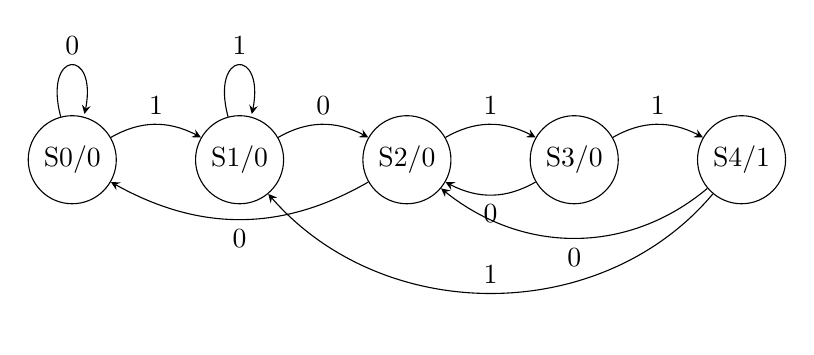
\begin{tikzpicture}[->, >=stealth, node distance=3cm, auto, scale=0.85]
  \node[draw, circle] (S0) at (0,0) {S0/0};
  \node[draw, circle] (S1) at (2.5,0) {S1/0};
  \node[draw, circle] (S2) at (5,0) {S2/0};
  \node[draw, circle] (S3) at (7.5,0) {S3/0};
  \node[draw, circle] (S4) at (10,0) {S4/1};

  \draw (S0) edge[loop above] node{0} (S0);
  \draw (S0) edge[bend left] node{1} (S1);
  \draw (S1) edge[loop above] node{1} (S1);
  \draw (S1) edge[bend left] node{0} (S2);
  \draw (S2) edge[bend left] node{0} (S0);
  \draw (S2) edge[bend left] node{1} (S3);
  \draw (S3) edge[bend left] node{0} (S2);
  \draw (S3) edge[bend left] node{1} (S4);
  \draw (S4) edge[bend left=40] node{0} (S2);
  \draw (S4) edge[bend left=50] node[above]{1} (S1);
\end{tikzpicture}
\end{center}

\textbf{Moore型标注规则：}输出标在状态圈内（状态名/输出值），转移弧上只标输入值。S0-S3输出为0，S4输出为1。

\subsection{状态转移分析}

\begin{itemize}
  \item \textbf{S0}：din=0→S0；din=1→S1
  \item \textbf{S1}：din=0→S2；din=1→S1（"11"的后一个1仍是有效前缀）
  \item \textbf{S2}：din=0→S0；din=1→S3
  \item \textbf{S3}：din=0→S2（"1010"的后缀"10"匹配前缀）；din=1→S4
  \item \textbf{S4}：din=0→S2；din=1→S1（\textbf{可重叠}：末尾1可作为下一组序列起始）
\end{itemize}

\subsection{状态转移表}

\begin{center}
\begin{tabular}{|c|c|c||c|}
\hline
\textbf{当前状态} & \textbf{输入 din} & \textbf{下一状态} & \textbf{输出 y} \\
\hline
S0 & 0 & S0 & 0 \\
S0 & 1 & S1 & 0 \\
S1 & 0 & S2 & 0 \\
S1 & 1 & S1 & 0 \\
S2 & 0 & S0 & 0 \\
S2 & 1 & S3 & 0 \\
S3 & 0 & S2 & 0 \\
S3 & 1 & S4 & 0 \\
S4 & 0 & S2 & 1 \\
S4 & 1 & S1 & 1 \\
\hline
\end{tabular}
\end{center}

\subsection{VHDL实现（两段式，异步高电平复位）}

\begin{lstlisting}[caption={Moore型1011序列检测器（5状态，可重叠）}]
library ieee;
use ieee.std_logic_1164.all;

entity seq1011_moore is
  port(
    clk : in  std_logic;   -- 系统时钟，上升沿有效
    rst : in  std_logic;   -- 异步高电平复位
    din : in  std_logic;   -- 串行数据输入
    y   : out std_logic    -- 检测输出，高电平表示检测到1011
  );
end entity seq1011_moore;

architecture behav of seq1011_moore is
  type state_type is (S0, S1, S2, S3, S4);
  signal curr_state, next_state : state_type;
begin
  -- 第一段：时序逻辑（状态寄存器，时钟+异步复位）
  reg_proc: process(clk, rst)
  begin
    if rst = '1' then
      curr_state <= S0;
    elsif rising_edge(clk) then
      curr_state <= next_state;
    end if;
  end process reg_proc;

  -- 第二段：组合逻辑（状态转移判断）
  comb_proc: process(curr_state, din)
  begin
    case curr_state is
      when S0 =>
        if din = '1' then next_state <= S1;
        else next_state <= S0; end if;
      when S1 =>
        if din = '0' then next_state <= S2;
        else next_state <= S1; end if;
      when S2 =>
        if din = '1' then next_state <= S3;
        else next_state <= S0; end if;
      when S3 =>
        if din = '1' then next_state <= S4;
        else next_state <= S2; end if;
      when S4 =>
        if din = '1' then next_state <= S1;   -- 重叠
        else next_state <= S2; end if;
      when others =>
        next_state <= S0;
    end case;
  end process comb_proc;

  -- Moore型输出：仅由当前状态决定
  y <= '1' when curr_state = S4 else '0';
end architecture behav;
\end{lstlisting}

\section{1101序列检测器（Moore型）}

检测目标：1101。5状态严格Moore，S4为专用输出状态。

状态定义：
\begin{itemize}
  \item S0：初始（匹配0位）\quad S1：已匹配"1"\quad S2：已匹配"11"
  \item S3：已匹配"110"\quad S4：匹配完整序列"1101"，输出y=1
\end{itemize}

\begin{center}
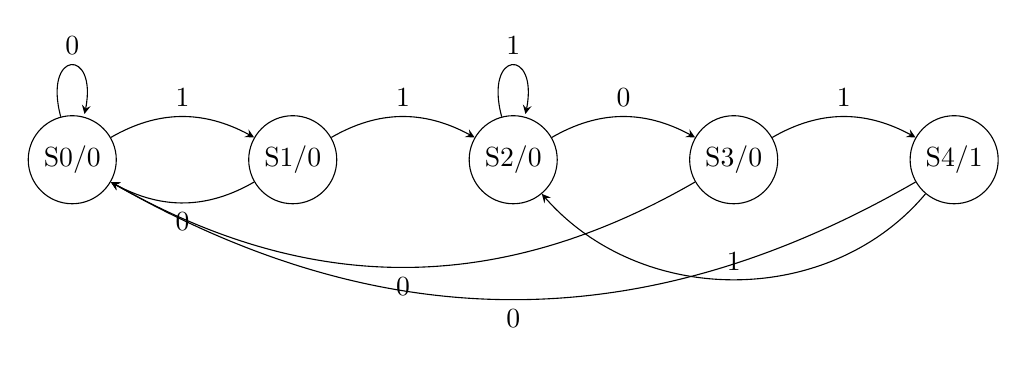
\begin{tikzpicture}[->, >=stealth, node distance=2.8cm, auto]
  \node[draw, circle] (S0) at (0,0) {S0/0};
  \node[draw, circle] (S1) at (2.8,0) {S1/0};
  \node[draw, circle] (S2) at (5.6,0) {S2/0};
  \node[draw, circle] (S3) at (8.4,0) {S3/0};
  \node[draw, circle] (S4) at (11.2,0) {S4/1};

  \draw (S0) edge[loop above] node{0} (S0);
  \draw (S0) edge[bend left] node{1} (S1);
  \draw (S1) edge[bend left] node{0} (S0);
  \draw (S1) edge[bend left] node{1} (S2);
  \draw (S2) edge[loop above] node{1} (S2);
  \draw (S2) edge[bend left] node{0} (S3);
  \draw (S3) edge[bend left] node{0} (S0);
  \draw (S3) edge[bend left] node{1} (S4);
  \draw (S4) edge[bend left=30] node{0} (S0);
  \draw (S4) edge[bend left=50] node[above]{1} (S2);
\end{tikzpicture}
\end{center}

状态转移：S0+1→S1, S1+1→S2, S2+0→S3, S3+1→S4（检测到！）。S4+0→S0, S4+1→S2（重叠：末尾的"1"可开始新序列）。

\section{重叠检测 vs 非重叠检测}

这是\textbf{必考的区别}！

\begin{definition}[重叠检测]
检测到序列后，已匹配的后缀可以用于下一次匹配。

例：输入 ...1011011...（检测1011，重叠）

第一次检测：1 0 \textbf{1 1} 0 1 1 → 在位置4检测到1011
第二次检测：1 0 1 \textbf{1 0 1 1} → 位置4的"11"中的第二个"1"开始新匹配
\end{definition}

\begin{definition}[非重叠检测]
检测到序列后，重新从初始状态开始。

例：输入 ...1011011...（检测1011，非重叠）

第一次检测：1 0 \textbf{1 1} 0 1 1 → 在位置4检测到1011
第二次检测：1 0 1 1 \textbf{0 1 1} ... → 从位置5重新开始（忽略位置4的后缀）
\end{definition}

\textbf{写作VHDL的区别}：

重叠检测：在检测到状态，根据输入决定返回哪个状态（可能有重叠前缀）
非重叠检测：检测到后，直接回到S0/S1（看具体情况）

\section{Moore型 vs Mealy型——考试必考核心对比}

\subsection{两种状态机模型的根本区别}

\begin{keypoint}[Moore vs Mealy的本质]
\textbf{Moore型状态机}：输出\textbf{仅取决于当前状态}。

\textbf{Mealy型状态机}：输出取决于\textbf{当前状态 + 当前输入}。

这个区别看似微小，但导致了两者在\textbf{状态数}、\textbf{输出时序}和\textbf{硬件结构}上的显著差异。
\end{keypoint}

\subsection{Moore型1011序列检测器（5状态）}

\textbf{【状态定义】}严格Moore型使用5个状态，S4为专用输出状态。

\begin{center}
\begin{tabular}{|c|l|c|}\hline
状态 & 含义 & 输出 y \\ \hline
S0 & 未匹配任何有效前缀（初始/复位）& 0 \\
S1 & 已匹配第1位："1" & 0 \\
S2 & 已匹配前2位："10" & 0 \\
S3 & 已匹配前3位："101" & 0 \\
S4 & 匹配完整序列"1011" & \textbf{1} \\ \hline
\end{tabular}
\end{center}

\textbf{【状态转移图】}输出标在状态圈内（Moore型标志）。

\begin{center}
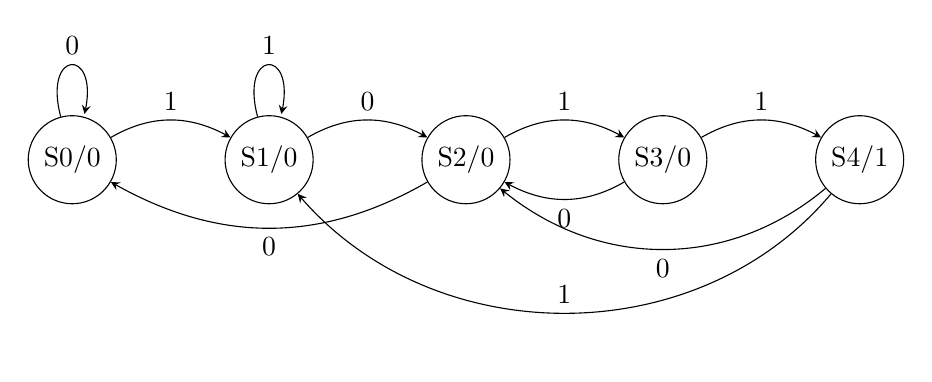
\begin{tikzpicture}[->,>=stealth,node distance=2.5cm,auto]
\node[draw,circle] (S0) at (0,0) {S0/0};
\node[draw,circle] (S1) at (2.5,0) {S1/0};
\node[draw,circle] (S2) at (5,0) {S2/0};
\node[draw,circle] (S3) at (7.5,0) {S3/0};
\node[draw,circle] (S4) at (10,0) {S4/1};
\draw (S0) edge[loop above] node{0} (S0);
\draw (S0) edge[bend left] node{1} (S1);
\draw (S1) edge[loop above] node{1} (S1);
\draw (S1) edge[bend left] node{0} (S2);
\draw (S2) edge[bend left] node{0} (S0);
\draw (S2) edge[bend left] node{1} (S3);
\draw (S3) edge[bend left] node{0} (S2);
\draw (S3) edge[bend left] node{1} (S4);
\draw (S4) edge[bend left=40] node{0} (S2);
\draw (S4) edge[bend left=50] node[above]{1} (S1);
\end{tikzpicture}
\end{center}

\textbf{【输出逻辑】}严格Moore型，$y=1$ 当且仅当 $curr\_state=S4$，与当前输入din无关。进入S4后输出持续整个状态周期（稳定无毛刺）。

\subsection{Mealy型1011序列检测器（4状态）}

\textbf{【状态定义】}Mealy型用4个状态，无专用输出状态，输出在转移弧上。

\begin{center}
\begin{tabular}{|c|l|}\hline
状态 & 含义 \\ \hline
S0 & 未匹配任何有效前缀 \\
S1 & 已匹配第1位："1" \\
S2 & 已匹配前2位："10" \\
S3 & 已匹配前3位："101" \\ \hline
\end{tabular}
\end{center}

\textbf{【状态转移图（标注格式：输入/输出）】}

\begin{center}
\begin{tikzpicture}[->,>=stealth,node distance=3cm,auto]
\node[draw,circle] (S0) at (0,0) {S0};
\node[draw,circle] (S1) at (3,0) {S1};
\node[draw,circle] (S2) at (6,0) {S2};
\node[draw,circle] (S3) at (9,0) {S3};
\draw (S0) edge[loop above] node{0/0} (S0);
\draw (S0) edge[bend left] node{1/0} (S1);
\draw (S1) edge[bend left] node{1/0} (S1);
\draw (S1) edge[bend left] node{0/0} (S2);
\draw (S2) edge[bend left] node{0/0} (S0);
\draw (S2) edge[bend left] node{1/0} (S3);
\draw (S3) edge[bend left=30] node{0/0} (S2);
\draw (S3) edge[bend left=50] node[above]{1/\textbf{1}} (S1);
\end{tikzpicture}
\end{center}

$S3 \xrightarrow{1/1} S1$：输入=1时y=1（检测到1011），去S1（可重叠——末尾1作新序列起始）。

\textbf{【关键对比】}
\begin{itemize}
  \item \textbf{Moore：5状态(S0-S4)}，输出仅取决于当前状态，$y=1$ when $curr\_state=S4$
  \item \textbf{Mealy：4状态(S0-S3)}，无S4，输出在S3+din=1的转移弧上直接产生
  \item Moore输出晚1拍（等状态稳定），Mealy输出与输入同步
\end{itemize}

\subsection{完整对比表}

\begin{center}
\begin{tabular}{|l|c|c|}\hline
\textbf{对比维度} & \textbf{Moore型} & \textbf{Mealy型} \\ \hline
输出决定因素 & 仅当前状态 & 状态 + 输入 \\ \hline
状态数(检测1011) & 5个(S0-S4) & 4个(S0-S3) \\ \hline
输出时序 & 进入S4后输出（晚1拍）& 转移同时输出（同步）\\ \hline
输出持续时间 & 整个S4周期（稳定）& 仅在条件满足时 \\ \hline
对输入毛刺敏感 & 不敏感（只看状态）& 敏感（输入参与输出）\\ \hline
状态图标注 & 状态圈内"状态/输出"& 转移弧上"输入/输出"\\ \hline
综合结果 & 3FF+输出逻辑 & 2FF+次态/输出组合逻辑 \\ \hline
考试推荐 & 更安全稳定，优先使用 & 更紧凑，按题目要求 \\ \hline
\end{tabular}
\end{center}

\subsection{VHDL实现对比（两段式，异步高电平复位）}

\textbf{【Moore型——5状态，可重叠】}

\begin{lstlisting}[caption={Moore型1011序列检测器}]
library ieee;
use ieee.std_logic_1164.all;

entity seq1011_moore is
  port(
    clk : in  std_logic;
    rst : in  std_logic;   -- 异步高电平复位
    din : in  std_logic;
    y   : out std_logic
  );
end entity seq1011_moore;

architecture behav of seq1011_moore is
  type state_type is (S0, S1, S2, S3, S4);
  signal curr_state, next_state : state_type;
begin
  -- 第一段：时序逻辑（状态寄存器）
  reg_proc: process(clk, rst)
  begin
    if rst = '1' then curr_state <= S0;
    elsif rising_edge(clk) then curr_state <= next_state;
    end if;
  end process reg_proc;

  -- 第二段：组合逻辑（状态转移）
  comb_proc: process(curr_state, din)
  begin
    case curr_state is
      when S0 =>
        if din = '1' then next_state <= S1;
        else next_state <= S0; end if;
      when S1 =>
        if din = '0' then next_state <= S2;
        else next_state <= S1; end if;
      when S2 =>
        if din = '1' then next_state <= S3;
        else next_state <= S0; end if;
      when S3 =>
        if din = '1' then next_state <= S4;
        else next_state <= S2; end if;
      when S4 =>
        if din = '1' then next_state <= S1;   -- 重叠
        else next_state <= S2; end if;
      when others => next_state <= S0;
    end case;
  end process comb_proc;

  -- Moore输出：仅由当前状态决定
  y <= '1' when curr_state = S4 else '0';
end architecture behav;
\end{lstlisting}

\textbf{【Mealy型——4状态，可重叠，默认赋值】}

\begin{lstlisting}[caption={Mealy型1011序列检测器}]
library ieee;
use ieee.std_logic_1164.all;

entity seq1011_mealy is
  port(
    clk : in  std_logic;
    rst : in  std_logic;   -- 异步高电平复位
    din : in  std_logic;
    y   : out std_logic
  );
end entity seq1011_mealy;

architecture behav of seq1011_mealy is
  type state_type is (S0, S1, S2, S3);
  signal curr_state, next_state : state_type;
begin
  -- 第一段：时序逻辑（状态寄存器）
  reg_proc: process(clk, rst)
  begin
    if rst = '1' then curr_state <= S0;
    elsif rising_edge(clk) then curr_state <= next_state;
    end if;
  end process reg_proc;

  -- 第二段：组合逻辑（状态转移 + Mealy输出）
  comb_proc: process(curr_state, din)
  begin
    -- 默认赋值，避免组合逻辑锁存
    next_state <= S0;
    y <= '0';

    case curr_state is
      when S0 =>
        if din = '1' then next_state <= S1;
        else next_state <= S0; end if;
      when S1 =>
        if din = '0' then next_state <= S2;
        else next_state <= S1; end if;
      when S2 =>
        if din = '1' then next_state <= S3;
        else next_state <= S0; end if;
      when S3 =>
        if din = '1' then
          next_state <= S1;
          y <= '1';  -- 检测到1011，输出有效（重叠）
        else
          next_state <= S2;
        end if;
      when others => next_state <= S0;
    end case;
  end process comb_proc;
end architecture behav;
\end{lstlisting}

\textbf{【关键代码差异】}
\begin{itemize}
  \item \textbf{Moore}：5状态，输出在进程外：\texttt{y <= '1' when curr\_state = S4 else '0';}
  \item \textbf{Mealy}：4状态，输出在comb\_proc内：\texttt{y <= '1';}（默认为0，检测到时置1）
  \item \textbf{默认赋值}（Mealy必须）：\texttt{next\_state <= S0; y <= '0';} 写在case之前，避免锁存
  \item \textbf{可重叠/非重叠切换}：改S4/S3的din=1跳转——回S0=非重叠，回S1=重叠
\end{itemize}

\subsection{输出时序对比}

\textbf{【Moore型输出晚1拍】}

\begin{center}
\begin{tabular}{|c|c|c|c|c||c|c|}\hline
时钟拍 & 1 & 2 & 3 & 4 & 5 \\ \hline
输入din & 1 & 0 & 1 & 1 & 0 \\ \hline
Moore curr\_state & S1 & S2 & S3 & S4 & S1 \\ \hline
Moore输出y & 0 & 0 & 0 & \textbf{1}（第4拍！）& 0 \\ \hline
\hline
Mealy curr\_state & S1 & S2 & S3 & S1 & S2 \\ \hline
Mealy输出y & 0 & 0 & 0 & \textbf{1}（第4拍！）& 0 \\ \hline
\end{tabular}
\end{center}

注：严格5状态Moore进入S4即输出$y=1$，在第4拍（与Mealy同拍）输出。Moore输出仅取决于当前状态是否为S4，与输入din无关，这是Moore型与Mealy型的根本区别。

\subsection{考试如何选择}

\begin{examtip}[Moore vs Mealy考试策略]
\begin{enumerate}
  \item \textbf{默认选Moore型（5状态）}：状态图更清晰，输出稳定，符合教材规范
  \item \textbf{题目明确要求Mealy型时才用Mealy（4状态）}
  \item \textbf{状态图标注规范}：
  \begin{itemize}
    \item Moore：状态圈内写"状态名/输出值"（如S0/0, S4/1）
    \item Mealy：转移弧上写"输入值/输出值"（如1/1）
  \end{itemize}
  \item \textbf{VHDL必须用两段式}：时序reg\_proc + 组合comb\_proc
  \item \textbf{Mealy必须有默认赋值}：避免组合逻辑锁存
\end{enumerate}
\end{examtip}

\subsection{硬件综合结果对比}

\begin{center}
\begin{tabular}{|l|c|c|}
\hline
\textbf{硬件模块} & \textbf{Moore型} & \textbf{Mealy型} \\
\hline
状态寄存器 & 3个D触发器（编码5状态）& 2个D触发器（编码4状态）\\
次态逻辑 & 组合电路（当前状态+din → 下一状态）& 组合电路（当前状态+din → 下一状态）\\
输出逻辑 & 独立组合电路（仅读当前状态）& 合并于次态逻辑中（读当前状态+din）\\
输出信号y & S4时y=1，与din无关 & S3且din=1时y=1，随转移产生\\
\hline
关键路径延迟 & 寄存器延迟 + 次态逻辑延迟 & 寄存器延迟 + 次态/输出组合延迟 \\
输出毛刺风险 & 低（仅状态变化时输出才变）& 较高（din直接参与输出）\\
\hline
\end{tabular}
\end{center}

\textbf{结论}：Moore型输出稳定、无毛刺，适合对时序要求严格的场合。Mealy型状态少、响应快，但输出可能受输入毛刺影响。考试中优先使用Moore型。

\section{考试常见变式}

\begin{enumerate}
  \item \textbf{变式1：检测1011（重叠）}

  检测后在S3状态，输入1→检测到，同时此1可作为新序列的第一个1，因此去S1（不是S0）。

  \item \textbf{变式2：检测0101}

  状态：S0（初始）→S1（匹配"0"）→S2（匹配"01"）→S3（匹配"010"）。S3+输入1=检测到。

  \item \textbf{变式3：检测1111}

  4个连续的1。状态：S0→S1（1个1）→S2（2个1）→S3（3个1）。S3+输入1=检测到（重叠：保持S3）。

  \item \textbf{变式4：同时检测多个序列}

  如同时检测1011和1101。需要合并两个状态机。

  \item \textbf{变式5：Mealy型 vs Moore型检测器}

  Mealy：输出取决于状态+输入（输出可以早一拍）
  Moore：输出仅取决于状态（输出晚一拍，但更稳定）

  考试通常要求Moore型。
\end{enumerate}

\section{Testbench}

\begin{lstlisting}[caption={Moore型1011序列检测器Testbench（异步高电平复位）}]
library ieee;
use ieee.std_logic_1164.all;

entity seq1011_moore_tb is
end seq1011_moore_tb;

architecture test of seq1011_moore_tb is
  signal clk, rst, din, y : std_logic;
  constant T : time := 20 ns;

  component seq1011_moore is
    port(clk, rst, din : in std_logic; y : out std_logic);
  end component;
begin
  uut: seq1011_moore port map(clk, rst, din, y);

  clk <= not clk after T/2;

  stimulus: process
  begin
    rst <= '1'; wait for 30 ns;  -- 异步高电平复位
    rst <= '0'; wait for 5 ns;

    -- 输入序列：1 0 1 1 0 1 0 1 1（可重叠验证）
    din <= '1'; wait for T;  -- S0→S1
    din <= '0'; wait for T;  -- S1→S2
    din <= '1'; wait for T;  -- S2→S3
    din <= '1'; wait for T;  -- S3→S4, y=1（检测到！）
    din <= '0'; wait for T;
    din <= '1'; wait for T;
    din <= '0'; wait for T;
    din <= '1'; wait for T;
    din <= '1'; wait for T;  -- 第9拍再次检测到！
    wait;
  end process;
end test;
\end{lstlisting}

\begin{examtip}[序列检测器秒杀法]
\textbf{第一步：确定状态}
状态 = 已匹配的序列前缀（每个状态代表匹配了序列的前几位）

\textbf{第二步：画状态图}
对每个状态，考虑输入0和输入1分别去哪里

\textbf{第三步：写状态转移表}

\textbf{第四步：写VHDL}
\begin{itemize}
  \item type定义状态枚举
  \item case语句处理每个状态
  \item 检测到条件：在倒数第二个状态 + 最后一个匹配位
\end{itemize}

\textbf{关键技巧}：状态S3下输入1→检测到。但去哪？
\begin{itemize}
  \item 重叠检测：分析后几位能否作为新前缀→S1（"1011"最后的"1"可以是新序列的第一个"1"）
  \item 非重叠检测：直接回S0
\end{itemize}
\end{examtip}

\section{状态机的其他应用——不止序列检测器}

序列检测器是状态机最经典的应用，但状态机的应用远不止于此。实际上，前面学过的很多电路本质上都是状态机。

\subsection{计数器 = 状态机}

\textbf{用状态机的眼光重新看模6计数器：}

\begin{center}
\begin{tabular}{|c|c|c|}
\hline
\textbf{状态机要素} & \textbf{模6计数器对应} & \textbf{硬件实现} \\
\hline
当前状态 & cnt[2:0]（3位D触发器）& 3个DFF \\
次态逻辑 & $cnt_{next} = cnt + 1$（若$cnt=5$则归0）& 加法器+比较器 \\
输出逻辑 & count = cnt, carry = 1 when cnt=5 & 连线+比较器 \\
\hline
\end{tabular}
\end{center}

\textbf{状态转移图（模6计数器）：}

\begin{center}
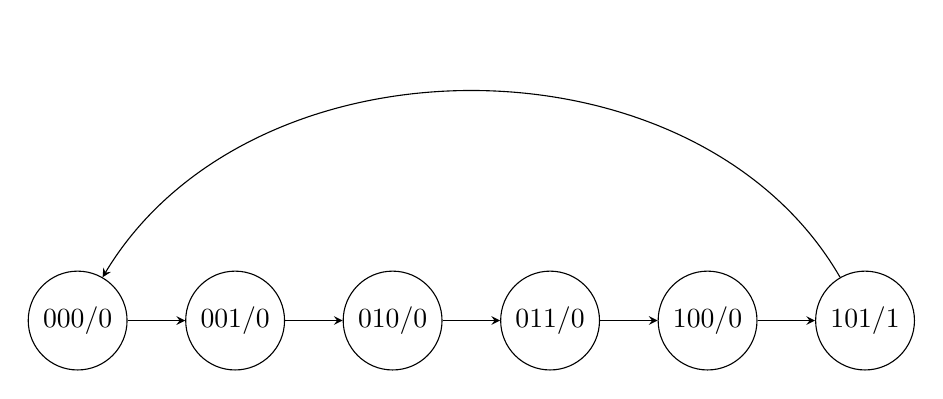
\begin{tikzpicture}[->,>=stealth,node distance=2cm,auto]
\node[draw,circle] (s0) at (0,0) {000/0};
\node[draw,circle] (s1) at (2,0) {001/0};
\node[draw,circle] (s2) at (4,0) {010/0};
\node[draw,circle] (s3) at (6,0) {011/0};
\node[draw,circle] (s4) at (8,0) {100/0};
\node[draw,circle] (s5) at (10,0) {101/1};
\draw (s0) -- (s1); \draw (s1) -- (s2); \draw (s2) -- (s3);
\draw (s3) -- (s4); \draw (s4) -- (s5);
\draw (s5) edge[bend right=60] (s0);
\end{tikzpicture}
\end{center}
（状态标注格式：计数值/carry输出）

\textbf{用直观状态机写法重写模6计数器：}

\begin{lstlisting}[caption={模6计数器——每个状态一行，输出和下一拍一起写}]
architecture Behavioral of counter_mod6_fsm is
  type state is (s0,s1,s2,s3,s4,s5);
  signal present_state, next_state: state;
begin
  process(rst, clk)
  begin
    if rst='0' then present_state <= s0;
    elsif clk'event and clk='1' then
      present_state <= next_state;
    end if;
  end process;

  COM: process(present_state)
  begin
    case present_state is
      when s0 => count<="000"; carry<='0'; next_state<=s1;
      when s1 => count<="001"; carry<='0'; next_state<=s2;
      when s2 => count<="010"; carry<='0'; next_state<=s3;
      when s3 => count<="011"; carry<='0'; next_state<=s4;
      when s4 => count<="100"; carry<='0'; next_state<=s5;
      when s5 => count<="101"; carry<='1'; next_state<=s0;
      when others => count<="000"; carry<='0'; next_state<=s0;
    end case;
  end process COM;
end Behavioral;
\end{lstlisting}

\textbf{对比：}上面用的是\textbf{枚举6个状态}的写法（6个when分支），下面是用加法器+清零的写法：

\begin{lstlisting}[caption={模6计数器——传统写法（等价但更简洁）}]
  if cnt = 5 then cnt <= 0; else cnt <= cnt + 1; end if;
\end{lstlisting}

两段代码\textbf{完全等价}——综合出来的硬件一模一样。但枚举写法让你看清：计数器就是一个6状态的循环状态机。

\textbf{拓展练习：用状态机实现模5计数器}

将上面模6的方法直接套用到模5：5个状态s0-s4。

\begin{lstlisting}[caption={模5计数器——直观状态机写法}]
type state is (s0,s1,s2,s3,s4);
signal present_state, next_state: state;
...
COM: process(present_state)
begin
  case present_state is
    when s0 => count<="000"; next_state<=s1;
    when s1 => count<="001"; next_state<=s2;
    when s2 => count<="010"; next_state<=s3;
    when s3 => count<="011"; next_state<=s4;
    when s4 => count<="100"; next_state<=s0;
    when others => count<="000"; next_state<=s0;
  end case;
end process COM;
\end{lstlisting}

\textbf{任意模N计数器都可以这样写——N个状态，N个when分支。}每个分支写清楚当前状态输出什么值、下一拍去哪里。模12=12行，模24=24行，以此类推。

\subsection{分频器 = 状态机}

分频器的本质：一个状态在$M$个状态间循环，输出在特定状态翻转。

\textbf{例题：12分频器（占空比50\%）。}$M=12$，需要12个状态。前6个状态输出0，后6个状态输出1。

\textbf{状态转移图（12状态循环）：}
\begin{center}
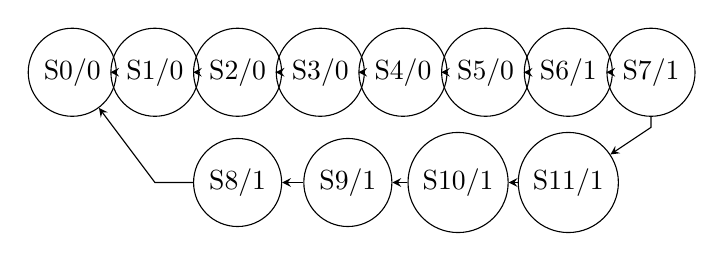
\begin{tikzpicture}[->,>=stealth,node distance=1.3cm,auto,scale=0.7]
\node[draw,circle] (s0) at (0,0) {S0/0};
\node[draw,circle] (s1) at (1.5,0) {S1/0};
\node[draw,circle] (s2) at (3,0) {S2/0};
\node[draw,circle] (s3) at (4.5,0) {S3/0};
\node[draw,circle] (s4) at (6,0) {S4/0};
\node[draw,circle] (s5) at (7.5,0) {S5/0};
\node[draw,circle] (s6) at (9,0) {S6/1};
\node[draw,circle] (s7) at (10.5,0) {S7/1};
\node[draw,circle] (s8) at (3,-2) {S8/1};
\node[draw,circle] (s9) at (5,-2) {S9/1};
\node[draw,circle] (sa) at (7,-2) {S10/1};
\node[draw,circle] (sb) at (9,-2) {S11/1};
\draw (s0)--(s1); \draw (s1)--(s2); \draw (s2)--(s3); \draw (s3)--(s4);
\draw (s4)--(s5); \draw (s5)--(s6); \draw (s6)--(s7);
\draw (s7) -- (10.5,-1) -- (sb);
\draw (sb)--(sa); \draw (sa)--(s9); \draw (s9)--(s8);
\draw (s8) -- (1.5,-2) -- (s0);
\end{tikzpicture}
\end{center}
（S0-S5输出0，S6-S11输出1，12个状态循环。6拍低+6拍高=50\%占空比。）

\textbf{VHDL——直观状态机写法：}
\begin{lstlisting}[caption={12分频器——每个状态一行，输出和转移一起写}]
architecture Behavioral of div12_fsm is
  type state is (s0,s1,s2,s3,s4,s5,s6,s7,s8,s9,s10,s11);
  signal present_state, next_state: state;
begin
  process(rst, clk)
  begin
    if rst='0' then present_state <= s0;
    elsif clk'event and clk='1' then
      present_state <= next_state;
    end if;
  end process;

  COM: process(present_state)
  begin
    case present_state is
      when s0  => clk_out<='0'; next_state<=s1;
      when s1  => clk_out<='0'; next_state<=s2;
      when s2  => clk_out<='0'; next_state<=s3;
      when s3  => clk_out<='0'; next_state<=s4;
      when s4  => clk_out<='0'; next_state<=s5;
      when s5  => clk_out<='0'; next_state<=s6;
      when s6  => clk_out<='1'; next_state<=s7;
      when s7  => clk_out<='1'; next_state<=s8;
      when s8  => clk_out<='1'; next_state<=s9;
      when s9  => clk_out<='1'; next_state<=s10;
      when s10 => clk_out<='1'; next_state<=s11;
      when s11 => clk_out<='1'; next_state<=s0;
      when others => clk_out<='0'; next_state<=s0;
    end case;
  end process COM;
end Behavioral;
\end{lstlisting}

\textbf{和传统计数器写法对比：}
\begin{lstlisting}[caption={传统写法（模12计数器+比较）}]
if cnt=11 then cnt<=0; else cnt<=cnt+1; end if;
clk_out <= '0' when cnt < 6 else '1';
\end{lstlisting}

同样等价！状态机12状态枚举写法更直观——你看状态图就知道输出波形是什么。计数器写法更紧凑——4位计数器+比较器搞定。\textbf{考试中两种写法都正确，状态机写法更容易画状态转移图拿步骤分。}

\subsection{移位寄存器 = 状态机}

移位寄存器的"状态"就是N个D触发器的内容——一个N位向量，总共$2^N$种可能。次态函数非常简单：$Q_{next} = \{si, Q[N-1:1]\}$（右移）或$\{Q[N-2:0], si\}$（左移）。

\textbf{本质上它是状态机，但次态逻辑太简单了——一行拼接就表达完毕，不需要case枚举。}

\textbf{移位寄存器是状态机——但你不会用case去写它。}

4位移位寄存器有$2^4=16$个状态。\textbf{理论上}可以枚举16个状态用case写——比如状态"0000"输入1→下一拍"1000"；状态"1000"输入0→下一拍"0100"...以此类推，16个状态×2种输入=32个when分支。

\textbf{但没人会这样写}——太蠢了。一行\texttt{reg <= si \& reg(3 downto 1)}就搞定的事情，写32行case毫无意义。

\textbf{这说明一个重要区别：}
\begin{itemize}
  \item 有些电路的次态逻辑\textbf{有简洁的数学表达}（移位=拼接、计数=+1）→ 不需要枚举状态
  \item 有些电路没有（序列检测的前缀匹配、售货机的金额累计）→ \textbf{必须}枚举状态
\end{itemize}

\textbf{什么时候必须用显式状态机？}次态逻辑没有简洁公式时。序列检测器检测1011——你没法用一个数学表达式描述"已匹配101时输入1→检测到"，所以必须枚举S0/S1/S2/S3四个状态。计数器和移位寄存器的次态有简洁公式（+1和拼接），用传统写法即可。

\textbf{环形计数器和Johnson计数器}是移位寄存器的特例：反馈线不同，同样不需要显式状态机。

\subsection{序列发生器 = 状态机}

序列发生器是\textbf{无外部输入的状态机}— 没有din，次态只取决于当前状态。以序列00011101为例：

\textbf{状态转移图（8状态，无输入）：}

\begin{center}
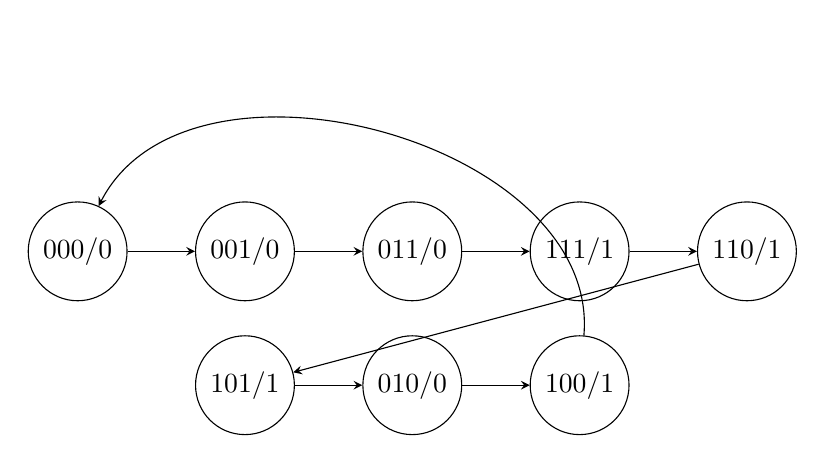
\begin{tikzpicture}[->,>=stealth,node distance=1.8cm,auto,scale=0.85]
\node[draw,circle] (s0) at (0,0) {000/0};
\node[draw,circle] (s1) at (2.5,0) {001/0};
\node[draw,circle] (s2) at (5,0) {011/0};
\node[draw,circle] (s3) at (7.5,0) {111/1};
\node[draw,circle] (s4) at (10,0) {110/1};
\node[draw,circle] (s5) at (2.5,-2) {101/1};
\node[draw,circle] (s6) at (5,-2) {010/0};
\node[draw,circle] (s7) at (7.5,-2) {100/1};
\draw (s0) -- (s1); \draw (s1) -- (s2); \draw (s2) -- (s3);
\draw (s3) -- (s4); \draw (s4) -- (s5); \draw (s5) -- (s6);
\draw (s6) -- (s7); \draw (s7) edge[bend right=80] (s0);
\end{tikzpicture}
\end{center}
（状态标注格式：Q/输出值。转移弧上无标注——因为没有外部输入。）

\textbf{注意和序列检测器的对比：}
\begin{itemize}
  \item 检测器弧上有输入值(0/1)，因为去哪取决于din
  \item 发生器弧上没有输入，因为去哪是确定的（CASE表写死了）
\end{itemize}

\textbf{用状态机写法实现：}

\begin{lstlisting}[caption={序列发生器00011101——直观状态机写法}]
architecture Behavioral of seqgen_fsm is
  type state is (s0,s1,s2,s3,s4,s5,s6,s7);
  signal present_state, next_state: state;
begin
  -- 状态寄存器
  process(rst, clk)
  begin
    if rst='0' then present_state <= s0;
    elsif clk'event and clk='1' then
      present_state <= next_state;
    end if;
  end process;

  -- 次态逻辑 + 输出（每个状态一行：输出什么 + 下一拍去哪）
  COM: process(present_state)
  begin
    case present_state is
      when s0 => q <= '0'; next_state <= s1;
      when s1 => q <= '0'; next_state <= s2;
      when s2 => q <= '0'; next_state <= s3;
      when s3 => q <= '1'; next_state <= s4;
      when s4 => q <= '1'; next_state <= s5;
      when s5 => q <= '1'; next_state <= s6;
      when s6 => q <= '0'; next_state <= s7;
      when s7 => q <= '1'; next_state <= s0;
      when others => q <= '0'; next_state <= s0;
    end case;
  end process COM;
end Behavioral;
\end{lstlisting}

\textbf{这种写法的好处：}每个状态一行——\texttt{when s3 => q <= '1'; next\_state <= s4;} → 状态s3输出1，下一拍去s4。8个状态8行，序列00011101直接写在代码里，一目了然。和状态转移图完全对应——图上每个圈写什么，代码里每个when就写什么。

\textbf{和移位寄存器+CASE表写法对比：}两者功能完全相同。状态机枚举写法更直观（8个状态看得清清楚楚），查表写法更紧凑（不需要枚举状态类型）。

\subsection{统一视角}

\begin{center}
\begin{tikzpicture}[>=stealth]
\node[draw,minimum width=3cm,minimum height=1cm] (reg) at (0,0) {状态寄存器(D触发器)};
\node[draw,minimum width=3cm,minimum height=1.2cm] (nsl) at (5,0) {次态逻辑};
\node[draw,minimum width=3cm,minimum height=1cm] (ol) at (5,-2) {输出逻辑};
\draw[->] (reg) -- (nsl) node[midway,above]{当前状态};
\draw[->] (nsl.east) -- ++(1,0) |- (reg.north) node[near end,right]{下一状态};
\draw[->] (reg.east) -- ++(0.5,0) |- (ol.west);
\draw[->] (ol.east) -- ++(1.5,0) node[right]{输出};
\node at (2.5,-3.5) {所有同步时序电路都遵循这个结构};
\end{tikzpicture}
\end{center}

\begin{center}
\begin{tabular}{|l|c|c|c|}
\hline
\textbf{电路} & \textbf{次态逻辑} & \textbf{输出逻辑} & \textbf{输入} \\
\hline
计数器 & $+1$ 加法器 & 计数值/进位 & 无（或en/load）\\
移位寄存器 & 移位拼接 & 并行/串行数据 & si/din \\
序列发生器 & CASE查表 & Q最高位 & 无 \\
序列检测器 & 前缀匹配判断 & detected信号 & din串行输入 \\
\hline
\end{tabular}
\end{center}

\textbf{核心结论：}

\begin{center}
\begin{tabular}{|l|c|c|}
\hline
\textbf{电路} & \textbf{次态逻辑} & \textbf{需要显式状态机？} \\
\hline
计数器 & $cnt+1$（有简洁数学公式）& 不需要，一行cnt<=cnt+1即可 \\
移位寄存器 & 拼接运算（有简洁公式）& 不需要，一行reg<=si\&reg即可 \\
序列发生器 & CASE查表/枚举 & 可以（枚举更直观）\\
序列检测器 & 前缀匹配判断 & \textbf{必须}——没有简洁公式 \\
\hline
\end{tabular}
\end{center}

\textbf{什么时候用显式状态机：次态逻辑没有简洁数学表达式的时候。}计数器+1、移位拼接——一行代码搞定。序列检测的前缀匹配、售货机的金额累计——必须老老实实画状态图、写case枚举。\textbf{不是所有电路都要写成状态机，但所有电路都可以用状态机来理解。}

\section{变式详解}
\chapter{序列检测器——全部变式详解}

\section{变式1：检测1011（重叠 vs 非重叠）}

\begin{detailbox}[完整教学]
\textbf{【核心区别】}S3+输入1→检测到！
\begin{itemize}
  \item \textbf{非重叠}→回S0（重新开始）
  \item \textbf{重叠}→去S1（最后的"1"作为新序列的第一个"1"）
\end{itemize}

\textbf{【重叠检测版本——完整VHDL（Moore型，5状态）】}
\begin{lstlisting}[caption={1011序列检测器——Moore型可重叠}]
library ieee;
use ieee.std_logic_1164.all;

entity seq1011_moore is
  port(
    clk : in  std_logic;
    rst : in  std_logic;   -- 异步高电平复位
    din : in  std_logic;
    y   : out std_logic
  );
end entity seq1011_moore;

architecture behav of seq1011_moore is
  type state_type is (S0, S1, S2, S3, S4);
  signal curr_state, next_state : state_type;
begin
  reg_proc: process(clk, rst)
  begin
    if rst = '1' then curr_state <= S0;
    elsif rising_edge(clk) then curr_state <= next_state;
    end if;
  end process reg_proc;

  comb_proc: process(curr_state, din)
  begin
    case curr_state is
      when S0 =>
        if din = '1' then next_state <= S1;
        else next_state <= S0; end if;
      when S1 =>
        if din = '0' then next_state <= S2;
        else next_state <= S1; end if;
      when S2 =>
        if din = '1' then next_state <= S3;
        else next_state <= S0; end if;
      when S3 =>
        if din = '1' then next_state <= S4;
        else next_state <= S2; end if;
      when S4 =>
        if din = '1' then next_state <= S1;   -- 重叠！末尾1→新序列起始
        else next_state <= S2; end if;
      when others => next_state <= S0;
    end case;
  end process comb_proc;

  y <= '1' when curr_state = S4 else '0';
end architecture behav;
\end{lstlisting}

\textbf{【考试判断】}看S4状态的din=1跳转目标。S4+1→S0=非重叠，S4+1→S1=可重叠。
\end{detailbox}


\section{变式2：检测1101}

\begin{detailbox}[完整教学]
\textbf{【状态】}S0→S1→S2→S3→(输入1=检测到)
\textbf{【重叠处理】}S3+1→检测到→去S2（"1101"中后两位"11"匹配"11"前缀）
\textbf{【关键】}S2+1→S2（"111"中后两个"11"为有效前缀）。

\begin{lstlisting}[caption={1101序列检测器——Moore型可重叠（5状态）}]
library ieee;
use ieee.std_logic_1164.all;

entity seq1101_moore is
  port(
    clk : in  std_logic;
    rst : in  std_logic;
    din : in  std_logic;
    y   : out std_logic
  );
end entity seq1101_moore;

architecture behav of seq1101_moore is
  type state_type is (S0, S1, S2, S3, S4);
  signal curr_state, next_state : state_type;
begin
  reg_proc: process(clk, rst)
  begin
    if rst = '1' then curr_state <= S0;
    elsif rising_edge(clk) then curr_state <= next_state;
    end if;
  end process reg_proc;

  comb_proc: process(curr_state, din)
  begin
    case curr_state is
      when S0 =>
        if din = '1' then next_state <= S1;
        else next_state <= S0; end if;
      when S1 =>
        if din = '0' then next_state <= S0;
        else next_state <= S2; end if;
      when S2 =>
        if din = '0' then next_state <= S3;
        else next_state <= S2; end if;   -- din=1保持S2
      when S3 =>
        if din = '1' then next_state <= S4;
        else next_state <= S0; end if;
      when S4 =>
        if din = '1' then next_state <= S2;   -- 重叠
        else next_state <= S0; end if;
      when others => next_state <= S0;
    end case;
  end process comb_proc;

  -- Moore输出：仅取决于状态
  y <= '1' when curr_state = S4 else '0';
end architecture behav;
\end{lstlisting}
\end{detailbox}


\section{变式3：检测1111（连续4个1）}

\begin{detailbox}[完整教学]
\textbf{【状态】}S0→S1(1个1)→S2(2个1)→S3(3个1)→(第4个1→检测)
\textbf{【特点】}任意时刻输入0→回S0（连续中断）。
\textbf{【重叠】}S3+1→S3（"1111"后3个"111"为有效前缀）。

\begin{lstlisting}[caption={1111序列检测器——Moore型可重叠（5状态）}]
library ieee;
use ieee.std_logic_1164.all;

entity seq1111_moore is
  port(
    clk : in  std_logic;
    rst : in  std_logic;
    din : in  std_logic;
    y   : out std_logic
  );
end entity seq1111_moore;

architecture behav of seq1111_moore is
  type state_type is (S0, S1, S2, S3, S4);
  signal curr_state, next_state : state_type;
begin
  reg_proc: process(clk, rst)
  begin
    if rst = '1' then curr_state <= S0;
    elsif rising_edge(clk) then curr_state <= next_state;
    end if;
  end process reg_proc;

  comb_proc: process(curr_state, din)
  begin
    case curr_state is
      when S0 =>
        if din = '1' then next_state <= S1;
        else next_state <= S0; end if;
      when S1 =>
        if din = '1' then next_state <= S2;
        else next_state <= S0; end if;
      when S2 =>
        if din = '1' then next_state <= S3;
        else next_state <= S0; end if;
      when S3 =>
        if din = '1' then next_state <= S4;
        else next_state <= S0; end if;
      when S4 =>
        if din = '1' then next_state <= S4;   -- 重叠！保持S4
        else next_state <= S0; end if;
      when others => next_state <= S0;
    end case;
  end process comb_proc;

  y <= '1' when curr_state = S4 else '0';
end architecture behav;
\end{lstlisting}
\end{detailbox}


\section{变式4：检测0101}

\begin{detailbox}[完整教学]
\textbf{【状态】}检测0101（4位序列），状态按S0-S3顺序命名，每个状态含义取决于目标序列：
\begin{itemize}
  \item S0：初始（匹配0位）
  \item S1：已匹配"0"（序列第一位）
  \item S2：已匹配"01"（序列前两位）
  \item S3：已匹配"010"（序列前三位，等待最后一位1）
\end{itemize}
\textbf{【注意】}S3+1→检测到；S3+0→S1（重叠："0100"最后的"0"可作为新序列第一个"0"）。

\begin{lstlisting}[caption={0101序列检测器——Moore型可重叠（5状态）}]
library ieee;
use ieee.std_logic_1164.all;

entity seq0101_moore is
  port(
    clk : in  std_logic;
    rst : in  std_logic;
    din : in  std_logic;
    y   : out std_logic
  );
end entity seq0101_moore;

architecture behav of seq0101_moore is
  type state_type is (S0, S1, S2, S3, S4);
  signal curr_state, next_state : state_type;
begin
  reg_proc: process(clk, rst)
  begin
    if rst = '1' then curr_state <= S0;
    elsif rising_edge(clk) then curr_state <= next_state;
    end if;
  end process reg_proc;

  comb_proc: process(curr_state, din)
  begin
    case curr_state is
      when S0 =>
        if din = '0' then next_state <= S1;
        else next_state <= S0; end if;
      when S1 =>
        if din = '1' then next_state <= S2;   -- "01"
        else next_state <= S1; end if;         -- "00"保持
      when S2 =>
        if din = '0' then next_state <= S3;   -- "010"
        else next_state <= S0; end if;
      when S3 =>
        if din = '1' then next_state <= S4;   -- "0101"
        else next_state <= S1; end if;         -- "0100"→S1
      when S4 =>
        if din = '0' then next_state <= S1;   -- 重叠
        else next_state <= S0; end if;
      when others => next_state <= S0;
    end case;
  end process comb_proc;

  y <= '1' when curr_state = S4 else '0';
end architecture behav;
\end{lstlisting}
\end{detailbox}


\section{变式5：用移位寄存器+比较器替代状态机}

\begin{detailbox}[完整教学]
\textbf{【方案】}移位寄存器存最近N位→与目标序列比较。
\textbf{【完整VHDL】}
\begin{lstlisting}[caption={移位寄存器+比较器实现1011序列检测}]
library ieee;
use ieee.std_logic_1164.all;

entity seq_detector_shift is
  port(
    clk : in  std_logic;
    rst : in  std_logic;
    din : in  std_logic;
    y   : out std_logic
  );
end seq_detector_shift;

architecture behavioral of seq_detector_shift is
  signal reg : std_logic_vector(3 downto 0);
begin
  process(clk, rst)
  begin
    if rst = '1' then
      reg <= (others => '0');
    elsif rising_edge(clk) then
      reg <= din & reg(3 downto 1);
    end if;
  end process;

  y <= '1' when reg = "1011" else '0';
end behavioral;
\end{lstlisting}
\textbf{【优点】}代码极简。不需推导状态转移。
\textbf{【注意】}自动实现重叠检测。
\textbf{【考试适用】}除非题目明确要求"用状态机设计"，否则移位寄存器方案是最佳选择。
\end{detailbox}


% =============================================================
%  第九部分：VHDL专题
% =============================================================
\part{VHDL硬件综合专题}

\chapter{VHDL硬件综合专题}

\section{学习目标}

不是学VHDL语法。而是理解：

\begin{center}
\fbox{%
\begin{minipage}{0.85\textwidth}
\textbf{你写的每一行VHDL，最终在FPGA中变成了什么硬件？}
\end{minipage}%
}
\end{center}

\section{if-else 综合成什么}

\begin{lstlisting}[caption={if-else示例}]
 if sel = '1' then
  y <= a;
else
  y <= b;
end if;
\end{lstlisting}

\textbf{综合结果：MUX（数据选择器）}

\begin{center}
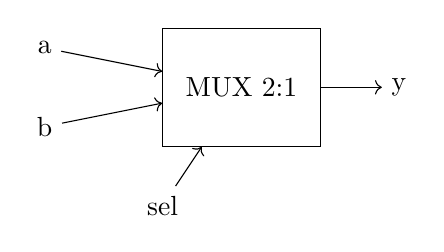
\begin{tikzpicture}
  \node[draw, minimum width=2cm, minimum height=1.5cm] (mux) at (0,0) {MUX 2:1};
  \node (a) at (-2.5,0.5) {a};
  \node (b) at (-2.5,-0.5) {b};
  \node (sel) at (-1,-1.5) {sel};
  \node (y) at (2,0) {y};
  \draw[->] (a) -- (mux);
  \draw[->] (b) -- (mux);
  \draw[->] (sel) -- (mux);
  \draw[->] (mux) -- (y);
\end{tikzpicture}
\end{center}

\subsection{if-else级联}

\begin{lstlisting}
 if sel = "00" then
  y <= d0;
elsif sel = "01" then
  y <= d1;
elsif sel = "10" then
  y <= d2;
else
  y <= d3;
end if;
\end{lstlisting}

\textbf{综合结果：优先级编码的选择器（级联MUX）}。sel=11优先级最低（在最后的else中），综合工具可能优化为并行MUX。

\begin{keypoint}[if-else与硬件]
\textbf{if-else} → \textbf{优先级逻辑}（如优先级编码器、级联MUX）

条件从上到下优先级递减。

如果条件互斥，综合工具常优化为并行case结构。
\end{keypoint}

\section{case 综合成什么}

\begin{lstlisting}
case sel is
  when "00" => y <= d0;
  when "01" => y <= d1;
  when "10" => y <= d2;
  when "11" => y <= d3;
end case;
\end{lstlisting}

\textbf{综合结果：并行MUX（所有分支并行判断）}

与if-else不同，case的所有分支\textbf{并行}判断，没有优先级。

\begin{keypoint}[case与硬件]
\textbf{case} → \textbf{并行选择器} / \textbf{译码器结构}

所有分支地位平等，综合器生成并行比较逻辑。

适用于：
\begin{itemize}
  \item MUX（选择器）
  \item 译码器
  \item 状态机的状态转移
  \item 查找表
\end{itemize}
\end{keypoint}

\section{process 综合成什么}

\begin{lstlisting}
process(clk)
begin
  if rising_edge(clk) then
    q <= d;
  end if;
end process;
\end{lstlisting}

\textbf{process块本身不产生硬件。} process只是一种描述方式。

\textbf{process内部的逻辑} 决定综合成什么：
\begin{itemize}
  \item 有clk边沿检测 → 产生D触发器/寄存器
  \item 纯组合逻辑（无clk）→ 产生组合逻辑门
  \item 带异步复位 → D触发器 + 复位逻辑
\end{itemize}

\begin{keypoint}[process与硬件]
\textbf{process} = 硬件描述的容器（本身不是硬件）

\textbf{process(CLK)} + \texttt{rising\_edge} → \textbf{D触发器/寄存器组}

\textbf{process(全部输入)} + 无clk → \textbf{组合逻辑}

\textbf{决定硬件的是process内部的代码}，不是process本身。
\end{keypoint}

\section{signal 对应什么硬件}

\begin{lstlisting}
signal x : std_logic;
signal data : std_logic_vector(7 downto 0);
\end{lstlisting}

\textbf{signal = 一根线（组合逻辑）或一个寄存器（时序逻辑）}

\begin{itemize}
  \item \texttt{signal x : std\_logic} → 1根物理连线 或 1个D触发器
  \item \texttt{signal data : std\_logic\_vector(7 downto 0)} → 8根线 或 8个D触发器
\end{itemize}

\textbf{关键判断}：signal是线还是寄存器？

\begin{center}
\begin{tabular}{|l|l|}
\hline
\textbf{如果signal在process(CLK)内被赋值} & \textbf{D触发器/寄存器} \\
\textbf{如果signal在组合逻辑process或并行语句中被赋值} & \textbf{连线} \\
\hline
\end{tabular}
\end{center}

\section{variable 对应什么硬件}

\begin{lstlisting}
process(clk)
  variable tmp : std_logic_vector(3 downto 0);
begin
  if rising_edge(clk) then
    tmp := a + b;    -- 立即生效
    result <= tmp;   -- 将变量值赋给信号
  end if;
end process;
\end{lstlisting}

\textbf{variable = process内部的临时存储（通常不产生额外硬件）}

\begin{itemize}
  \item variable的值在赋值后\textbf{立即}更新（:=）
  \item signal的值在process\textbf{结束时}才更新（<=）
  \item variable通常只是中间计算，综合器将其优化为连线
  \item 但在某些情况下（如在process中被读取前先赋值），综合为寄存器
\end{itemize}

\section{常见VHDL模式的硬件对应}

\subsection{计数器代码 → 什么结构}

\begin{lstlisting}
process(clk)
begin
  if rising_edge(clk) then
    if cnt = N-1 then
      cnt <= 0;
    else
      cnt <= cnt + 1;
    end if;
  end if;
end process;
\end{lstlisting}

\textbf{综合结果}：

\begin{center}
\begin{tikzpicture}
  \node[draw, minimum width=2cm, minimum height=1cm] (reg) at (0,0) {k位寄存器};
  \node[draw, minimum width=1.5cm, minimum height=1cm] (add) at (3,0) {加法器+1};
  \node[draw, minimum width=1.5cm, minimum height=1cm] (cmp) at (3,-1.5) {比较器=N-1};
  \node[draw, minimum width=1.5cm, minimum height=1cm] (mux) at (1.5,1.5) {MUX};

  \draw[->] (reg.east) -- (add.west);
  \draw[->] (add.east) -- ++(0.5,0) |- (mux.east);
  \draw[->] (mux.west) -- ++(-0.5,0) |- (reg.north);
  \draw[->] (reg.east) -- ++(0.3,0) |- (cmp.west);
  \draw[->] (cmp.north) -- (mux.south);

  \node at (0,-2.5) {\small k个D触发器 + 加法器 + 比较器 + MUX};
\end{tikzpicture}
\end{center}

\subsection{移位寄存器代码 → 什么结构}

\begin{lstlisting}
reg <= si & reg(N-1 downto 1);  -- 右移
\end{lstlisting}

\textbf{综合结果}：N个D触发器首尾串联（Qk → Dk+1），数据每次右移一位。

\subsection{状态机代码 → 什么结构}

\begin{lstlisting}
case state is
  when S0 => if input='1' then state <= S1; end if;
  when S1 => ...
\end{lstlisting}

\textbf{综合结果}：

\begin{center}
\begin{tikzpicture}
  \node[draw, minimum width=2cm, minimum height=1cm] (reg) at (0,0) {状态寄存器};
  \node[draw, minimum width=2.5cm, minimum height=1.5cm] (cl) at (4,0) {下一状态逻辑（组合）};
  \node[draw, minimum width=2.5cm, minimum height=1.5cm] (ol) at (4,-2) {输出逻辑（组合）};

  \draw[->] (reg.east) -- (cl.west) node[midway,above] {当前状态};
  \draw[->] (cl.east) -- ++(1,0) |- (reg.north) node[near end,right] {下一状态};
  \draw[->] (reg.east) -- ++(0.5,0) |- (ol.west);
  \draw[->] (ol.east) -- ++(1.5,0) node[right] {输出};

  \node at (2,-4) {\small 三部分：状态寄存器 + 次态逻辑 + 输出逻辑};
\end{tikzpicture}
\end{center}

\section{VHDL编码风格对硬件的影响}

\begin{center}
\begin{tabular}{|l|l|l|}
\hline
\textbf{VHDL写法} & \textbf{综合结果} & \textbf{注意事项} \\
\hline
if-else级联 & 优先级编码 & 顶层条件优先级最高 \\
case & 并行选择 & 条件必须互斥 \\
rising\_edge & 上沿触发D触发器 & 产生寄存器 \\
无敏感信号clk的process & 组合逻辑 & 敏感列表必须包含所有输入 \\
signal赋值<= & 晚更新（process结束）& 适合寄存器 \\
variable赋值:= & 立即更新 & 适合中间计算 \\
for-generate & 并行复制N个相同硬件 & 适合规则结构 \\
\hline
\end{tabular}
\end{center}

\section{关键综合规则}

\begin{enumerate}
  \item \textbf{有clk} → 产生触发器/寄存器
  \item \textbf{有clk + if rising\_edge} → 产生正沿触发D触发器
  \item \textbf{无clk的process + 完整敏感列表} → 产生组合逻辑
  \item \textbf{不完整敏感列表} → 可能产生锁存器（latch）——通常应避免
  \item \textbf{case不完备（有when others）} → 组合逻辑，不会产生锁存器
  \item \textbf{case不完备（无when others）} → 可能产生锁存器——必须加when others
\end{enumerate}

\begin{examtip}[VHDL综合速查]
\begin{center}
\begin{tabular}{|l|l|}
\hline
\textbf{VHDL模式} & \textbf{硬件} \\
\hline
\texttt{if rising\_edge(clk) then q <= d;} & D触发器 \\
\texttt{y <= a when sel='1' else b;} & 2选1 MUX \\
\texttt{with sel select y <= ...} & MUX（并行） \\
\texttt{case state is ...} & 状态机+译码逻辑 \\
\texttt{reg <= si \& reg(N-1 downto 1);} & 移位寄存器 \\
\texttt{cnt <= cnt + 1;} & 加法器+寄存器（计数器） \\
\texttt{if cnt = N-1 then cnt <= 0;} & 比较器（清零条件） \\
\hline
\end{tabular}
\end{center}
\end{examtip}


% =============================================================
%  第十部分：考试训练体系
% =============================================================
\part{考试训练体系}

\chapter{计数器考试变式题}

\section*{题目1：模7计数器}

\textbf{题目}：设计一个模7计数器（0-6循环），写出VHDL代码和Testbench。

\textbf{分析}：
\begin{itemize}
  \item $N=7$，$k=\lceil\log_2 7\rceil = 3$位
  \item 清零条件：cnt = 6(110)
  \item 状态序列：000→001→010→011→100→101→110→000
\end{itemize}

\textbf{VHDL}：
\begin{lstlisting}
signal cnt : std_logic_vector(2 downto 0);
process(clk, rst_n)
begin
  if rst_n = '0' then cnt <= "000";
  elsif rising_edge(clk) then
    if cnt = "110" then cnt <= "000";
    else cnt <= cnt + 1; end if;
  end if;
end process;
\end{lstlisting}

\section*{题目2：模13计数器}

\textbf{题目}：设计模13计数器（0-12循环），写出VHDL。

\textbf{分析}：
\begin{itemize}
  \item $N=13$，$k=\lceil\log_2 13\rceil = 4$位
  \item 清零：cnt = 12(1100)
\end{itemize}

\textbf{VHDL}：
\begin{lstlisting}
signal cnt : std_logic_vector(3 downto 0);  -- 4位
 if cnt = "1100" then cnt <= "0000";  -- =12清零
else cnt <= cnt + 1;
\end{lstlisting}

\section*{题目3：模3计数器}

\textbf{题目}：设计模3计数器，画出状态转移图，写VHDL。

\textbf{分析}：
\begin{itemize}
  \item $N=3$，$k=2$位
  \item 状态：00→01→10→00
  \item 清零：cnt=2(10)
\end{itemize}

\textbf{状态图}：
\begin{center}
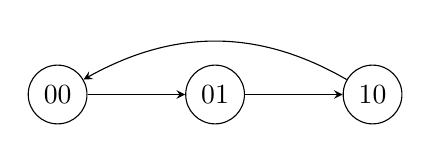
\begin{tikzpicture}[->, >=stealth]
  \node[draw,circle] (s0) at (0,0) {00};
  \node[draw,circle] (s1) at (2,0) {01};
  \node[draw,circle] (s2) at (4,0) {10};
  \draw (s0) -- (s1);
  \draw (s1) -- (s2);
  \draw (s2) edge[bend right] (s0);
\end{tikzpicture}
\end{center}

\section*{题目4：带使能的模8计数器}

\textbf{题目}：设计带使能信号en的模8计数器。en=1时计数，en=0时保持。

\textbf{VHDL}：
\begin{lstlisting}
 if rising_edge(clk) then
  if en = '1' then
    cnt <= cnt + 1;  -- 3位自然溢出=模8
  end if;
end if;
\end{lstlisting}

\section*{题目5：带同步加载的模10计数器}

\textbf{题目}：设计带同步加载（load）的模10计数器。load=1时cnt = data\_in；load=0时正常计数（0-9）。

\textbf{VHDL}：
\begin{lstlisting}
 if rising_edge(clk) then
  if load = '1' then
    cnt <= data_in;
  elsif cnt = "1001" then
    cnt <= "0000";
  else
    cnt <= cnt + 1;
  end if;
end if;
\end{lstlisting}

\section*{题目6：递增/递减双向计数器}

\textbf{题目}：设计模16双向计数器。up=1递增，up=0递减。

\textbf{VHDL}：
\begin{lstlisting}
 if rising_edge(clk) then
  if up = '1' then
    cnt <= cnt + 1;
  else
    cnt <= cnt - 1;
  end if;
end if;
\end{lstlisting}

\section*{题目7：模10 BCD计数器带7段显示}

\textbf{题目}：设计模10 BCD计数器 + BCD-7段译码器。输出驱动7段数码管显示0-9。

\section*{题目8：模60计数器（秒/分计数器）}

\textbf{题目}：设计模60计数器用于时钟应用。输出秒/分的十位和个位。

\textbf{分析}：见第三部分第八章BCD模60计数器。

\section*{题目9：模24 BCD计数器}

\textbf{题目}：设计模24 BCD计数器。0-23循环。

\textbf{分析}：十位模3（0-2），个位模10（0-9）。清零条件：23。

\section*{题目10：模100 BCD计数器}

\textbf{题目}：设计两位BCD模100计数器（00-99循环）。

\textbf{分析}：个位每满10向十位进位。十位满9+个位满9（即99）时清零。

\section*{题目11：给定计数器时序图，推断模值}

\textbf{题目}：观察计数器Q2Q1Q0的波形：000→001→010→011→100→000→...。求模值。

\textbf{解}：出现了5个不同状态（000-100），所以模值=5。

\section*{题目12：给定VHDL推断模值}

\textbf{题目}：
\begin{lstlisting}
 if cnt = "1010" then cnt <= "0000";
else cnt <= cnt + 1;
\end{lstlisting}
求模值N。

\textbf{解}：清零条件是cnt=10(1010)，所以N=10+1=11？不对！
清零条件=cnt=1010=10，此时cnt还未计数到11就被清零了。
模值=清零条件值+1=10+1=11？再确认：cnt从0计到10清零，所以N=11。

\textbf{关键公式}：模值 = 清零比较值 + 1

\section*{题目13：分析计数器最大工作频率}

\textbf{题目}：4位行波进位加法器的进位链延迟为每个FA=2ns，D触发器$t_{setup}=1$ns，$t_{cko}=1$ns。求计数器的最大工作频率。

\textbf{分析}：
关键路径延迟 = $t_{cko}$ + 进位链延迟(4×2=8ns) + $t_{setup}$ = 1+8+1 = 10ns
$f_{max} = 1/10\text{ns} = 100\text{MHz}$

\section*{题目14：多个计数器级联的分析}

\textbf{题目}：模8计数器 + 模5计数器级联。总模值是多少？

\textbf{解}：模8每8拍产生一次进位，模5每收到进位+1。
总模值 = 8×5 = 40。

\textbf{通用公式}：级联总模值 = $M_1 \times M_2 \times \dots \times M_k$

\section*{题目15：BCD计数器的非法状态恢复}

\textbf{题目}：模10 BCD计数器可能因干扰进入非法状态(1010-1111)。设计自恢复逻辑。

\textbf{解}：
\begin{lstlisting}
 if cnt >= "1010" then  -- 非法状态
  cnt <= "0000";
elsif cnt = "1001" then
  cnt <= "0000";
else
  cnt <= cnt + 1;
end if;
\end{lstlisting}

\section*{题目16-20：综合应用题}

\subsection*{题目16：数字钟核心}
设计时分秒计数器（模60秒+模60分+模24时）。

\subsection*{题目17：带暂停的计数器}
Pause=1时暂停计数，pause=0时恢复。

\subsection*{题目18：带预置位的倒计时计数器}
从预置值倒计时到0，到0后重新加载预置值。

\subsection*{题目19：两相正交计数器}
输出两个相位差90度的方波（格雷码计数器的一种应用）。

\subsection*{题目20：用计数器实现序列检测}
计数器状态作为地址，ROM存放序列，输出+检测逻辑。

\begin{examtip}[计数器类题目的统一解法]
\textbf{第一步：}确定模值N
\textbf{第二步：}$k = \lceil \log_2 N \rceil$，确定位宽
\textbf{第三步：}清零条件 = N-1 的二进制
\textbf{第四步：}写VHDL模板（if cnt=N-1 then cnt<=0 else cnt<=cnt+1）
\textbf{第五步：}如果有级联，低位进位接高位时钟使能

\textbf{关键公式}：
\begin{itemize}
  \item 模值 = 清零比较值 + 1
  \item 总模值（级联）= $M_1 \times M_2$
  \item $2^N$模值不需要显式清零
\end{itemize}
\end{examtip}

\chapter{分频器考试变式题}

\section*{题目1：2分频器（直接取Q0）}

\textbf{题目}：用最简单的方法实现2分频器。

\textbf{分析}：计数器最低位Q0天然2分频。只需一个D触发器每拍翻转。

\textbf{VHDL}：
\begin{lstlisting}
process(clk, rst_n)
begin
  if rst_n = '0' then q <= '0';
  elsif rising_edge(clk) then q <= not q; end if;
end process;
\end{lstlisting}
\textbf{输出频率}：$f_{out} = f_{clk} / 2$

\section*{题目2：4分频器（直接取Q1）}

\textbf{题目}：用计数器实现4分频器。

\textbf{分析}：2位计数器，Q1=4分频。直接取Q1作为输出。

\textbf{VHDL}：
\begin{lstlisting}
signal cnt : std_logic_vector(1 downto 0);
process(clk) begin
  if rising_edge(clk) then cnt <= cnt + 1; end if;
end process;
clk_div4 <= cnt(1);  -- Q1天然4分频
\end{lstlisting}

\section*{题目3：10分频器（占空比50\%）}

\textbf{题目}：设计10分频器，占空比50\%。

\textbf{分析}：
\begin{itemize}
  \item 模10计数器（0-9）
  \item cnt 0-4输出0，cnt 5-9输出1
  \item 每个周期5拍低+5拍高
\end{itemize}

\textbf{VHDL}：
\begin{lstlisting}
signal cnt : std_logic_vector(3 downto 0);
process(clk, rst_n)
begin
  if rst_n = '0' then cnt <= "0000";
  elsif rising_edge(clk) then
    if cnt = "1001" then cnt <= "0000";
    else cnt <= cnt + 1; end if;
  end if;
end process;
clk_div10 <= '0' when cnt < "0101" else '1';  -- 0-4低, 5-9高
\end{lstlisting}

\section*{题目4：3分频器（占空比非50\%）}

\textbf{题目}：设计3分频器。

\textbf{分析}：
\begin{itemize}
  \item 模3计数器（0→1→2→0）
  \item 简单方案：cnt=0,1输出0，cnt=2输出1（1/3占空比）
  \item 50\%占空比方案：需要上升沿+下降沿双计数器
\end{itemize}

\section*{题目5：5分频器}

\textbf{题目}：设计5分频器。

\textbf{分析}：模5计数器，占空比3/5或使用双沿方法实现50\%占空比。

\section*{题目6：100分频器}

\textbf{题目}：用50MHz时钟产生500kHz信号，设计分频器。

\textbf{分析}：$M = 50\text{MHz} / 500\text{kHz} = 100$。模100计数器。

\textbf{VHDL}：
\begin{lstlisting}
constant M : integer := 100;
signal cnt : integer range 0 to M-1;
process(clk, rst_n)
begin
  if rst_n = '0' then cnt <= 0;
  elsif rising_edge(clk) then
    if cnt = M-1 then cnt <= 0; else cnt <= cnt + 1; end if;
  end if;
end process;
clk_out <= '0' when cnt < M/2 else '1';
\end{lstlisting}

\section*{题目7：秒脉冲发生器}

\textbf{题目}：用100MHz时钟产生1Hz秒脉冲。

\textbf{分析}：$M = 100,000,000$。需要27位计数器（$2^{26} < 10^8 < 2^{27}$）。

\section*{题目8：多级分频器}

\textbf{题目}：用2分频+5分频级联实现10分频。

\textbf{分析}：$M_{total} = M_1 \times M_2 = 2 \times 5 = 10$。

\section*{题目9：可调分频比的计数器}

\textbf{题目}：设计分频比可动态设置的分频器（DIV从1到16可调）。

\textbf{VHDL}：
\begin{lstlisting}
signal cnt : std_logic_vector(3 downto 0);
process(clk) begin
  if rising_edge(clk) then
    if cnt = DIV - 1 then cnt <= "0000";
    else cnt <= cnt + 1; end if;
  end if;
end process;
\end{lstlisting}

\section*{题目10：占空比可调的分频器}

\textbf{题目}：设计10分频器，占空比可调（高电平持续周期数DUTY可配置）。

\textbf{VHDL}：
\begin{lstlisting}
clk_out <= '0' when cnt < DUTY else '1';
\end{lstlisting}

\section*{题目11：正交分频器（I/Q输出）}

\textbf{题目}：设计分频器同时输出I和Q两路信号，Q比I延迟90度。

\textbf{分析}：需要4分频才能产生90度相位差。I从cnt[1]取，Q从特定比较值取。

\section*{题目12：50\%占空比的奇数分频器}

\textbf{题目}：设计占空比50\%的5分频器。

\textbf{分析}：使用正沿2分频 + 负沿2分频组合的方法。

\section*{题目13：给定分频器输出波形，推断分频比}

\textbf{题目}：输出信号每8个输入时钟周期完成一个完整周期，求分频比。

\textbf{解}：$M = 8$（8分频）。

\section*{题目14：分析Qn分频输出频率}

\textbf{题目}：时钟100MHz，求4位计数器Q0、Q1、Q2、Q3的输出频率。

\textbf{解}：
\begin{itemize}
  \item Q0: $100/2=50$MHz
  \item Q1: $100/4=25$MHz
  \item Q2: $100/8=12.5$MHz
  \item Q3: $100/16=6.25$MHz
\end{itemize}

\section*{题目15：分频器级联频率计算}

\textbf{题目}：100MHz → 5分频 → 7分频，最终输出频率？

\textbf{解}：$f_{out} = 100\text{MHz} / (5 \times 7) = 100/35 \approx 2.857\text{MHz}$

\begin{examtip}[分频器类题目的统一解法]
\begin{enumerate}
  \item \textbf{计算分频比}：$M = f_{in} / f_{out}$
  \item \textbf{设计模M计数器}
  \item \textbf{偶数分频：}cnt < M/2输出0，否则输出1
  \item \textbf{奇数分频：}用双沿技术实现50\%占空比
  \item \textbf{$2^N$分频：}直接取Qn输出（最简单）
  \item \textbf{级联：}总M = 各级M的乘积
\end{enumerate}
\end{examtip}

\chapter{移位寄存器考试变式题}

\section*{题目1：串并转换（SIPO）}

\textbf{题目}：设计一个4位串入并出移位寄存器。串行输入数据，4个时钟周期后并行输出完整4位数据。

\textbf{VHDL}：
\begin{lstlisting}
signal reg : std_logic_vector(3 downto 0);
process(clk) begin
  if rising_edge(clk) then
    reg <= si & reg(3 downto 1);  -- 串行右移
  end if;
end process;
po <= reg;
\end{lstlisting}

\textbf{逐拍分析（输入1011）}：
\begin{center}
\begin{tabular}{|c|c|c|}
\hline
拍 & 输入 & [Q3 Q2 Q1 Q0] \\
\hline
1 & 1 & [1 0 0 0] \\
2 & 0 & [0 1 0 0] \\
3 & 1 & [1 0 1 0] \\
4 & 1 & [1 1 0 1] \\
\hline
\end{tabular}
\end{center}

4拍后po=1101（数据反转了，因为右移）。如想保持顺序，用左移。

\section*{题目2：并串转换（PISO）}

\textbf{题目}：设计4位并入串出移位寄存器。先load并行数据，然后移位输出。

\textbf{VHDL}：
\begin{lstlisting}
signal reg : std_logic_vector(3 downto 0);
process(clk) begin
  if rising_edge(clk) then
    if load = '1' then
      reg <= data_in;
    else
      reg <= '0' & reg(3 downto 1);  -- 右移，高位补0
    end if;
  end if;
end process;
so <= reg(0);
\end{lstlisting}

\section*{题目3：双向移位寄存器}

\textbf{题目}：设计4位双向移位寄存器。dir=1右移，dir=0左移。

\begin{lstlisting}
 if dir = '1' then
  reg <= si_right & reg(3 downto 1);
else
  reg <= reg(2 downto 0) & si_left;
end if;
\end{lstlisting}

\section*{题目4：带并行装载的通用移位寄存器（74LS194风格）}

\textbf{题目}：设计类似74LS194的4位通用移位寄存器。支持：保持、右移、左移、并行装载四种模式。

\textbf{VHDL}：
\begin{lstlisting}
case mode is
  when "00" => null;                    -- 保持
  when "01" => reg <= si_r & reg(3 downto 1);  -- 右移
  when "10" => reg <= reg(2 downto 0) & si_l;  -- 左移
  when "11" => reg <= data_in;          -- 装载
end case;
\end{lstlisting}

\section*{题目5：桶形移位器}

\textbf{题目}：设计8位桶形移位器，一次可移0-7位（移位量由3位输入控制）。

\textbf{分析}：桶形移位器是纯组合逻辑（不需要时钟），本质上是多路选择器网络。

\section*{题目6：移位寄存器的延迟线应用}

\textbf{题目}：用移位寄存器实现4拍延迟线（输入信号延迟4个时钟周期后输出）。

\textbf{解}：4位移位寄存器，so输出 = 4拍前的si输入。

\section*{题目7：序列检测用移位寄存器方案}

\textbf{题目}：用移位寄存器+比较器检测序列1011（替代状态机方案）。

\textbf{分析}：4位移位寄存器存储最近4位输入。当reg="1011"时输出1。

\begin{lstlisting}
reg <= data_in & reg(3 downto 1);
detected <= '1' when reg = "1011" else '0';
\end{lstlisting}

\section*{题目8：8位移位寄存器}

\textbf{题目}：设计8位串入并出移位寄存器。

\textbf{答案}：位宽从4扩展到8，其他逻辑完全相同。

\section*{题目9：循环移位寄存器}

\textbf{题目}：设计循环移位寄存器（最低位移入最高位，不丢失数据）。

\textbf{VHDL}：
\begin{lstlisting}
reg <= reg(0) & reg(7 downto 1);  -- 循环右移
\end{lstlisting}

\section*{题目10：算术移位寄存器}

\textbf{题目}：设计算术右移寄存器（保持符号位不变）。

\begin{lstlisting}
reg <= reg(7) & reg(7 downto 1);  -- 算术右移：符号位不变
\end{lstlisting}

\section*{题目11：逻辑移位vs算术移位}

\textbf{题目}：比较逻辑左移和算术左移的区别。

\textbf{分析}：左移时逻辑移位和算术移位等价（都补0）。右移时：逻辑右移补0，算术右移补符号位。

\section*{题目12：移位寄存器实现乘除法}

\textbf{题目}：用移位寄存器实现×2和÷2运算。

\textbf{分析}：
\begin{itemize}
  \item 左移1位 = ×2（reg <= reg(6 downto 0) \& '0'）
  \item 右移1位 = ÷2（reg <= '0' \& reg(7 downto 1)）
\end{itemize}

\section*{题目13：给定移位寄存器初值和输入序列，推断最终状态}

\textbf{题目}：4位右移寄存器初值0000，输入序列1011。4拍后寄存器内容？

\textbf{解（逐拍）}：
\begin{itemize}
  \item 初始：[0000]
  \item 拍1(si=1)：[1000]
  \item 拍2(si=0)：[0100]
  \item 拍3(si=1)：[1010]
  \item 拍4(si=1)：[1101]
\end{itemize}

4拍后：[1101]

\section*{题目14：移位寄存器Testbench设计}

\textbf{题目}：为8位移位寄存器设计完整的Testbench，验证串入并出功能。

\section*{题目15：移位寄存器构建伪随机序列（LFSR）}

\textbf{题目}：用4位移位寄存器+反馈构建最大长度LFSR。

\textbf{分析}：反馈多项式$X^4 + X^3 + 1$。反馈=Q3 XOR Q2。
产生序列长度=$2^4-1=15$（全0状态除外）。

\begin{examtip}[移位寄存器类题目的统一解法]
\begin{enumerate}
  \item \textbf{右移：}\texttt{reg <= si \& reg(N-1 downto 1)}
  \item \textbf{左移：}\texttt{reg <= reg(N-2 downto 0) \& si}
  \item \textbf{循环：}\texttt{reg <= reg(0) \& reg(N-1 downto 1)}
  \item \textbf{并行装载：}\texttt{if load='1' then reg <= data\_in;}
  \item \textbf{串出：}reg(0)（右移）或 reg(N-1)（左移）
  \item \textbf{并出：}整个reg
\end{enumerate}
\end{examtip}

\chapter{环形计数器考试变式题}

\section*{题目1：4位环形计数器}

\textbf{题目}：设计4位环形计数器。初始状态1000，经历4个状态循环：1000→0100→0010→0001→1000。

\textbf{VHDL}：
\begin{lstlisting}
signal reg : std_logic_vector(3 downto 0);
process(clk, rst_n)
begin
  if rst_n = '0' then reg <= "1000";
  elsif rising_edge(clk) then
    reg <= reg(0) & reg(3 downto 1);
  end if;
end process;
\end{lstlisting}

\textbf{逐拍验证}：
\begin{center}
\begin{tabular}{|c|c|}
\hline
拍 & [Q3 Q2 Q1 Q0] \\
\hline
0 & [1 0 0 0] \\
1 & [0 1 0 0] \\
2 & [0 0 1 0] \\
3 & [0 0 0 1] \\
4 & [1 0 0 0] ✓ 循环 \\
\hline
\end{tabular}
\end{center}

\section*{题目2：8位环形计数器}

\textbf{题目}：设计8位环形计数器。初始10000000。8个状态循环。

\textbf{VHDL}：
\begin{lstlisting}
signal reg : std_logic_vector(7 downto 0);
reg <= reg(0) & reg(7 downto 1);  -- 8位环形右移
\end{lstlisting}

\section*{题目3：4位约翰逊计数器（扭环形）}

\textbf{题目}：设计4位约翰逊计数器。初始0000。产生8个状态。

\textbf{VHDL}：
\begin{lstlisting}
reg <= (not reg(0)) & reg(3 downto 1);
-- 状态序列：0000→1000→1100→1110→1111→0111→0011→0001→0000
\end{lstlisting}

\textbf{状态分析}：
\begin{center}
\begin{tabular}{|c|c|}
\hline
拍 & [Q3 Q2 Q1 Q0] \\
\hline
0 & [0 0 0 0] \\
1 & [1 0 0 0] \\
2 & [1 1 0 0] \\
3 & [1 1 1 0] \\
4 & [1 1 1 1] \\
5 & [0 1 1 1] \\
6 & [0 0 1 1] \\
7 & [0 0 0 1] \\
8 & [0 0 0 0] ✓ \\
\hline
\end{tabular}
\end{center}

\textbf{关键规律}：约翰逊计数器（N个DFF）= 2N个状态。

\section*{题目4：带自启动的环形计数器}

\textbf{题目}：环形计数器可能因干扰进入非法状态（如两个1同时为1）。设计自启动逻辑。

\textbf{分析}：检测非法状态并自动恢复到合法状态。

\textbf{VHDL}：
\begin{lstlisting}
 if reg = "0000" or (reg(3)='1' and reg(2)='1') or ... then
  reg <= "1000";  -- 恢复到合法状态
else
  reg <= reg(0) & reg(3 downto 1);
end if;
\end{lstlisting}

\section*{题目5：环形计数器vs二进制计数器比较}

\textbf{题目}：比较8状态环形计数器和8状态二进制计数器。

\begin{center}
\begin{tabular}{|l|c|c|}
\hline
 & \textbf{环形计数器} & \textbf{二进制计数器} \\
\hline
DFF数量 & 8个 & 3个（$\lceil\log_2 8\rceil$）\\
状态编码 & One-hot & Binary \\
解码复杂度 & 0（直接读）& 需要译码器 \\
最大速度 & 1级DFF延迟 & 进位链延迟 \\
\hline
\end{tabular}
\end{center}

\section*{题目6：左移环形计数器}

\textbf{题目}：设计左移环形计数器（1从右向左移动）。

\textbf{VHDL}：
\begin{lstlisting}
reg <= reg(2 downto 0) & reg(3);  -- 左移循环
-- 序列：0001→0010→0100→1000→0001
\end{lstlisting}

\section*{题目7：自校正约翰逊计数器}

\textbf{题目}：设计自校正的4位约翰逊计数器，能自动从非法状态恢复到合法状态。

\section*{题目8：用环形计数器做序列发生器}

\textbf{题目}：用4位环形计数器的Q输出作为序列输出。产生什么序列？

\textbf{解}：
Q3输出序列：1, 0, 0, 0, 1, 0, 0, 0, ...（周期4）
各Q输出产生不同相位的同一序列。

\section*{题目9：环形计数器的状态数推导}

\textbf{题目}：N位移位寄存器可构成多少种不同状态的环形计数器？

\textbf{解}：One-hot编码，N个状态。每个状态只有一个1。

\section*{题目10：约翰逊计数器的状态数推导}

\textbf{题目}：N位移位寄存器可构成多少种不同状态的约翰逊计数器？

\textbf{解}：2N个状态。

\section*{题目11：给定波形推断计数器类型}

\textbf{题目}：4位寄存器输出波形为：1000→0100→0010→0001→1000...。判断类型和状态数。

\textbf{解}：4位环形计数器，4个状态。

\section*{题目12：给定初值和反馈逻辑推断状态序列}

\textbf{题目}：5位移位寄存器初值11000，反馈=Q0 XOR Q1。推断前8个状态。

\textbf{分析}：这是LFSR的行为，需要逐拍计算反馈值并移位。

\section*{题目13：环形计数器的one-hot特性优势}

\textbf{题目}：为什么One-hot编码的环形计数器适用于高速设计？

\textbf{分析}：
\begin{itemize}
  \item 状态解码不需要任何组合逻辑（直接看哪个DFF=1）
  \item 关键路径只有1级DFF延迟（没有加法器进位链）
  \item 适合超高速状态机
  \item 代价：状态数 = DFF数（资源效率低）
\end{itemize}

\section*{题目14：用环形计数器实现时序控制器}

\textbf{题目}：用5位环形计数器实现一个5步时序控制器，每步对应一个控制信号。

\textbf{解}：Q4-Q0分别作为步骤1-5的控制信号。每个时钟周期只有一个信号有效。

\section*{题目15：扭环形计数器做分频器}

\textbf{题目}：4位扭环形计数器（8状态）。各Q输出的频率是多少？

\textbf{解}：每个Q完成一个完整周期需要8拍。
$$f_Q = f_{clk} / 8$$

\begin{examtip}[环形计数器类题目的统一解法]
\begin{enumerate}
  \item \textbf{结构：}移位寄存器 + Q输出反馈到输入
  \item \textbf{普通环形：}反馈同相 → N状态（N个DFF）
  \item \textbf{扭环形（约翰逊）：}反馈反相 → 2N状态
  \item \textbf{核心VHDL：}\texttt{reg <= reg(0) \& reg(N-1 downto 1)}（环形右移）
  \item \textbf{自启动：}检测非法状态，强制恢复到100...0
  \item \textbf{优点：}超快（无进位链），输出直接可用（无需译码）
  \item \textbf{缺点：}状态数=DFF数（资源效率低）
\end{enumerate}
\end{examtip}

\chapter{序列检测器考试变式题}

\section*{题目1：检测1011（重叠检测）}

\textbf{题目}：设计Mealy型序列检测器，检测1011（重叠检测）。画出状态图，写VHDL。

\textbf{状态定义}：
\begin{itemize}
  \item S0：未匹配
  \item S1：已匹配"1"
  \item S10：已匹配"10"
  \item S101：已匹配"101"
\end{itemize}

\textbf{关键状态转移}：
\begin{itemize}
  \item S101 + 输入1 → 检测到（detected=1），去S1（最后1位作为新序列的第一个1——\textbf{重叠}）
\end{itemize}

\section*{题目2：检测1011（非重叠检测）}

\textbf{题目}：设计Moore型序列检测器，检测1011（非重叠）。检测到后重新开始。

\textbf{关键区别}：S101 + 输入1 → 检测到，去S0（重新开始——\textbf{非重叠}）。

\section*{题目3：检测1101（重叠）}

\textbf{题目}：设计序列检测器，检测1101（重叠）。画状态图。

\textbf{状态定义}：
\begin{itemize}
  \item S0→S1→S11→S110（已匹配"110"）
  \item S110 + 1 = 检测到，去S1（重叠：最后的"1"作为新序列的第一个"1"）
  \item 注意：S11 + 输入1 = 仍留在S11（"111"中后两个"11"匹配了"11"前缀）
\end{itemize}

\section*{题目4：检测0101（重叠）}

\textbf{题目}：设计序列检测器，检测0101。

\textbf{状态}：S0→S01→S010→S0101→检测

\section*{题目5：检测1111（4个连续1）}

\textbf{题目}：设计检测连续4个1的序列检测器。

\textbf{状态}：
\begin{itemize}
  \item S0→S1(1)→S11(2)→S111(3)→(第4个1→检测)
  \item 任何时候输入0，回到S0
  \item S111 + 1 → detected=1，去S111（重叠：最后3个1可以作为新序列的前3个1）
\end{itemize}

\section*{题目6：检测1001}

\textbf{题目}：设计检测1001的序列检测器。

\textbf{状态}：S0→S1→S10→S100→S1001(检测)

\textbf{关键}：S10+0→S100。S100+1→检测。S100+0→S0（"1000"不匹配任何前缀）。

\section*{题目7：检测序列长度可配置}

\textbf{题目}：设计可检测任意4位序列的可编程序列检测器（目标序列TARGET可配置）。

\textbf{VHDL}：
\begin{lstlisting}
signal reg : std_logic_vector(3 downto 0);
reg <= data_in & reg(3 downto 1);
detected <= '1' when reg = TARGET else '0';
\end{lstlisting}
（这是用移位寄存器方案实现的可编程检测器）

\section*{题目8：同时检测1011和1101}

\textbf{题目}：设计电路同时检测1011和1101。

\textbf{分析}：合并两个状态机（状态共享）。状态包括所有可能的前缀。

\section*{题目9：010检测器（3位序列）}

\textbf{题目}：设计检测010的序列检测器。画状态图，写VHDL。

\textbf{状态}：S0→S01(已匹配01)→S010(检测到)

\textbf{状态转移}：
\begin{itemize}
  \item S0 + 0 → S01（"0"已经匹配了01的第一个bit）
  \item S01 + 1 → S010（检测到！）
  \item S01 + 0 → S01（"00"——最后的0仍然是有效的第一个bit）
  \item S010 + 0 → S01（检测后，最后的0作为新序列的第一个bit——重叠）
\end{itemize}

\section*{题目10：连续N个相同bit检测器}

\textbf{题目}：设计检测连续N个0（或连续N个1）的检测器。

\textbf{分析}：用一个计数器统计连续相同bit的个数。

\section*{题目11：Moore vs Mealy检测器比较}

\textbf{题目}：比较Moore型和Mealy型序列检测器检测1011的差异。

\begin{center}
\begin{tabular}{|l|c|c|}
\hline
 & \textbf{Moore型} & \textbf{Mealy型} \\
\hline
输出决定因素 & 仅当前状态 & 当前状态+输入 \\
检测延迟 & 需进入检测状态（晚1拍）& 同一拍输出 \\
状态数 & 多1个（需要"检测到"状态）& 少1个 \\
输出稳定性 & 整个周期稳定 & 输入变化时可能变 \\
\hline
\end{tabular}
\end{center}

\section*{题目12：序列检测器+计数器统计检测次数}

\textbf{题目}：扩展1011检测器，增加计数功能：统计检测到多少次1011。

\textbf{VHDL}：
\begin{lstlisting}
signal detect_count : integer range 0 to 255;
process(clk) begin
  if rising_edge(clk) then
    if detected = '1' then
      detect_count <= detect_count + 1;
    end if;
  end if;
end process;
\end{lstlisting}

\section*{题目13：带超时检测的序列检测器}

\textbf{题目}：如果连续输入超过16个时钟周期未检测到序列，输出timeout信号。

\textbf{分析}：增加一个超时计数器。每次状态变化时清零，超过阈值时timeout=1。

\section*{题目14：双向序列检测器}

\textbf{题目}：检测1011和1101中任意一个（两者共享前缀"1"）。

\textbf{状态图合并}：
S0 → S1(1) → 分支：S10(10) 或 S11(11)
S10 → S101(101) →(1→检测1011)
S11 → S110(110) →(1→检测1101)

\section*{题目15：格雷码序列检测}

\textbf{题目}：输入是并行3位格雷码，检测格雷码序列"000→001→011→010→110"的出现。

\textbf{分析}：这是并行输入的序列检测。状态机根据并行输入值转移。

\section*{题目16：含"无关项"的序列检测}

\textbf{题目}：检测1x1x（第一位和第三位为1，其他任意）。例：1010匹配，1111也匹配。

\textbf{分析}：用移位寄存器存储最近4位，只比较第3位和第1位是否为1。

\section*{题目17：给定状态图，写VHDL}

\textbf{题目}：给定状态转移图，写出对应的VHDL状态机代码。

\textbf{秒杀方法}：
\begin{enumerate}
  \item type定义状态枚举（每个状态一个枚举值）
  \item process敏感列表=clk, rst_n
  \item case语句逐个处理每个状态的转移
  \item 输出逻辑根据状态（Moore）或状态+输入（Mealy）赋值
\end{enumerate}

\section*{题目18：给定输入序列和状态机，求输出}

\textbf{题目}：1011检测器（重叠），输入=1011011。问输出序列。

\textbf{解（逐拍分析）}：
\begin{center}
\begin{tabular}{|c|c|c|c|c|c|c|c|}
\hline
拍 & 1 & 2 & 3 & 4 & 5 & 6 & 7 \\
\hline
输入 & 1 & 0 & 1 & 1 & 0 & 1 & 1 \\
状态 & S1 & S10 & S101 & S1 & S10 & S101 & S1 \\
输出 & 0 & 0 & 0 & \textbf{1} & 0 & 0 & \textbf{1} \\
\hline
\end{tabular}
\end{center}

输出序列：0 0 0 1 0 0 1（第4拍和第7拍检测到）

\section*{题目19：状态编码优化}

\textbf{题目}：1011检测器有4个状态。分别用二进制编码和One-hot编码实现。比较资源消耗。

\textbf{分析}：
\begin{itemize}
  \item 二进制编码：2个DFF（$2^2=4$状态），需要组合逻辑解码
  \item One-hot编码：4个DFF，无需解码逻辑
  \item 速度vs面积的经典权衡
\end{itemize}

\section*{题目20：复杂序列检测——检测101后跟11}

\textbf{题目}：检测序列"101"后紧跟"11"（即检测10111）。

\textbf{状态}：S0→S1→S10→S101→S1011→S10111(检测)

\begin{examtip}[序列检测器类题目的统一解法——核心步骤]
\textbf{第一步：理解目标序列。}确定要检测的序列是什么。

\textbf{第二步：确定状态。}每个状态 = 已匹配的序列前缀。
\begin{itemize}
  \item S0 = 匹配0位
  \item S前缀名 = 匹配了前缀名的全部内容
  \item 最后一个前缀 = 差1位就匹配完整序列
\end{itemize}

\textbf{第三步：画状态转移图。}对每个状态，考虑输入0和1分别去哪。

\textbf{第四步：写状态转移表。}整理为表格形式。

\textbf{第五步：写VHDL。}
\end{examtip}

\begin{lstlisting}
type state_type is (...);
signal state : state_type;
process(clk, rst_n) begin
  if rst_n='0' then state <= S0;
  elsif rising_edge(clk) then
    case state is
      when S0 => if din='1' then state <= S1; end if;
      when S1 => if din='0' then state <= S10; end if;
      ...
    end case;
  end if;
end process;
\end{lstlisting}

\begin{examtip}[序列检测器类题目的统一解法——核心步骤（续）]

\textbf{第六步：区分重叠/非重叠。}
\begin{itemize}
  \item \textbf{重叠检测：}检测到后，分析当前输入的后几位能否作为下一次匹配的前缀
  \item \textbf{非重叠检测：}检测到后直接回S0
\end{itemize}

\textbf{常考序列状态数速查：}
\begin{itemize}
  \item 检测1011：4个状态（S0, S1, S10, S101）
  \item 检测1101：4个状态（S0, S1, S11, S110）
  \item 检测0101：4个状态（S0, S01, S010, S0101）
  \item 检测1111：4个状态（S0, S1, S11, S111）
  \item 检测010：3个状态（S0, S01, S010）
  \item 检测101：3个状态（S0, S1, S10）
\end{itemize}
\end{examtip}

\section{全书总结}

恭喜你读到这里。

现在回顾一下，你掌握了：

\begin{enumerate}
  \item \textbf{7个组合逻辑电路}：编码器、译码器、BCD译码器、MUX、比较器、加法器、级联MUX
  \item \textbf{D触发器的底层模型}：1 bit存储，时钟沿驱动，$Q(n+1)=D(n)$
  \item \textbf{计数器的统一框架}：所有模值计数器 = 同一个模板改N-1
  \item \textbf{分频器的本质}：计数器的一个应用，Qn天然分频
  \item \textbf{序列发生器的多种方案}：计数器+映射、状态机、移位寄存器
  \item \textbf{移位寄存器的数据流动}：逐拍分析，数据如水流过管道
  \item \textbf{环形计数器的循环}：反馈形成闭环，1在环中无限循环
  \item \textbf{序列检测器的状态机}：状态=已匹配前缀，输入决定下一状态
  \item \textbf{VHDL与硬件的对应}：每行代码对应什么硬件
  \item \textbf{100+道变式题的解题能力}
\end{enumerate}

\textbf{核心信念}：

\begin{center}
\fbox{%
\begin{minipage}{0.85\textwidth}
\large

不是背代码。

是理解电路。

理解它为什么存在。

理解它怎么工作。

理解状态如何在时钟推动下变化。

要相信，世间万般变体设计，皆是本源规则注定的衍生结果！
\end{minipage}%
}
\end{center}

祝好。
\end{chapter}


\end{document}
